% !TeX program = xelatex
% !TeX encoding = UTF-8
\documentclass{MathModeling}
\usepackage{mwe,color,float}
\usepackage[linesnumbered,ruled]{algorithm2e}
\usepackage{setspace}
\usepackage{colortbl}
\usepackage{tablefootnote}
\everymath{\displaystyle}

\extrafloats{500}
\timu{\textbf{Wordle游戏探讨及预测}}
\keyword{自然语言分析;XGBoost;随机森林;K-means单词聚类;SVM-OVR}
\begin{document}
\setcounter{page}{1}
\pagestyle{fancy}
	\begin{abstract}
		Wordle是一款具有简单绘画风格的猜词小游戏,在网络上非常流行,Wordle玩家会在各种社交平台上分享他们的战绩。优化游戏设计、提高用户体验,对提高受欢迎程度、娱乐价值至关重要。因此,本文采用了回归、聚类、预测、自然语言处理等方法,对Wordle游戏的数据进行分析。

		{\heiti 针对问题一},\textbf{需要分析Wordle的Twitter玩家每日报告结果变化情况,并建立模型来解释这种变化;对2023年5月15日的报告结果进行预测,并给出置信水平;分析单词属性是否会影响困难模式下玩家尝试次数的比例,并解释原因。}由于数据集仅有2022年的一部分,且问题需要预测2023年5月15日,因此,本文首先对2023年相关数据进行\textbf{爬取}。之后对数据进行合并整理,同时对\textbf{百分比异常值、异常单词、人数异常值}进行\textbf{预处理}。在此基础上,本文对游戏\textbf{生命周期}进行分析,建立\textbf{XGBoost回归预测模型},分别对每日报告玩家总数及选择困难模式游戏玩家人数进行数据学习、测试、预测。两模型\textbf{拟合优度}$\boldsymbol{R^2}$分别可达$\boldsymbol{0.9957}$及$\boldsymbol{0.9959}$,其\textbf{MAE}、\textbf{MSE}、\textbf{RMSE}均较小,具体见\textcolor{blue}{\cref{tab:XGBoost预测结果}}。最终得到2023年5月15日报告总人数区间结果为$\boldsymbol{\left[17831,18352\right]}$,选择困难模式游戏人数为$\boldsymbol{\left[1856,1892\right]}$,且结果建立在$\boldsymbol{95\,\%}$的\textbf{置信水平}上。此外本文还对单词进行属性分析,构造出\textbf{单词词性、元音字母个数、每位字母在英文中出现频率、单词中重复字母个数}等特征,绘制\textbf{皮尔逊相关系数热力图},分析单词属性与玩家游戏中的表现的关联性,具体结果见{\heiti \textcolor{blue}{\nameref{单词属性与玩家游戏中的表现关联分析}}}。

		{\heiti 针对问题二},\textbf{需要对给定的单词预测当天玩家游戏尝试次数百分比分布情况,并分析模型的不确定性因素。}因此,本文综合\textbf{XGboost,线性预测,随机森林,LightGBM回归模型}进行分析,依据\textbf{MAE}、\textbf{MSE}、\textbf{RMSE}、$\boldsymbol{R^2}$,选择最优的算法进行预测,模型效果比较见\textcolor{blue}{\cref{tab:回归模型指标}}。最终本文选择随机森林模型对单词“EERIE”进行预测,其百分比结果为$\boldsymbol{\left[0.17,4.73,16.24,30.72,27.86,14.03,6.08\right]}$,模型\textbf{MAE}控制在$\boldsymbol{2\,\%}$内,效果良好。此外,本文还对模型的不确定性因素进行分析,具体结果见{\heiti \textcolor{blue}{\nameref{不确定性因素分析}}}。

		{\heiti 针对问题三},\textbf{需要根据单词难度对单词分类,预测单词“EERIE”难度,同时给出模型的预测精度。}因此本文结合问题一所构造的特征及相关指标,建立\textbf{K-means单词聚类}模型,通过\textbf{肘部法则}确定最优$\boldsymbol{k=5}$,在此基础上将单词划分为\textbf{“非常容易”“容易”“中等”“困难”“非常困难”5个类别}。再利用\textbf{SVM-OVR多分类}模型,在已划分难度的数据集上学习,对单词“EERIE”难度进行预测,最终其被归类为\textbf{“困难”},模型精度可达$\boldsymbol{94.74\,\%}$。此外本文针对该模型进行\textbf{灵敏度分析检验},绘制其\textbf{混淆矩阵热力图、分类报告、ROC/AUC曲线}等,最终确定模型效果优良,具体见{\heiti \textcolor{blue}{\nameref{灵敏度分析}}}。

		{\heiti 针对问题四},本文结合\textbf{散点、核密度、折线、雷达、小提琴等图}进行分析,得出更深层次结论,具体分析结果见{\heiti \textcolor{blue}{\nameref{问题四}}}。

		{\heiti 针对问题五},本文综合上述问题的分析,向纽约时报的谜题编辑总结结果并提出相关建议,本文提供英文及中文信函各一份,具体见{\heiti \textcolor{blue}{\nameref{问题五}}}。

		最后,本文对所建立的模型进行中肯评价、提出改进措施,并对模型进行一定推广。
	\end{abstract}

	\section{问题的提出}
	\subsection{问题背景}
	作为一款单词猜谜游戏,Wordle每天都为玩家提供一个真正的英语单词作为谜题,现已推出60多种语言版本,本文以英文版本为例。其玩法为:玩家在6次或更少次数内猜出一个5个字母的单词以解决谜题。在此过程中,玩家每一次进行的猜测必须为真实存在的单词,提交后系统将对单词进行检测,若该位置显示为绿色则代表谜底单词含有该字母,且其位置正确;若为黄色则代表该字母存在但所在位置错误;若为灰色则谜底中不包含此字母。玩家可选择“常规模式”及“困难模式”进行挑战,其中在“困难模式”下玩家若找到谜底中包含的字母,即显示绿色及黄色砖块,在其后的猜测的单词中必须包含这些字母。游戏两种模式玩法见\textcolor{blue}{\cref{fig:简单模式游戏}}及\textcolor{blue}{\cref{fig:困难模式游戏}}。Wordle官方统计了在Twitter上分享的每一天玩家通关所需次数,需要对该数据进行分析并预测未来的结果。
	\begin{figure}[H]
		\centering
		\begin{minipage}{0.48\linewidth}
			\centering
			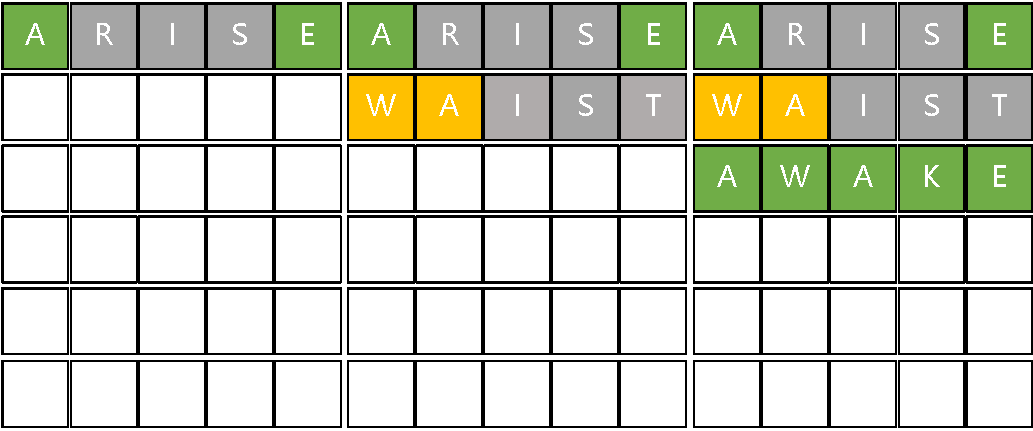
\includegraphics[width=0.96\linewidth]{简单模式图.pdf}
			\caption{常规模式}
			\label{fig:简单模式游戏}
		\end{minipage}
		%\qquad
		\begin{minipage}{0.48\linewidth}
			\centering
			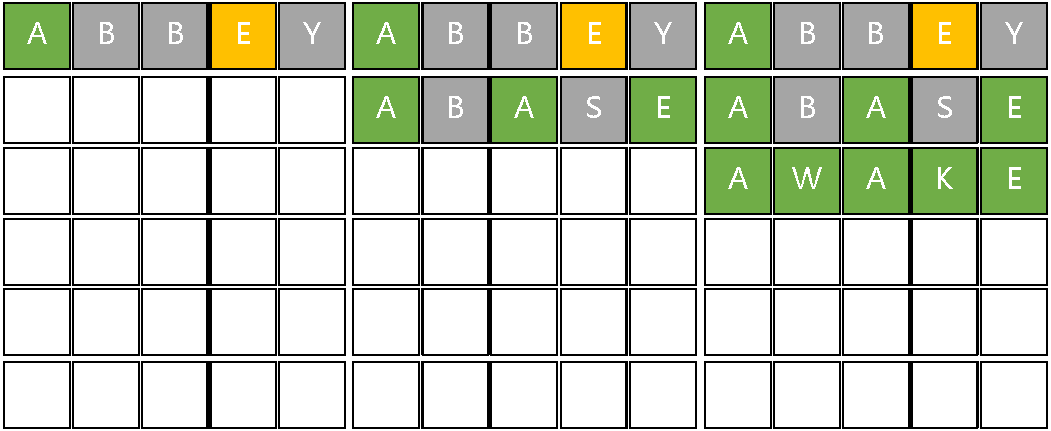
\includegraphics[width=0.96\linewidth]{困难模式图.pdf}
			\caption{困难模式}
			\label{fig:困难模式游戏}
		\end{minipage}
	\end{figure}

	\subsection{问题要求}
	\begin{itemize}
		\item \textbf{问题一}:官方所提供报告的结果每天数量均存在差异,建立一个模型以解释该差别;同时需要预测2023年5月15日报告结果的数量区间;此外还分析单词属性对于困难模式得分比例是否存在影响,并解释原因。
		\item \textbf{问题二}:建立模型预测未来谜底单词的报告结果相关百分比,说明模型预测的不确定性因素,并对单词“EERIE”进行预测。
		\item \textbf{问题三}:建立一个依据单词难度分类的模型对谜底单词分类。确定各类别中谜底单词属性,并对单词“EERIE”的难度进行分析,并分析模型的精度。
		\item \textbf{问题四}:进一步分析数据集中其他有趣的特征。
		\item \textbf{问题五}:写一封信函向《纽约时报》的谜底编辑总结分析结果。
	\end{itemize}

	\section{问题的分析}
	\subsection{问题的整体分析}
	该题是一个以热门游戏Wordle为背景的数据分析,自然语言处理,预测类问题。

	\textbf{从分析目的看},本题需要以单词的属性进行分析,筛选出影响玩家得分比例的主要因素,确定各分类相关联的给定单词的属性并总结,量化结果。同时还须对玩家的得分结果进行预测与研究,为《纽约时报》的谜题编辑提供参考,以进一步优化Wordle游戏。因此本题主要需要完成以下几方面的任务:{\heiti 其一},分析每日报告结果数量的变化情况;{\heiti 其二},确定单词属性与困难模式游玩得分的关系;{\heiti 其三},预测特定单词玩家尝试次数的百分比;{\heiti 其四},分析单词属性与单词难度的关联性;{\heiti 其五},进一步探讨数据集具有的有趣特征;{\heiti 其五}:写一封信函向《纽约时报》的谜底编辑总结分析结果。

	\textbf{从数据来源、特征看},本题的数据来源于2022年2月7日至2022年12月31日Twitter玩家分享游戏结果,数据包括“日期”“编号”“谜底单词”“答案提交数”“困难模式参与数”“1$\sim$7次尝试分布比例”。但未提高对数据的分析能力,提升预测效果,挖掘更多有效信息,我们将对2023年数据进行爬取,构造与附件数据一致的数据,两者综合进行分析。同时我们发现数据具有高维,量纲不一致等特点,且数据体量较大,因此,本题相对复杂,需对数据进行一定的预处理,以便于后续分析。

	\textbf{从模型的选择看},本题数据的时间跨度大,维度较高,且需预测未来的报告数和相关百分比的分布、基于单词难度对单词进行分类。因此本文选择XGboost回归模型、随机森林回归模型进行预测分析,同时利用K-means模型对单词进行分类,在该分类基础上建立数据标签,并采用SVM模型对单词“EERIE”进行预测。

	\textbf{从编程软件的选择看},本题为数据分析类,需要进行数据预处理、数据分析、数据可视化,并依据各设问建立不同类别的模型,因此我们选择Python Jupyter Notebook对问题进行求解,其交互式的编程范式及轻量化,方便且高效。
	
	\subsection{问题一的分析}
	问题一的核心目的有以下几点:{\heiti 其一},\textbf{对报告数据进行预处理,去伪存真};{\heiti 其二},\textbf{研究每日结果数据的变化};{\heiti 其三},\textbf{预测2023年5月15日报告结果数量,并建立一个合理区间};{\heiti 其四},\textbf{研究分析单词属性与困难模式得分的关系}。对于给定的数据集,我们发现部分数据在正确性,完整度性等方面存在一定缺陷,因此我们须对数据集进行预处理。由于附数据体量较大,因此我们将将总人数,选择困难模式人数及其变化率数据可视化,直观分析变化规律并建立普适性预测模型。同时我们还考虑到游戏人数数据等不符合正态分布,因此我们放弃线性回归而选择XGBoost模型进行回归预测。此外我们对单词进行属性分析,利用Python自然语言处理nltk库,建立单词的属性模型,并绘制皮尔逊相关系数热力图分析其中的关系。

	\subsection{问题二的分析}
	问题二的核心目的在于\textbf{预测报告结果中玩家尝试次数分布的情况,并分析模型的不确定性因素}。因此我们根据问题一中已构造的单词属性,综合XGboost,线性分析,随机森林,LightGBM等回归模型的MSE、RMSE、MAE、$R^2$指标,对模型进行分析,选择最优模型,建立预测给定日期的单词玩家尝试次数分布的百分比的普适性模型,对2023年5月15日单词“EERIE”进行预测,最后分析模型中的不确定性因素。

	\subsection{问题三的分析}
	问题三的核心目的在于\textbf{根据单词难度对单词进行分类,预测单词“EERIE”所属难度,同时给出模型的预测精度}。因此我们结合问题一所构造的特征及相关指标,对样本数据进行K-means聚类分析,并结合肘部法则选择合适的$k$值,绘制PCA降维聚类结果散点图,并计算聚类轮廓系数,分析聚类效果。在对样本数据进行分类后,将难度定义为词汇的分类标准,采用SVM多分类预测模型对分类的结果进行更详细的定性及定量分析。最后对单词“EERIE”进行分析预测,确定其难度。此外我们还需对模型进行合理性分析,讨论分类模型的准确性。

	\subsection{问题四的分析}
	对于该问题,我们需要更深次地挖掘数据,发现更多有趣的信息及结论,因此在这里我们将从多方面进行分析,同时绘制可视化图形如散点图、核密度图、日变化图、雷达图、小提琴图等,便于对数据内在特征进行分析。

	\subsection{问题五的分析}
	对于该问题,我们需要总结问题一至四分析结果,并向纽约时报的谜题编辑总结本
	文结果并提出相关建议。本文将提供英文及中文信函各一份,方便读者阅读。
	
	\section{模型的假设}
	\begin{itemize}
		\item \textbf{假设一}:假设个体在单词认知能力上差异较小。
		\item \textbf{假设二}:假设《纽约时报》每一天的谜底单词均随机抽取,不受人为等因素干扰。
		\item \textbf{假设三}:假设每日参与游戏人数不会出现较为明显的波动,在一定范围内稳定。
		\item \textbf{假设四}:假设若玩家在六次及以内未能成功猜出谜底单词,则游戏失败。并将游戏失败的玩家视作进行7次尝试。
	\end{itemize}
	\section{符号说明}
	\begin{center}
		\begin{tabularx}{0.7\textwidth}{c@{\hspace{1pc}}|@{\hspace{2pc}}X}
			\Xhline{0.08em}
			符号 & \multicolumn{1}{c}{符号说明}\\
			\Xhline{0.05em}
			$\mu$ & 样本平均数 \\
			$\sigma$ & 样本标准差 \\
			$y$ & 因变量实际值\\
			$\hat{y}$ & 因变量预测值\\
			$L^{\left(t\right)}$ & 目标函数\\
			$\rho\left(x,y\right)$ & 皮尔逊相关系数 \\
			\Xhline{0.08em}
		\end{tabularx}
	\end{center}

	\textbf{注:}这里并未列出其余变量,这是由于它们在不同小节处有不同的含义,同时该表中也未列出专有定义的变量,这些变量在使用时会在相应位置进行详细说明。
	\section{模型的建立与求解}
	本文模型的建立与求解部分主要分为数据的准备,模型的建立、求解、结果分析。\textcolor{blue}{\footnote{本文所有可视化图示均为矢量图,若读者在阅读时发现图示字体过小,可适当放大PDF页面,详细查看图示数据等。此外,本文所有图示、表格均已交叉引用,读者阅读PDF时可点击对应图表,进行跳转。}}
	\begin{itemize}
		\item \textbf{数据的准备}:首先爬取2023年相关数据,提高模型分析的准确性。再者,对于构建的新数据集进行预处理,方便后续模型的建立,减少异常值对分析的影响;
		\item \textbf{模型的建立、求解、结果分析}:对于整理完成的新数据集,本文依据其特点,建立合适的回归、聚类、分类预测模型,并进行多种数据可视化,分析模型效果。
	\end{itemize}

	\subsection{数据的准备}
	本部分我们需要爬取2023年的数据,以提高模型分析数据的准确性。同时还需要对数据集进行一定的预处理,对错误值进行修正,以便后续模型的建立。本部分我们所利用的数据收集网站见\textcolor{blue}{\cref{tab:数据来源}}。

\begin{table}[H]
	\centering
	\caption{数据来源}
	\scalebox{0.85}{
	  \begin{tabular}{cc}
	  \toprule
	  \textbf{网址} & \textbf{描述} \\
	  \midrule
	  \url{https://m.stockq.org/life/wordle-history.php\#all} & Wordle每日答案统计 \\
	  \url{https://twitter.com/WordleStats} & Wordle每日报告结果 \\
	  \bottomrule
	  \end{tabular}}
	\label{tab:数据来源}
\end{table}
	\subsubsection{2023年数据爬取}
	原数据集统计的为2022年2月7日至2022年12月31日的情况,缺少2023年数据,而问题需要预测2023年5月15日数据,因此为提高模型精度,我们爬取2023年相关数据,并与原数据集进行合并,使得在游戏编号、时间方面连续。新数据集读者可在附件中查阅。其中部分数据见\textcolor{blue}{\cref{tab:2023年部分数据}},新数据集收集截止至2023年4月25日。
\begin{table}[H]
	\centering
	\caption{2023年部分数据}
	\scalebox{0.80}{
	  \begin{tabular}{ccccc}
	  \toprule
	  \textbf{Date}  & \textbf{Contest number} & \textbf{Word}  & \textbf{Number of reported results} & \textbf{Number in hard mode} \\
	  \midrule
	  2023/1/1 & 561   & whine & 22072 & 2132 \\
	  2023/1/2 & 562   & skirt & 22252 & 2094 \\
	  2023/1/3 & 563   & antic & 22018 & 2072 \\
	  2023/1/4 & 564   & layer & 22394 & 2207 \\
	  2023/1/5 & 565   & sleek & 22283 & 2078 \\
	  \bottomrule
	  \end{tabular}}
	\label{tab:2023年部分数据}
\end{table}

	\subsubsection{百分比异常值}
	根据对原数据集中尝试次数百分比的理解,其7次累计和应为$1$,因此我们计算数据中玩家尝试次数百分比的累计和,我们发现,除游戏编号为$281$的数据累计百分比为$126\,\%$,其余数据均在$\left(100\pm2\right)\,\%$的范围内,因此我们有理由认为该天存在统计误差,并记为异常值。

	\subsubsection{异常单词的修正}
	根据Wordle游戏规则,每日谜底单词均为5个字母长度,因此我们对原数据集所有单词进行分析,筛选出字母数不为5个的单词,并依据Wordle游戏每日单词统计的数据与游戏编号进行比对,将上述错误单词替换为正确单词,更换结果见\textcolor{blue}{\cref{tab:单词修正}}。
\begin{table}[H]
	\centering
	\caption{单词修正}
	\scalebox{0.85}{
	  \begin{tabular}{cccc}
	  \toprule
	  \textbf{游戏编号} & \textbf{时间} & \textbf{异常单词} & \textbf{替换单词} \\
	  \midrule
	  207   & 2022/1/12 & favor \textcolor{blue}{\tablefootnote{该单词错误原因是在表格数据中其后有一空格,该空格会影响后续问题的解决。}} & favor \\
	  314   & 2022/4/29 & tash  & trash \\
	  525   & 2022/11/26 & clen  & clean \\
	  545   & 2022/12/16 & rprobe & probe \\
	  \bottomrule
	  \end{tabular}}
	\label{tab:单词修正}
\end{table}
  
	\subsubsection{人数异常值}
	为了更好地初步发现异常值,我们绘制出每日游戏报告结果总人数及选择困难游戏模式人数变化图,如\textcolor{blue}{\cref{fig:总人数及选择困难游戏模式人数变化图}}。观察该图,我们可以发现,2022年11月30日总人数突然减少明显,但其对应的选择困难人数并未有明显变化,且两者数据相近。因此,这里我们定义其为离群点,其明显不符合发展变化规律,对其的处理,我们将再下文展开分析。

	\begin{figure}[H]
		\centering
		\begin{minipage}{0.48\linewidth}
			\centering
			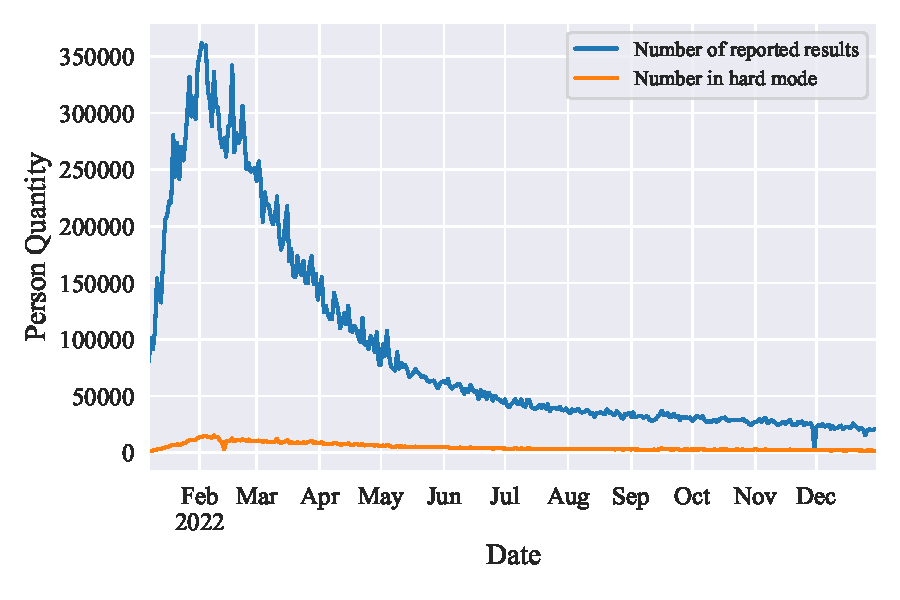
\includegraphics[width=0.96\linewidth]{报告结果每日变化.pdf}
			\caption{总人数及选择困难游戏模式人数日变化}
			\label{fig:总人数及选择困难游戏模式人数变化图}
		\end{minipage}
		%\qquad
		\begin{minipage}{0.48\linewidth}
			\centering
			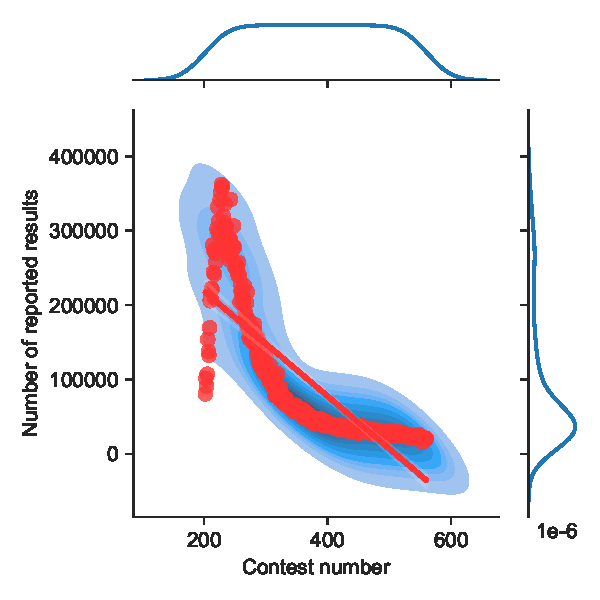
\includegraphics[width=0.62\linewidth]{核密度估计值.pdf}
			\caption{每日报告结果变化趋势}
			\label{fig:每日报告结果变化趋势}
		\end{minipage}
	\end{figure}
	% \begin{figure}[H]
	% 	\centering
	% 	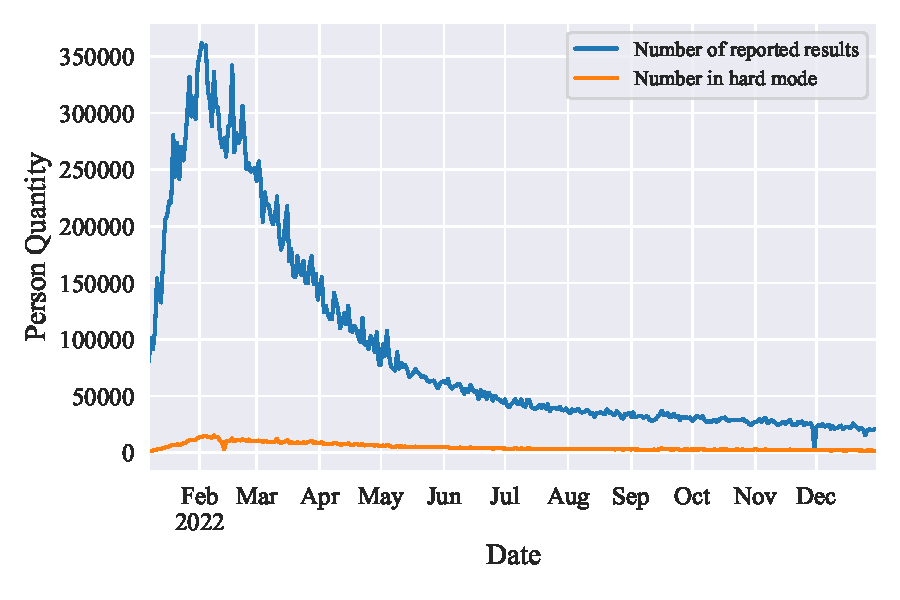
\includegraphics[width=0.55\textwidth]{报告结果每日变化.pdf}
	% 	\caption{总人数及选择困难游戏模式人数日变化}
	% 	\label{fig:总人数及选择困难游戏模式人数变化图}
	% \end{figure}
	% \begin{figure}[H]
	% 	\centering
	% 	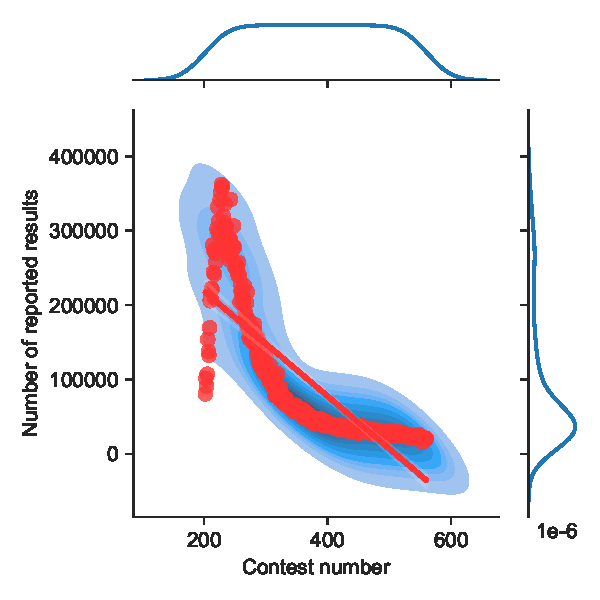
\includegraphics[width=0.5\textwidth]{核密度估计值.pdf}
	% 	\caption{每日报告结果变化趋势}
	% 	\label{fig:每日报告结果变化趋势}
	% \end{figure}

	同时我们还计算出每日选择困难人数占总人数的比例,绘制出每日选择困难模式人数频率变化及变化率图示,见\textcolor{blue}{\cref{fig:每日选择困难模式人数频率变化}}及\textcolor{blue}{\cref{fig:每日选择困难模式人数频率变化率}}。

	\begin{figure}[H]
		\centering
		\begin{minipage}{0.48\linewidth}
			\centering
			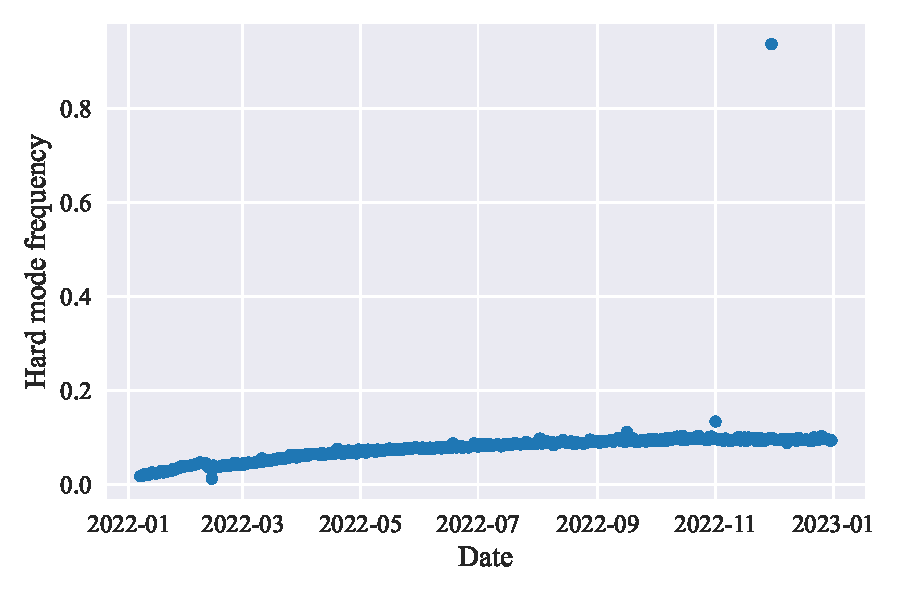
\includegraphics[width=0.76\linewidth]{每日选择困难模式人数频率变化.pdf}
			\caption{每日选择困难模式人数频率变化}
			\label{fig:每日选择困难模式人数频率变化}
		\end{minipage}
		%\qquad
		\begin{minipage}{0.48\linewidth}
			\centering
			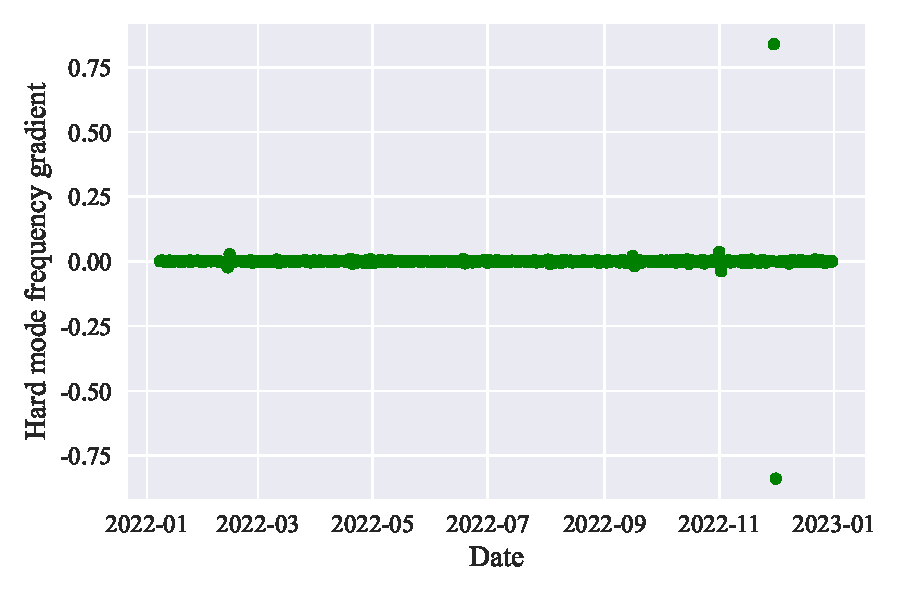
\includegraphics[width=0.76\linewidth]{每日选择困难模式人数频率变化率.pdf}
			\caption{每日选择困难模式人数频率变化率}
			\label{fig:每日选择困难模式人数频率变化率}
		\end{minipage}
	\end{figure}
	通过观察上述两幅图,我们可以清晰发现异常值,但也存在部分图示上难以鉴别的离群点,因此这里我们设定变化率阈值为$0.02$,若每日变化率绝对值超过该阈值,且在相邻两天内变化率绝对值超过该阈值,则定义其为离群点,对其进行处理。这是由与若某一天突变严重,会引起当天与后一天变化率均会超过阈值,而真正地异常值应为首次超过的那一天。但异常值为总人数还是选择困难游戏人数,我们还需要结合改日前后几天数据记性判断。通过筛选,我们得到异常数据,见\textcolor{blue}{\cref{tab:异常数据}}。
\begin{table}[H]
	\centering
	\caption{异常数据分析}
	\scalebox{0.85}{
	  \begin{tabular}{cccccc}
	  \toprule
	  \textbf{游戏编号} & \textbf{当日单词} & \textbf{游戏总人数} & \textbf{选择困难模式人数} & \textbf{选择困难人数变化率} & \textbf{异常值} \\
	  \midrule
	  239   & robin & 277471 & 3249  & -0.022787  & 3249 \\
	  240   & ultra & 261521 & 10343 & 0.027840  & / \\
	  500   & piney & 27502 & 3667  & 0.036272  & 3667 \\
	  501   & inept & 27670 & 2640  & -0.037926  & / \\
	  529   & study & 2569  & 2405  & 0.838601  & 2569 \\
	  530   & eject & 22628 & 2200  & -0.838937  & / \\
	  \bottomrule
	  \end{tabular}}
	\label{tab:异常数据}
\end{table}

	\subsubsection{异常值处理}
对于异常值的处理,为了尽可能保留数据信息,我们采用拉格朗日插值法,对上述异常数据进行修正。\textbf{拉格朗日插值法(Lagrange's Interpolation)}是一种多项式插值的方法。对于给定的$n+1$个坐标不同的点,其可以给出一个恰好经过这$n+1$个点的多项式函数。拉格朗日基本多项式(插值基函数)如下
\begin{equation}
	l_{j}\left(x\right)=\prod_{i=0,i\neq j}^{n}\frac{x-x_{i}}{x_{j}-x_{i}},j=0,1,\cdots,n
\end{equation}

则拉格朗日插值多项式为
\begin{equation}
	L\left(x\right)=\sum_{j=0}^{n}y_{j}l_{j}\left(x\right)
\end{equation}

经过上述处理后,我们对异常值进行了修正,得到了新的数据,见\textcolor{blue}{\cref{tab:异常值修正后数据1}}及\textcolor{blue}{\cref{tab:异常值修正后数据2}}。
\begin{table}[H]
	\centering
	\caption{人数异常值修正}
	\scalebox{0.85}{
	  \begin{tabular}{cccccc}
	  \toprule
	  \textbf{游戏编号} & \textbf{当日单词} & \textbf{游戏总人数} & \textbf{选择困难模式人数} & \textbf{异常值} & \textbf{修正值} \\
	  \midrule
	  239   & robin & 277471 & 3249  & 3249  & 9249 \\
	  500   & piney & 27502 & 3667  & 3667  & 2667 \\
	  529   & study & 2569  & 2405  & 2569  & 25569 \\
	  \bottomrule
	  \end{tabular}}
	\label{tab:异常值修正后数据1}
\end{table}
\begin{table}[H]
	\centering
	\caption{百分比异常值修正}
	\scalebox{0.85}{
	  \begin{tabular}{cccccccccc}
	  \toprule
	  \textbf{类} & \textbf{游戏编号} & \textbf{1 try} & \textbf{2 tries} & \textbf{3 tries} & \textbf{4 tries} & \textbf{5 tries} & \textbf{6 tries} & \textbf{X} & \textbf{百分比和} \\
	  \midrule
	  异常值   & 281   & 1     & 2     & 18    & 44    & 26    & 26    & 9     & 126 \\
	  修正值   & 281   & 1     & 2     & 18    & 44    & 26    & 9     & 1     & 101 \\
	  \bottomrule
	  \end{tabular}}
	\label{tab:异常值修正后数据2}
\end{table}
	\subsection{问题一模型的建立与求解}
	对于该问题,我们需要完成以下几点任务:
	\begin{itemize}
		\item 分析每日报告结果变化情况,并建立模型来解释这种变化;
		\item 利用上述模型对2023年5月15日的报告结果进行预测,并给出置信水平;
		\item 分析单词属性是否会影响困难模式下玩家尝试次数的比例,并解释原因。
	\end{itemize}
	
	因此我们考虑可视化分析每日报告结果变化情况,建立XGBoost回归模型,定性定量分析,并给出在要求的置信水平下的预测区间。同时可视化数据分析单词属性是否会影响困难模式下玩家尝试次数的比例。
	\subsubsection{每日报告结果分析}\label{XGBoost}
	根据对数据集进行观察,我们发现游戏编号是按顺序进行连续编号的,因此游戏编号可以看作是对数据集无影响的序列。我们按游戏编号将报告结果绘制为散点图,并绘制出数据变化的整体趋势,如\textcolor{blue}{\cref{fig:每日报告结果变化趋势}}所示。观察该图,我们可以发现报告结果呈现了先增加后减小的趋势,最后逐渐趋近于稳定。其在一定程度上反映了游戏玩家的人数变化规律。考虑到游戏存在生命周期,我们认为报告结果的现象与游戏生命周期存在关系。因此考虑到游戏或信息的传播一般会经历增长、成熟、衰退和稳定的时期。报告结果是当天玩与分享Twitter的Wordle玩家的数量。同时我们认为推文的数量主要受玩家数量的影响,同时更多的推文也将吸引更多的玩家。当普通的Twitter用户看到一条关于这款游戏的推文时,他们将有$\alpha$的概率成为一位新的Wordle玩家。当一位玩家试玩该游戏后,他将会有$\beta$的概率发送一条推文,成为一位普通玩家。曾时试玩的玩家有$\gamma$的概率返回游戏,同时玩家将在多次比赛后有$\sigma$的概率第二天不再游戏。因此我们有理由认为报告结果的数量不仅仅与表层的时间序列有关,而有更深次的内在联系。因此这里我们将不考虑时间序列模型进行预测。同时,考虑线性回归模型,此时我们需要检验该数据是否符合正态分布,因此我们绘制随机变量直方图、概率密度图以及Q-Q图(Quantile-Quantile Plot),如\textcolor{blue}{\cref{fig:正态分布分析}}所示。
	\begin{figure}[H]
		\centering
		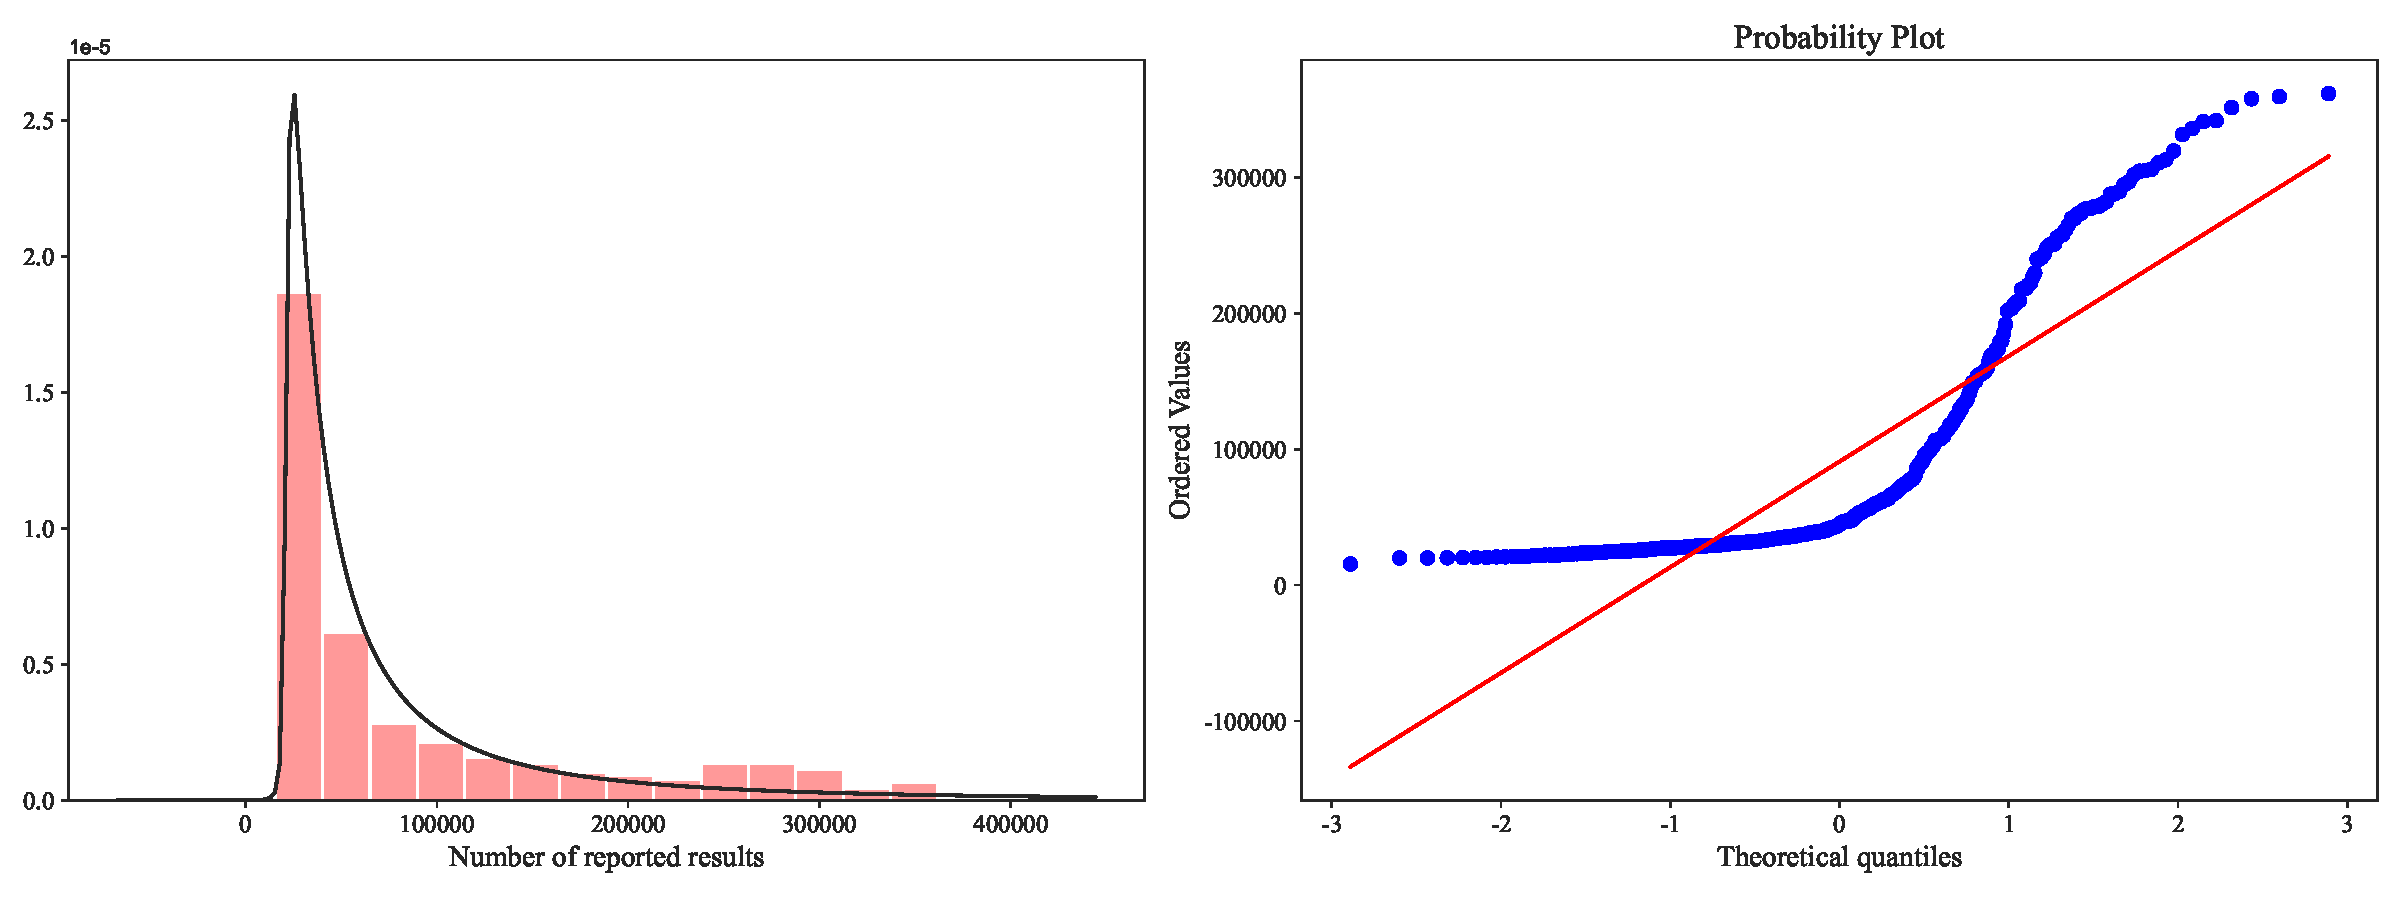
\includegraphics[width=0.90\textwidth]{正态分布分析.pdf}
		\caption{正态分布分析}
		\label{fig:正态分布分析}
	\end{figure}
	
	上图左图描述报告结果数量与频率的关系,发现报告结果数量主要集中在$20000$附近,位于其他区间的报告结果数量出现的频率很小。右图描述了样本分位数与观测值确实服从正态分布时所观察到的分位数之间的关系,当各点近似分布在一条直线附近时,可认为正态性假设成立。而图中点连成的曲线与直线存在很大偏差,故人数不符合正态分布。因此我们有理由认为对于该数据集,进行线性回归分析可能会在一定程度上得到较优效果,但这并不是在数据集集中部分的效果,极有可能会对未来的预测产生较大误差,因此我们考虑建立\textbf{极端梯度提升(eXtreme Gradient Boosting,XGBoost)}模型,首先对每日报告总人数进行预测,再对选择困难模式人数进行预测分析。
	XGBoost算法是一种基于树模型的优化模型,该算法通过多次迭代,生成一个新的树模型用于优化前一个树模型,随着迭代次数的增多,该模型的预测精度也会相应提高\textcolor{blue}{\cite{pxgboost1}}。

		记通过数据处理后的数据集特征为$R\left(x_{ij}\right)_{m\times n}$,表示其包含$m$天的游戏情况,$n$个特征,在训练中形成的CART树的集合记为$F=\left\{f\left(x\right)=w_{q\left(x\right)},q:\mathbf{R}^n\to T,w\in \mathbf{R}^T\right\}$,其中$q$为树模型的叶节点决策规划,$T$为某一树模型叶节点数量,$w$为叶节点对应的得分\textcolor{blue}{\cite{pxgboost2}}。对于预测的$y$值,即$\hat{y}$,计算公式为
		\begin{equation}
			\hat{y}=\varphi \left( x_i \right) =\sum\limits_{k=1}^K{f_k\left( x_i \right)} \label{fXGBoostypre}
		\end{equation}
	
		XGBoost算法在每一次迭代过程中会保存前面所学习的模型,会将这些模型加入到新一轮迭代过程中,因此我们记第$i$个模型为预测结果为
		\begin{equation}
			\hat{y}_{i}^{\left(t\right)}=\hat{y}_{i}^{\left(t-1\right)}+f_t\left(x_i\right) \label{fXGBoostyprei}
		\end{equation}
		
		XGBoost算法的目标函数计算公式如下
		\begin{equation}
			L^{\left(t\right)}=\sum\limits_{i=1}^{n}l\left(y_i,\hat{y}_{i}^{\left(t-1\right)}+f_t\left(x_i\right)\right)+\gamma T+\frac{1}{2}\lambda\sum\limits_{j=1}^T{w_j^2}+\mathrm{const} \label{fXGBoostL}
		\end{equation}
		上述公式中,$l$为模型误差损失,描述在该模型下预测值与实际值之间的出差异损失,$\Omega$为模型叶节点的正则项惩罚系数,$\gamma$与$\lambda$为模型的超参数\textcolor{blue}{\cite{pxgboost2}}。
		
		通常情况下,我们难以用枚举法得到在模型中所训练出来的树结构,因此这里采用贪婪算法,从单叶子节点开始,通过迭代方法,将其加入到树结构中,从而得到最优解,其计算公式\textcolor{blue}{\cite{pxgboost3}}如下
		\begin{equation}
			\mathcal{L}_{split}=\frac{1}{2}\left[\frac{\left(\sum_{i\in I_L}g_i\right)^2}{\sum_{i\in I_L}h_i+\lambda}+\frac{\left(\sum_{i\in I_R}g_i\right)^2}{\sum_{i\in I_R}h_i+\lambda}-\frac{\left(\sum_{i\in I}g_i\right)^2}{\sum_{i\in I}h_i+\lambda}\right]-\gamma \label{fXGBoostLsplit}
		\end{equation}
		其中$I_j=\left\{i|q\left(x_i\right)=j\right\}$为叶节点$j$上的样本集合\textcolor{blue}{\cite{pxgboost2}},且有
		\begin{equation}
			g_i=\partial_{\hat{y}^{\left(t-1\right)}}l\left(y_i,\hat{y}_i^{\left(t-1\right)}\right)
		\end{equation}
		\begin{equation}
			h_i=\partial_{\hat{y}^{\left(t-1\right)}}^2l\left(y_i,\hat{y}_i^{\left(t-1\right)}\right)
		\end{equation}

	\subsubsection{预测2023年5月15日数据}
	依据上述分析,我们首先以报告结果总人数为预测目标,再以报告选择困难模式玩家人数为预测目标对数据集进行训练以及测试\textcolor{blue}{\footnote{对于报告结果总人数预测,我们仅传入游戏编号序列作为自变量;对于报告结果选择困难模式人数预测,我们传入游戏编号及总人数序列作为自变量。}}。划分训练集及测试集比例为$9:1$,通过XGBoost算法对训练集进行训练,同时在测试集上进行评估。我们得到训练测试拟合图,见\textcolor{blue}{\cref{fig:XGBoost预测结果总人数}}及\textcolor{blue}{\cref{fig:XGBoost预测结果困难人数}}。

	\begin{figure}[H]
		\centering
		\begin{minipage}{0.48\linewidth}
			\centering
			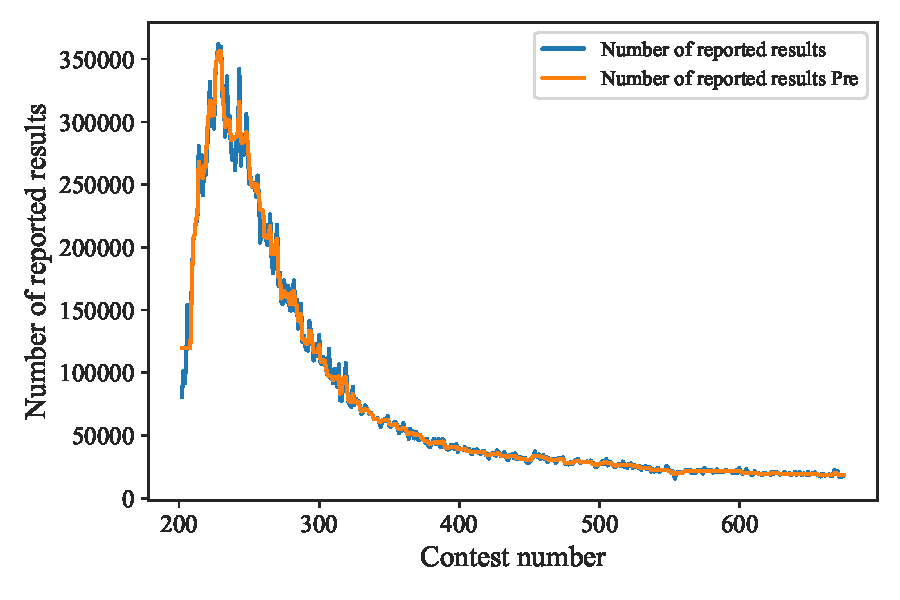
\includegraphics[width=0.80\linewidth]{XGBoost预测结果(总人数).pdf}
			\caption{XGBoost预测结果-总人数}
			\label{fig:XGBoost预测结果总人数}
		\end{minipage}
		%\qquad
		\begin{minipage}{0.48\linewidth}
			\centering
			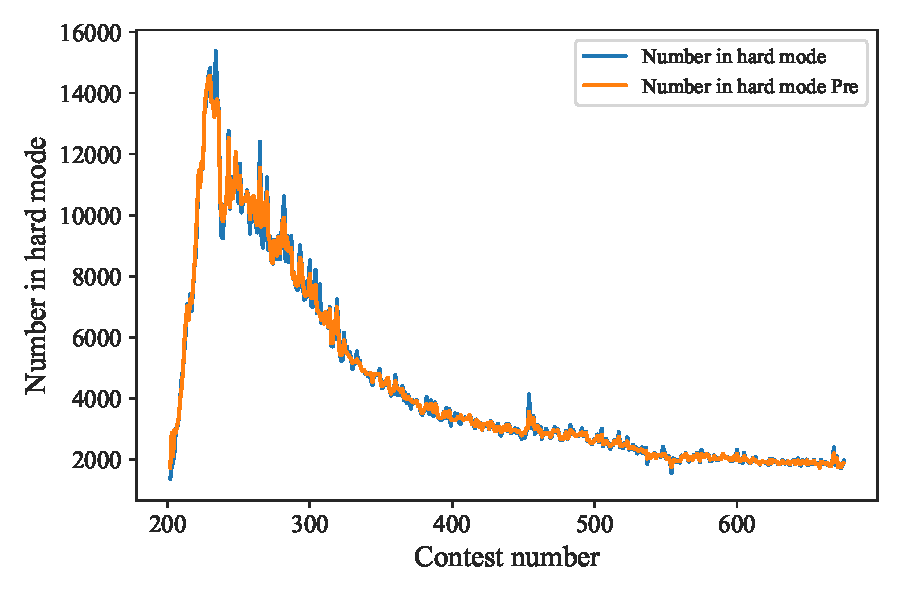
\includegraphics[width=0.80\linewidth]{XGBoost预测结果(困难人数).pdf}
			\caption{XGBoost预测结果-困难人数}
			\label{fig:XGBoost预测结果困难人数}
		\end{minipage}
	\end{figure}
	同时我们还绘制上述两个模型的预测误差图,见\textcolor{blue}{\cref{fig:XGBoost预测误差总人数}}及\textcolor{blue}{\cref{fig:XGBoost预测误差困难人数}}。

	\begin{figure}[H]
		\centering
		\begin{minipage}{0.48\linewidth}
			\centering
			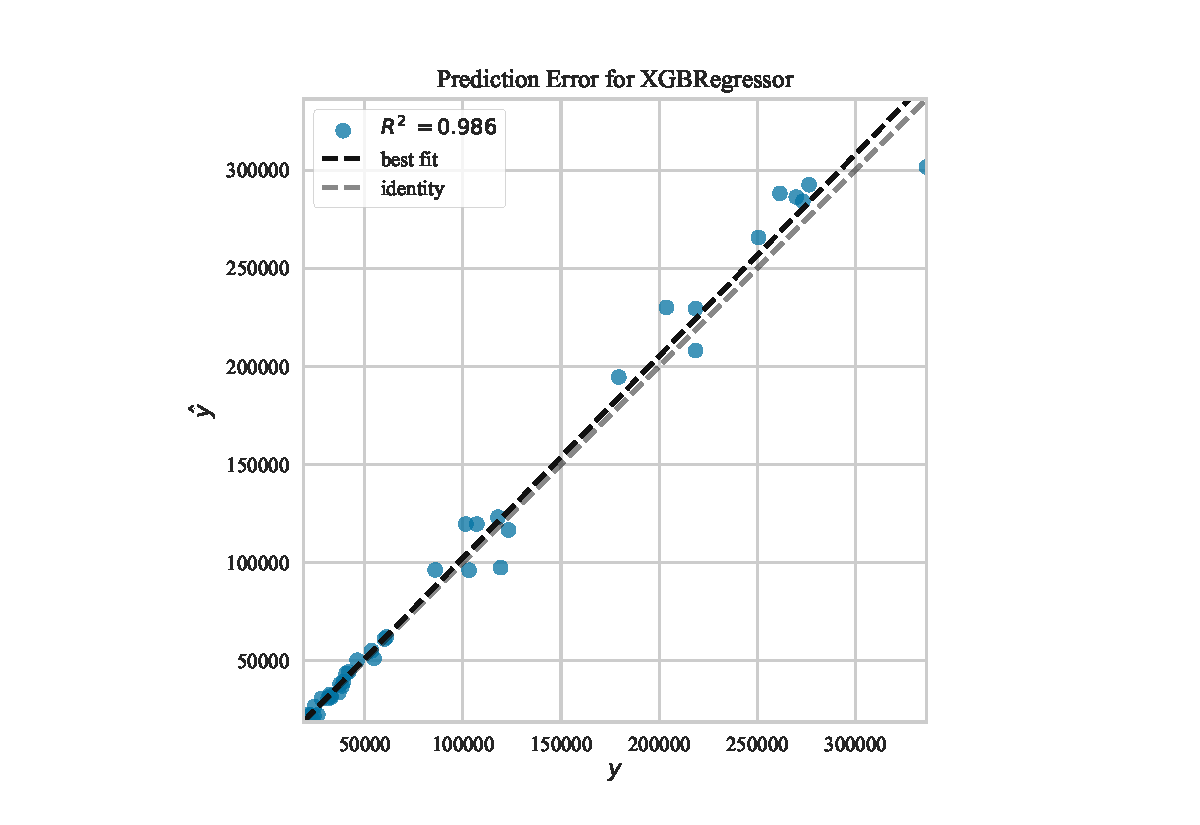
\includegraphics[width=0.6\linewidth]{XGBoost预测误差(总人数).pdf}
			\caption{XGBoost预测误差-总人数}
			\label{fig:XGBoost预测误差总人数}
		\end{minipage}
		%\qquad
		\begin{minipage}{0.48\linewidth}
			\centering
			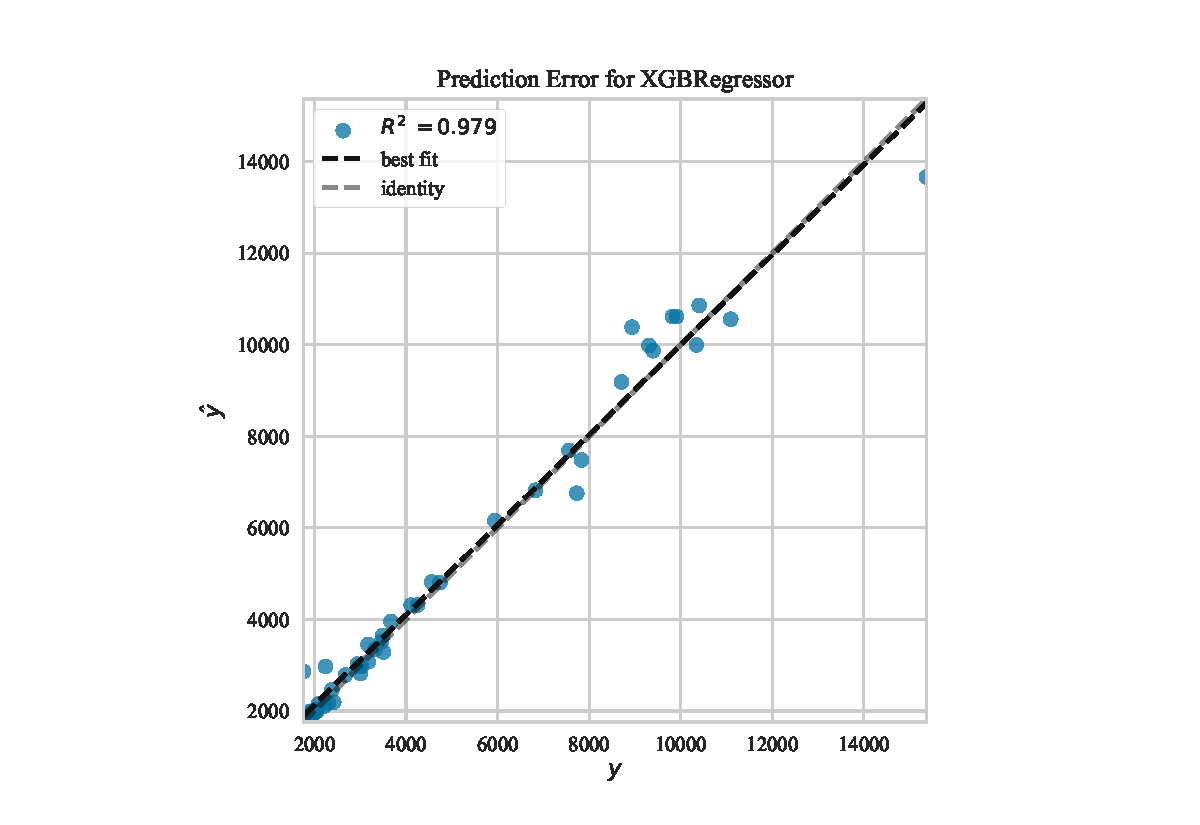
\includegraphics[width=0.6\linewidth]{XGBoost预测误差(困难人数).pdf}
			\caption{XGBoost预测误差-困难人数}
			\label{fig:XGBoost预测误差困难人数}
		\end{minipage}
	\end{figure}
	此外,我们还计算出模型的\textbf{平均绝对误差(Mean Absolute Error,MAE)}、\textbf{均方误差(Mean Squared Error,MSE)}、\textbf{均方根误差(Root Mean Squared Error,RMSE)},以及\textbf{拟合优度(Goodness of Fit)}即$\boldsymbol{R^2}$,最终计算结果见\textcolor{blue}{\cref{tab:XGBoost预测结果}}。
	\begin{itemize}
		\item \textbf{平均绝对误差}
			\begin{equation}
			\mathrm{MAE}=\frac{1}{n}\sum_{i=1}^{n}\left|y_{i}-\hat{y}_{i}\right| \label{MAE}
			\end{equation}
		\item \textbf{均方误差}
			\begin{equation}
			\mathrm{MSE}=\frac{1}{n}\sum_{i=1}^{n}\left(y_{i}-\hat{y}_{i}\right)^{2} \label{MSE}
			\end{equation}
		\item \textbf{均方根误差}
			\begin{equation}
			\mathrm{RMSE}=\sqrt{\text{MSE}} \label{RMSE}
			\end{equation}
		\item \textbf{拟合优度}$\boldsymbol{R^2}$
			\begin{equation}
			R^{2}=\frac{\sum\limits_{i=1}^{n}\left(\hat{y}_{i}-\overline{y}\right)^{2}}{\sum\limits_{i=1}^{n}\left(y_{i}-\overline{y}\right)^{2}} \label{R2}
			\end{equation}
	\end{itemize}
  
根据\textcolor{blue}{\cref{tab:XGBoost预测结果}}结果,我们可以发现XGBoost回归预测对于该数据集有较优表现,在误差允许范围内,预测效果良好。
\begin{table}[H]
	\centering
	\caption{XGBoost回归预测结果}
	\scalebox{0.85}{
	  \begin{tabular}{ccccc}
	  \toprule
	  \textbf{预测类别} & \textbf{MAE} & \textbf{MSE} & \textbf{RMSE} & $\boldsymbol{R^2}$ \\
	  \midrule
	  总人数   & 2586  & 29849352 & 5463  & 0.9957 \\
	  选择困难游戏模式人数  & 97    & 38334 & 196   & 0.9959 \\
	  \bottomrule
	  \end{tabular}}
	\label{tab:XGBoost预测结果}
\end{table}

现我们将对2023年5月15日报告情况进行预测,并且为使分析更具有一般性,我们给出在$95\,\%$的置信水平下的预测区间。但在上述分析中,我们发现对于每日报告的人数并不服从正态分布,这是由于我们选取Wordle从发布至今的每日人数情况进行分析,但游戏从发布至今存在增长、成熟、衰退与稳定的时期。根据\textcolor{blue}{\cref{fig:XGBoost预测结果总人数}}及\textcolor{blue}{\cref{fig:XGBoost预测结果困难人数}}所示结果,我们可以发现从2022年6月开始,Wordle的人数逐渐进入稳定期,对于该时期的数据我们有理由认为其每日报告的人数服从正态分布。因此我们可以利用\textcolor{blue}{\cref{tab:XGBoost预测结果}}中的RMSE来计算预测区间,其计算方式如下:

记每日报告人数为$X$,则$X\sim N(\mu,\sigma^2)$,其中$\mu$为样本均值,这里由于处于稳定期,我们假设预测值近似为样本均值,$\sigma$为RMSE,则标准误差为
\begin{equation}
	\text{SE}=\frac{\sigma}{\sqrt{n}}=\frac{\text{RMSE}}{\sqrt{n}}
\end{equation}
其中$n$为样本总量。这里我们设定预测区间为$95\,\%$的置信水平,则有
\begin{equation}
	P(\mu-2\cdot\text{SE} < X < \mu+2\cdot\text{SE})=0.95
\end{equation}
因此在$95\,\%$的置信水平下的预测区间为
\begin{equation}
	\left[\mu-2\sigma,\mu+2\sigma\right]
\end{equation}

通过上述分析,预测具体结果见\textcolor{blue}{\cref{tab:2023年5月15日报告情况预测}}。
\begin{table}[H]
	\centering
	\caption{2023年5月15日报告情况预测结果}
	\scalebox{0.85}{
	  \begin{tabular}{cccccc}
	  \toprule
	  \textbf{预测类别} & \textbf{预测值} & \textbf{RMSE} & \textbf{SE} & \textbf{区间下界} & \textbf{区间上界} \\
	  \midrule
	  总人数   & 18334 & 5463  & 251   & 17831  & 18352  \\
	  选择困难游戏模式人数  & 1874  & 196   & 9     & 1856  & 1892  \\
	  \bottomrule
	  \end{tabular}}
	\label{tab:2023年5月15日报告情况预测}
\end{table}

因此,我们得到最终预测结果,即2023年5月15日的报告情况为:报告总人数为$\left[17831,18352\right]$人,选择困难模式游戏的人数为$\left[1856,1892\right]$人。
	\subsubsection{单词属性分析}
	在Wordle游戏中,影响玩家猜测次数的因素包括单词结构的复杂性、单词使用频率、词性等相关因素。为了区分不同单词对猜谜游戏难度的影响,我们通过分析以下属性对单词进行量化。
\begin{itemize}
	\item \textbf{单词组合}:单词组合我们也可以理解为Wordle谜底的五个字母长度的单词每一位置上的字母,不同的字母可能会组成不同的词根词缀,从而影响到玩家猜词的次数。
	\item \textbf{单词每位字母在英文常用词汇中出现的频率}:单词在每一位上的字母在英文常用词汇中有着不同的出现频率,从而每一个单词自身所携带的信息熵也有所不同。频率低的字母组成的单词在常用词中通常也出现频率较低,即会导致该词流行度较低,比如字母“E”,其词频较高,则由其组成的单词基数较大,从而其不确定性较高,因此玩家可能难以想出该词,从而影响到玩家猜词的次数。
	\item \textbf{单词中元音字母个数}:在英文26个字母中,元音字母为“a”“e”i”“o”“u”。单词中元音字母越多,发音可能也就越难,从而在一定程度上会影响到该词的难度。
	\item \textbf{单词词性}:不同的英文单词有着不同的词性,如名词、动词、形容词、副词、介词等。不同词性的单词会影响到玩家对该词的认知,同时,部分单词还有着多种词性,这也会在一定程度上影响玩家猜词情况。因此这里我们为了高效且准确地分析单词词性,我们选择Python中的nltk库\textcolor{blue}{\footnote{nltk是Python中著名的自然语言处理(Natural Language Processing,NLP)第三方库}}进行词性标注。通过该库,我们统计出数据集中单词属性的结果,见\textcolor{blue}{\cref{tab:单词词性分析}}。
\begin{table}[H]
	\centering
	\caption{单词词性分析}
	\scalebox{0.90}{
	  \begin{tabular}{cccc}
	  \toprule
	  \textbf{简称} & \textbf{描述} & \textbf{中文释义} & \textbf{个数} \\
	  \midrule
	  NN    & noun singular & 名词单数  & 274 \\
	  JJ    & adjective & 形容词   & 110 \\
	  VBP   & the present tense of the non-third person singular & 非第三人称单数的现在时 & 16 \\
	  VBD   & past tense & 过去时   & 14 \\
	  RB    & adverb & 副词    & 14 \\
	  VB    & verb prototype & 动词原型  & 8 \\
	  NNS   & noun plural & 名词的复数 & 7 \\
	  VBN   & past participle of verb & 动词过去分词 & 6 \\
	  IN    & a preposition or subordinate conjunction & 介词或从属连词 & 5 \\
	  VBZ   & third person singular present tense & 第三人称单数现在时 & 3 \\
	  VBG   & gerund or present participle & 动名词或现在分词 & 3 \\
	  DT    & qualifier & 修饰词   & 2 \\
	  CC    & joint conjunction & 连词 & 2 \\
	  JJR   & comparative adjective & 比较性形容词 & 2 \\
	  MD    & modal verb & 情态助动词 & 2 \\
	  PRP\$ & possessive pronoun & 物主代词  & 1 \\
	  JJS   & superlative adjective & 形容词最高级 & 1 \\
	  RBR   & comparative adverb & 比较副词  & 1 \\
	  WRB   & wh-verb & 疑问词   & 1 \\
	  \bottomrule
	  \end{tabular}}
	\label{tab:单词词性分析}
\end{table}
  
	\item \textbf{单词中重复字母个数}:不同的单词其字母可能存在重复现象,如单词“GOOD”,字母“O”重复,对于Wordle游戏而言,程序不会提示玩家在游戏谜底中是否存在重复的字母。为了规范统计,我们进行以下定义:
	\begin{itemize}
		\item {\heiti 重复字母个数为0}:单词中不存在重复的字母,即每一位单词均不一致,例如单词“SMART”;
		\item {\heiti 重复字母个数为2}:单词中有一个字母重复,由于重复至少存在两个相同字母,例如单词“SPELL”;
		\item {\heiti 重复字母个数为3}:例如单词“EERIE”;
		\item {\heiti 重复字母个数为4}:例如单词“AMASS”。
	\end{itemize}
\end{itemize}

因此,经过上述分析,我们可以构造出以下列数据:
	\begin{itemize}
		\item {\heiti 单词每位字母}:由于单词长度为五个字母,因此存在五列,构造如下
		$$
		\left[\text{w1}\quad \text{w2}\quad \text{w3}\quad \text{w4}\quad \text{w5}\right]
		$$
		\item {\heiti 单词每位字母频率}:利用Map与字典配对,与每位字母形成键值对,构造如下
		$$
		\left[\text{w1\_fre}\quad\text{w2\_fre}\quad\text{w3\_fre}\quad\text{w4\_fre}\quad\text{w5\_fre}\right]
		$$
		\item {\heiti 单词中元音个数}:构造的列名为——$\text{Vowel\_fre}$
		\item {\heiti 单词中辅音个数}:构造的列名为——$\text{Consonant\_fre}$
		\item {\heiti 单词词性}:构造的列名为——$\text{Speech}$
		\item {\heiti 单词中重复字母个数}:构造的列名为——$\text{Same\_letter\_fre}$
	\end{itemize}
	
	构造完上述指标后,需要对非数字类型数据编码。对于每位字母,为了避免大写字母的影响,我们首先将所有单词均转化为小写字母组合字母,再将“a”至“z”以数字$1$至$26$连续编号;对于单词词性,我们采用Label Encoder编码。
	\subsubsection{单词属性与玩家游戏中的表现关联分析}\label{单词属性与玩家游戏中的表现关联分析}
	对数据集经过上述单词属性的分析,我们将其与玩家游戏中的表现进行关联分析,这里我们绘制\textbf{皮尔逊相关系数(Pearson Correlation Coefficient)}热力图,如\textcolor{blue}{\cref{fig:皮尔逊相关系数热力图}}所示,其可衡量两个变量之间的相似度\textcolor{blue}{\cite{ppearson1}},不妨用$\rho\left(x,y\right)$表示皮尔逊相关系数,则
	\begin{equation}
	\rho\left(x,y\right)=\frac{\sum\limits_{i=1}^{n}\left(x_{i}-\mu_x\right)\left(y_{i}-\mu_y\right)}{\sqrt{\sum\limits_{i=1}^{n}\left(x_{i}-\mu_x\right)^{2}}\sqrt{\sum\limits_{i=1}^{n}\left(y_{i}-\mu_y\right)^{2}}},\quad\mu=\frac{1}{m}\sum_{i=1}^{m}x_i \label{fpearson}
	\end{equation}
	其中,$n$为数据维度,$m$为数据个数。
	
	由该定义,显然$\rho\in[-1,1]$。当$\rho>0$时,上述两变量呈正相关;当$\rho=0$时,上述两变量不相关;当$\rho<0$时,上述两变量呈负相关。当$\left|\rho\right|$越接近于$1$时,则上述两变量相关性就越强\textcolor{blue}{\cite{ppearson2}}。
	\begin{figure}[H]
		\centering
		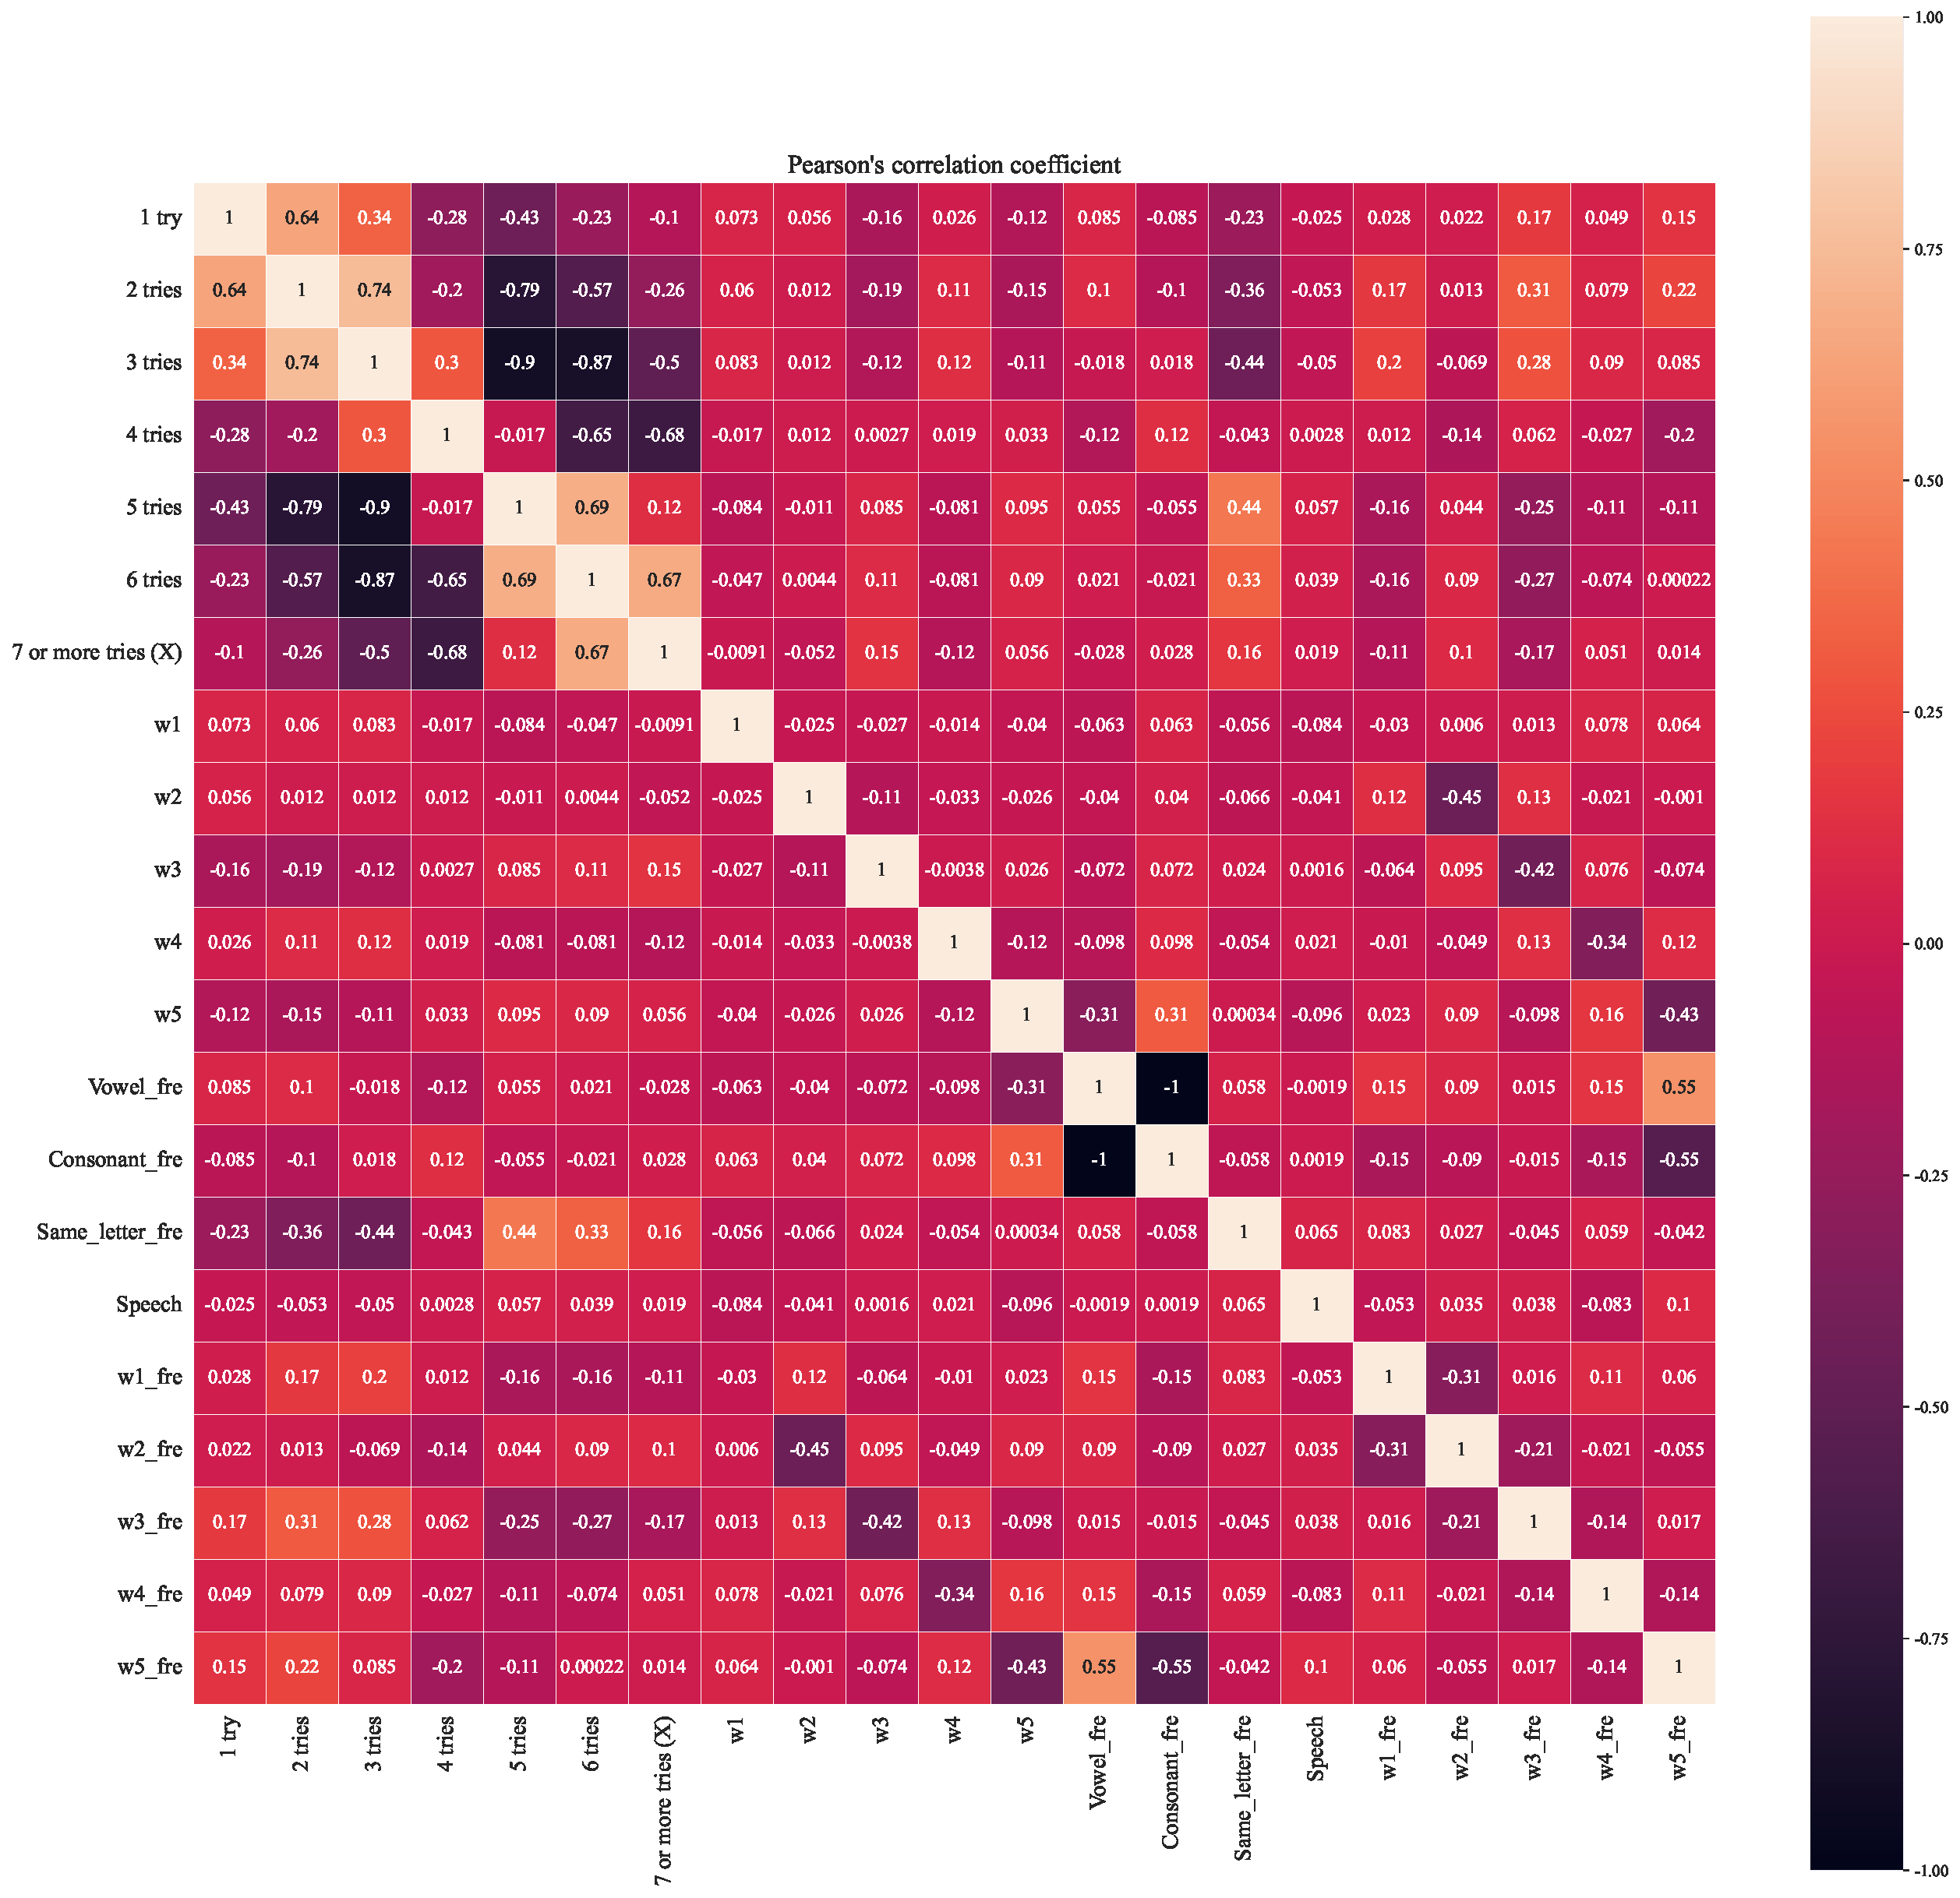
\includegraphics[width=1.0\textwidth]{皮尔逊相关系数.pdf}
		\caption{皮尔逊相关系数热力图}
		\label{fig:皮尔逊相关系数热力图}
	\end{figure}

	由皮尔逊相关系数热力图可以发现,词频与前三次尝试有显著的正相关关系,而与后几次尝试呈负相关。由此看出当一个词的词频增加时,玩家可能在前三次猜测中猜中该词,也表明该词较为简单。字母重复数与前三次尝试呈负相关,与后几次尝试呈正相关,这表明一个词中出现的重复字母越多,玩家越难以较少的次数完成猜词。同时我们也发现元音、辅音和词性对猜词次数的影响较小。同时,我们还发现在困难模式下,由于玩家只能使用前面所尝试的正确单词,因此在后续猜词中,玩家可选词语将减少,若不进行词语检索,那么将增加游戏难度,此外,也有一定可能将减少玩家猜测次数,将再更少次数内猜中该词。因此在困难模式下,得分百分比情况可能会导致峰值有左偏或有一定右偏趋势。

	\subsection{问题二模型的建立与求解}
	对于该问题,我们需要完成以下几点任务:
	\begin{itemize}
		\item 对于给定的单词,我们需要建立相关模型,预测在当天玩家游戏最终结果的尝试次数的百分比分布;
		\item 分析模型的不确定性因素。
	\end{itemize}
	
	因此,我们需要根据相关回归算法,以单词属性为主要特征,对给定的单词玩家当日进行不同尝试次数的百分比进行预测,同时我们还需要对模型进行效果分析,并解释模型的不确定性因素。
	\subsubsection{模型的分析}
	我们综合XGboost回归,线性回归,随机森林回归,LightGBM回归预测模型分析,以选择最优的算法进行预测。同时我们将使用以下指标进行评价:均方误差(MSE),平均绝对误差(MAE),均方根误差(RMSE),拟合优度$R^2$。对于该题,我们划分自变量及因变量如下:
	\begin{itemize}
		\item \textbf{因变量}:玩家当日猜词尝试次数的百分比分布,对应于数据集
		$$
		\left[1\,\text{try}\quad2\,\text{tries}\quad3\,\text{tries}\quad4\,\text{tries}\quad5\,\text{tries}\quad6\,\text{tries}\quad7\,\text{or more tries (X)}\right]
		$$
		\item \textbf{自变量}:
		\begin{itemize}
			\item {\heiti 竞赛编号}:$\text{Contest number}$
			\item {\heiti 每日报告总人数}:$\text{Number of reported results}$
			\item {\heiti 每日报告选择困难模式的人数}:$\text{Number in hard mode}$
			\item {\heiti 单词每位字母}:$\left[\text{w1}\quad \text{w2}\quad \text{w3}\quad \text{w4}\quad \text{w5}\right]$
			\item {\heiti 单词每位字母频率}:$\left[\text{w1\_fre}\quad\text{w2\_fre}\quad\text{w3\_fre}\quad\text{w4\_fre}\quad\text{w5\_fre}\right]$
			\item {\heiti 单词中元音个数}:$\text{Vowel\_fre}$
			\item {\heiti 单词中辅音个数}:$\text{Consonant\_fre}$
			\item {\heiti 单词词性}:$\text{Speech}$
			\item {\heiti 单词中重复字母个数}:$\text{Same\_letter\_fre}$
		\end{itemize}
		
	\end{itemize}
	
	根据上述划分,同时我们划分训练集及测试集比例为$9:1$,通过Python编程,我们得到上述各模型对于不同尝试次数的各项指标,最终结果见\textcolor{blue}{\cref{tab:回归模型指标}}。分析该表,我们可以发现四种模型中,XGBoost及随机森林效果较优秀,其MSE、RMSE、MAE均较小,$R^2$接近于$1$,说明模型的拟合效果较好。而LightGBM与线性回归模型效果较差。因此这里我们初步选择XGBoost及随机森林作为我们的预测模型。

\begin{table}[H]
	\centering
	\caption{多种回归模型预测指标}
	\setlength{\aboverulesep}{0pt}
	\setlength{\belowrulesep}{0pt}
	\scalebox{0.86}{
	  \begin{tabular}{c|cccc||cccc}
	  \toprule
	  \multirow{2}[2]{*}{\textbf{尝试次数}} & \multicolumn{4}{c||}{\textbf{线性回归}} & \multicolumn{4}{c}{\textbf{XGBoost}} \\
			& \textbf{MSE} & \textbf{RMSE} & \textbf{MAE} & $\boldsymbol{R^2}$ & \textbf{MSE} & \textbf{RMSE} & \textbf{MAE} & $\boldsymbol{R^2}$ \\
	  \midrule
	  1     & 0.4272  & 0.6536  & 0.4182  & 0.2258  & 0.0950  & 0.3083  & 0.0573  & 0.8278  \\
	  2     & 10.3890  & 3.2232  & 2.3802  & 0.3729  & 0.6521  & 0.8075  & 0.2110  & 0.9606  \\
	  3     & 35.9825  & 5.9985  & 4.8689  & 0.4075  & 3.5164  & 1.8752  & 0.5038  & 0.9421  \\
	  4     & 24.2460  & 4.9240  & 3.8189  & 0.1474  & 1.6169  & 1.2716  & 0.3542  & 0.9431  \\
	  5     & 21.6561  & 4.6536  & 3.7722  & 0.3944  & 1.7603  & 1.3268  & 0.3684  & 0.9508  \\
	  6     & 25.4959  & 5.0493  & 3.9937  & 0.2920  & 1.8777  & 1.3703  & 0.3563  & 0.9479  \\
	  X     & 13.8710  & 3.7244  & 2.1373  & 0.1172  & 0.7300  & 0.8544  & 0.1744  & 0.9535  \\
	  \midrule
	  \multirow{2}[2]{*}{\textbf{尝试次数}} & \multicolumn{4}{c||}{\textbf{随机森林}} & \multicolumn{4}{c}{\textbf{LigtGBM}} \\
			& \textbf{MSE} & \textbf{RMSE} & \textbf{MAE} & $\boldsymbol{R^2}$ & \textbf{MSE} & \textbf{RMSE} & \textbf{MAE} & $\boldsymbol{R^2}$ \\
	  \midrule
	  1     & 0.1394  & 0.3734  & 0.1847  & 0.7473  & 0.3848  & 0.6203  & 0.3868  & 0.3026  \\
	  2     & 2.0268  & 1.4237  & 1.0015  & 0.8777  & 8.9184  & 2.9864  & 2.1563  & 0.4617  \\
	  3     & 6.4768  & 2.5450  & 1.9300  & 0.8934  & 29.9229  & 5.4702  & 4.4812  & 0.5073  \\
	  4     & 4.5865  & 2.1416  & 1.4993  & 0.8387  & 18.4182  & 4.2916  & 3.2479  & 0.3524  \\
	  5     & 4.2666  & 2.0656  & 1.5381  & 0.8807  & 18.5074  & 4.3020  & 3.4718  & 0.4824  \\
	  6     & 4.8076  & 2.1926  & 1.5958  & 0.8665  & 20.5757  & 4.5360  & 3.5539  & 0.4287  \\
	  X     & 2.3988  & 1.5488  & 0.8450  & 0.8473  & 11.3648  & 3.3712  & 1.7032  & 0.2767  \\
	  \bottomrule
	  \end{tabular}}
	\label{tab:回归模型指标}
\end{table}

	\subsubsection{XGBoost与随机森林回归分别预测得分百分比结果}
	对于XGBoost回归模型,其原理在\textcolor{blue}{\nameref{XGBoost}}中我们已经分析,此处不再赘述。
	
	这里我们分析随机森林回归,\textbf{随机森林回归(Random Forest Regression,RFR)}是一种采用多个决策树模型来预测分析数据的机器学习算法。它从原始训练集中随机选择一部分样本构成样本子集,使每棵决策树在不同的样本集上训练。在每个子样本集上使用决策树算法构建决策树,并在其生长过程中采用递归选择最佳划分特征,最后通过多棵决策树的预测结果进行加权平均,得到回归结果。算法伪代码如\textcolor{blue}{Algorithm \ref{RFfunction}}所示。

	\scalebox{0.85}{
	\begin{algorithm}[H]
		\label{RFfunction}
		\KwData{数据集$\mathcal{D}$}
		\textbf{function} DTree$\left(\mathcal{D}\right)$\
		
		\eIf{Termination}
		{\textbf{return} $\mathrm{base}\left(g_t\right)$}
		{\textbf{learn} $b\left(x\right)$并且依据$b\left(x\right)$划分$\mathcal{D}$为$\mathcal{D}_C$\

		\textbf{build} $G_C \leftarrow$ DTree($\mathcal{D}_C$)\

		\textbf{return} $G\left(x\right)=\sum\limits_{C=1}^{C}[\![b\left(x\right)=C]\!]G_C\left(x\right)$}
		
		\textbf{function} RandomForest$\left(\mathcal{D}\right)$\
		
		\For{$t=1,2,3,\cdots,T$}{\textbf{request} 数据集$\tilde{\mathcal{D}}_t \leftarrow$ BoostStrapping$\left(\mathcal{D}\right)$\
		
		\textbf{obtain} DTree $g_t\leftarrow$ DTree$\left(\tilde{\mathcal{D}}_t\right)$\

		\textbf{return} $G=$ Uniform$\left(g_t\right)$
		}
		
		\KwResult{随机森林模型$G=\mathrm{Uniform}\left(g_t\right)$}
		\caption{随机森林(Random Forest)}
	\end{algorithm}}

	我们在原数据集上进行训练模型,再将单词“EERIE”构造出相同指标,进行预测。其中2023年5月15日报告总人数及选择困难人数我们利用问题一的结果,因此,我们得到关于2023年5月15日,给定的单词“EERIE”的相关特征数据,如\textcolor{blue}{\cref{tab:2023年5月15日EERIE特征数据}}所示。

\begin{table}[H]
	\centering
	\caption{2023年5月15日EERIE特征数据}
	\scalebox{0.80}{
	  \begin{tabular}{ccccc}
	  \toprule
	  \multicolumn{5}{c}{\textbf{EERIE预测特征(自变量)}} \\
	  \midrule
	  \multicolumn{1}{c}{\textbf{Date}} & \textbf{Contest number} & \textbf{Word} & \textbf{Number of reported results} & \textbf{Number in hard mode} \\
	  \midrule
	  \multirow{3}[6]{*}{2023/5/15} & 695   & EERIE & 18334 & 1874 \\
  \cmidrule{2-5}          & \textbf{Vowel\_fre} & \textbf{Speech} & \textbf{Consonant\_fre} & \textbf{Same\_letter\_fre} \\
  \cmidrule{2-5}          & 4     & 7     & 1     & 3 \\
	  \midrule
	  \textbf{w1} & \textbf{w2} & \textbf{w3} & \textbf{w4} & \textbf{w5} \\
	  \midrule
	  5     & 5     & 18    & 9     & 5 \\
	  \midrule
	  \textbf{w1\_fre} & \textbf{w2\_fre} & \textbf{w3\_fre} & \textbf{w4\_fre} & \textbf{w5\_fre} \\
	  \midrule
	  0.1142 & 0.1142 & 0.0751 & 0.0794 & 0.1142 \\
	  \bottomrule
	  \end{tabular}}
	\label{tab:2023年5月15日EERIE特征数据}
\end{table}

	依据上述数据,我们对该日玩家尝试次数百分比进行预测,两模型预测结果及预测结果百分比之和如\textcolor{blue}{\cref{tab:2023年5月15日EERIE预测结果}}所示。

\begin{table}[H]
	\centering
	\caption{2023年5月15日EERIE预测结果}
	\scalebox{0.85}{
	  \begin{tabular}{ccccccccc}
	  \toprule
	  \textbf{模型} & \textbf{1} & \textbf{2} & \textbf{3} & \textbf{4} & \textbf{5} & \textbf{6} & \textbf{X} & \textbf{百分比累计和} \\
	  \midrule
	  XGBoost & 0.1334  & 4.9177  & 15.3803  & 21.7288  & 28.9516  & 16.2925  & 2.3451  & 89.7494  \\
	  随机森林  & 0.1700  & 4.7300  & 16.2400  & 30.7200  & 27.8600  & 14.0300  & 6.0800  & 99.8300  \\
	  \bottomrule
	  \end{tabular}}
	\label{tab:2023年5月15日EERIE预测结果}
\end{table}
  
	\subsubsection{EERIE预测及模型检验}
	通过分析\textcolor{blue}{\cref{tab:回归模型指标}}及\textcolor{blue}{\cref{tab:2023年5月15日EERIE预测结果}},我们可以发现,对于XGBoost而言,其虽然在MSE、RMSE、MAE、$R^2$上有较优表现,但是其对于“EERIE”的预测效果较差,玩家尝试次数情况百分比累加和仅有$89.7494\,\%$不为$100\,\%$,显然该预测结果偏差较大,究其原因,可能是由于模型产生过拟合现象,因此我们放弃XGBoost回归。而对于随机森林回归,我们发现,其在MSE、RMSE、MAE、$R^2$上的表现仅次于XGBoost模型,且预测结果在我们先前分析的百分比累计和为$\left(100\pm2\right)\,\%$的允许误差范围内。

	\begin{figure}[H]
		\centering
		\begin{minipage}{0.48\linewidth}
			\centering
			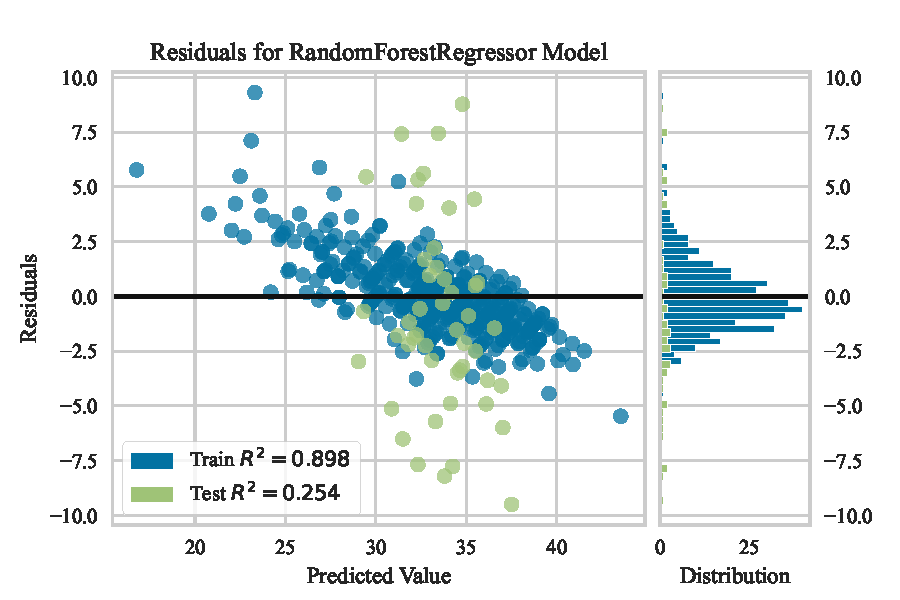
\includegraphics[width=0.95\linewidth]{预测残差图-4.pdf}
			\caption{随机森林预测残差(尝试4次)}
			\label{fig:预测残差图-4}
		\end{minipage}
		%\qquad
		\begin{minipage}{0.48\linewidth}
			\centering
			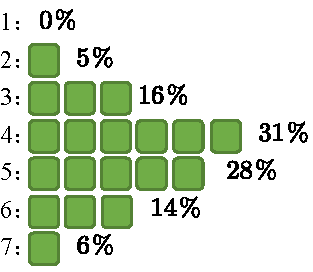
\includegraphics[width=0.74\linewidth]{eerie预测结果.pdf}
			\caption{EERIE预测结果}
			\label{fig:EERIE预测结果}
		\end{minipage}
	\end{figure}

	为讨论模型效果,我们绘制模型的预测残差,这里我们以尝试四次的统计为例,见\textcolor{blue}{\cref{fig:预测残差图-4}}。此外我们还绘制模型平均误差,见\textcolor{blue}{\cref{fig:平均误差}}。
	\begin{figure}[H]
		\centering
		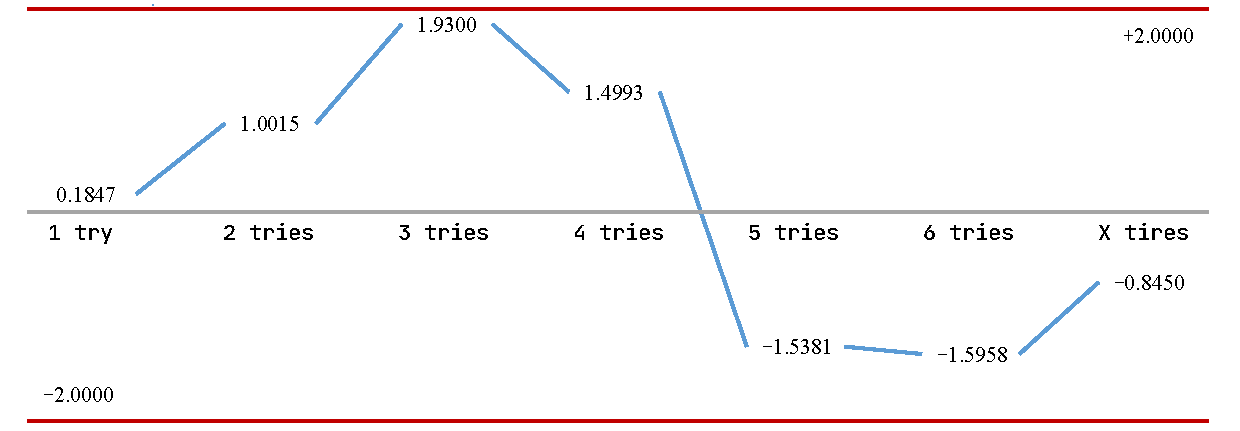
\includegraphics[width=0.80\linewidth]{平均误差.pdf}
		\caption{随机森林回归模型平均误差}
		\label{fig:平均误差}
	\end{figure}

	通过分析上述两幅图,我们可以发现在训练集上该模型拟合优度$R^2$可达到$0.898$,在测试集上拟合优度为$0.254$,这说明该模型在训练集上的拟合效果较好,但是在测试集上的拟合效果较差,这可能是由于一些不确定性因素的影响,我们将在下一小节进行详细分析。同时,我们发现模型对于7次尝试分别均控制在$\pm 2\,\%$之间,这说明模型的预测结果较为稳定,且在误差允许范围内预测结果正确。同时我们结合\textcolor{blue}{\cref{tab:回归模型指标}}中随机森林指标分析,该模型在MSE、RMSE、MAE、$R^2$表现上均较优秀。

	因此我们有理由认为,随机森林模型预测效果较优,且在误差允许范围内预测结果正确。因此,对于2023年5月15日单词“EERIE”的预测结果如\textcolor{blue}{\cref{fig:EERIE预测结果}}所示。

	\subsubsection{不确定性因素分析}\label{不确定性因素分析}
	在随机森林模型的预测过程中,我们考虑了以下可能存在的不确定性:
	\begin{itemize}
		\item 由于样本数据是Wordle玩家自愿在Twitter上发布收集而得到的,考虑到每位玩家的个性,一些玩家可能倾向于发布更好的结果,一些玩家不愿去分享自己较差的结果。因此,收集到的数据存在一定的主观偏差因素,不能保证样本数据的绝对随机性。
		\item 考虑到一种极端的情况,对于部分玩家,可能会使用不同账号,或者使用不同的设备进行游戏,这使得其在第二次游戏时能够一次即可完成挑战,从而影响百分比情况。
		\item 在预测过程中,我们并未对玩家类别进行区分。随着游戏的不断发展,以及老玩家数量的增加,游戏熟练程度的提高可能会导致玩家的平均猜词能力提高。
		\item 对于好友而言,一位玩家成功猜测出词语,其好友极有可能从其处获得提示或答案,从而导致其好友的猜词能力提高,这也可能导致玩家的平均猜词能力提高。
		\item 此外,由于当日词汇的不可预测性,这个词可能会在互联网上流行,从而玩家更容易猜测出该词语,因此我们不能保证模型的绝对优秀,这可能导致预测结果和实际情况之间存在一定的偏差。
	\end{itemize}
	
	\subsection{问题三模型的建立与求解}
	对于该问题,我们需要完成以下几点任务:
	\begin{itemize}
		\item 建立相关模型对附件单词以难度进行分类;
		\item 分析单词的属性与难度之间的关系;
		\item 利用上述模型对单词“EERIE”进行难度分类;
		\item 分析模型的准确性及其他相关指标。
	\end{itemize}

	因此,我们需要建立相关聚类、分类算法,对样本单词进行难度的划分,同时分析单词难度与其对应属性的关系。此外,我们还需要对单词“EERIE”进行难度预测,并讨论模型的准确性。

	\subsubsection{单词聚类、难度分类模型的建立与分析}
	对于单词难度分类,我们首先对单词进行聚类分析,这里我们使用\textbf{K-means聚类(K-means Clustering)}算法\textcolor{blue}{\footnote{在此之前我们考虑过层次聚类(Hierarchical Clustering,HC),且绘制了聚类树状图,但该模型对该数据聚类效果较差,其聚类树状图读者可自行翻阅附录,见\textcolor{blue}{\cref{fig:层次聚类树状图}}.}}。其目的是把目标数据点分成类簇,找到每个簇的中心并使其度量最小化。过程为将数据集聚集成$k$个类簇,从数据集中随机选择$N$个数据点作为数据中心,分别计算出每个点到每个数据中心的距离,并将每个点划分到离最近数据中心的类簇,在数据中心聚集了一些点后,重复上述过程,选出新的数据中心,比较第一次和第二次得到的数据中心,若两个数据中心之间的距离小于某一临界值,则此聚类达到了期望,算法终止,若距离相差很大,则继续执行算法,直到算法终止。
	
	K-means算法首先需要从给定的数据对象中随机指定初始聚类数$k$和相应的初始聚类中心$C$。然后计算从初始聚类中心到其余数据对象的距离。本文选择欧氏距离进行计算。从聚类中心到空间中其他数据对象的欧氏距离公式为:
	\begin{equation}
		d\left(x,C_i\right)=\sqrt{\sum_{j=1}^{m}(x_{j}-C_{ij})^2}
	\end{equation}
	其中$x$为数据对象,$C_i$是第$i$个聚类中心,$m$为数据对象的维度,$x_j$为数据对象$x$的第$j$个维度与聚类中心$C_i$的属性值。

	根据欧氏距离,测量相似度,并将与聚类中心相似度最高的目标数据分配到$C_i$类别。同类化之后,对$k$个聚类中的数据对象进行平均,形成新一轮的聚类中心,从而降低数据集的\textbf{误差平方和(Sum of Square Error,SSE)},其计算公式如下:
	\begin{equation}
		\text{SSE}=\sum_{i=1}^{k}\sum_{x\in C_i}\left|d\left(x,C_i\right)\right|^2
	\end{equation}

	SSE被用来衡量聚类结果的效果。当其不再变化或收敛时,即停止迭代,得到最终结果。

	为了更好地将数据集单词进行聚类,我们需要确定合适的$k$值,因此我们使用肘部法则,绘制肘部法则可视化,确定最适$k$值,如\textcolor{blue}{\cref{fig:肘部法则}}所示。

	\begin{figure}[H]
		\centering
		\begin{minipage}{0.48\linewidth}
			\centering
			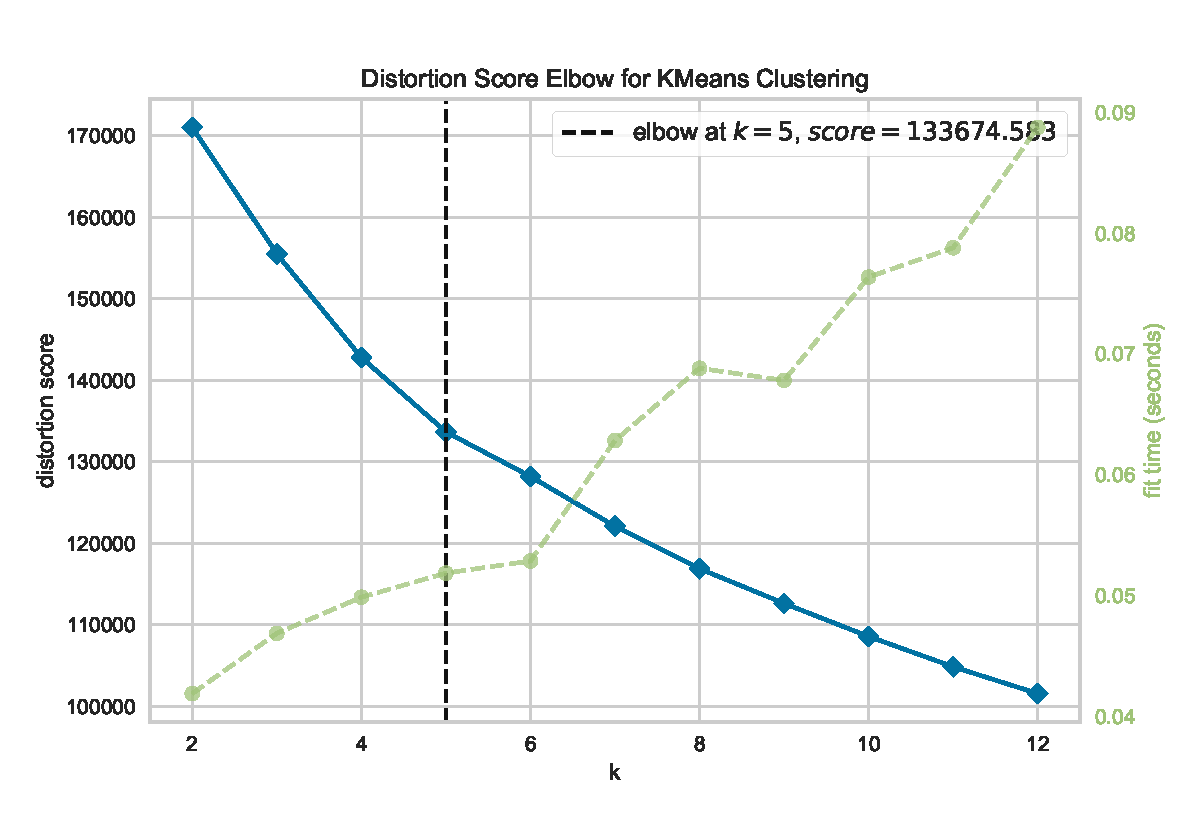
\includegraphics[width=0.98\linewidth]{肘部法则.pdf}
			\caption{肘部法则可视化}
			\label{fig:肘部法则}
		\end{minipage}
		%\qquad
		\begin{minipage}{0.48\linewidth}
			\centering
			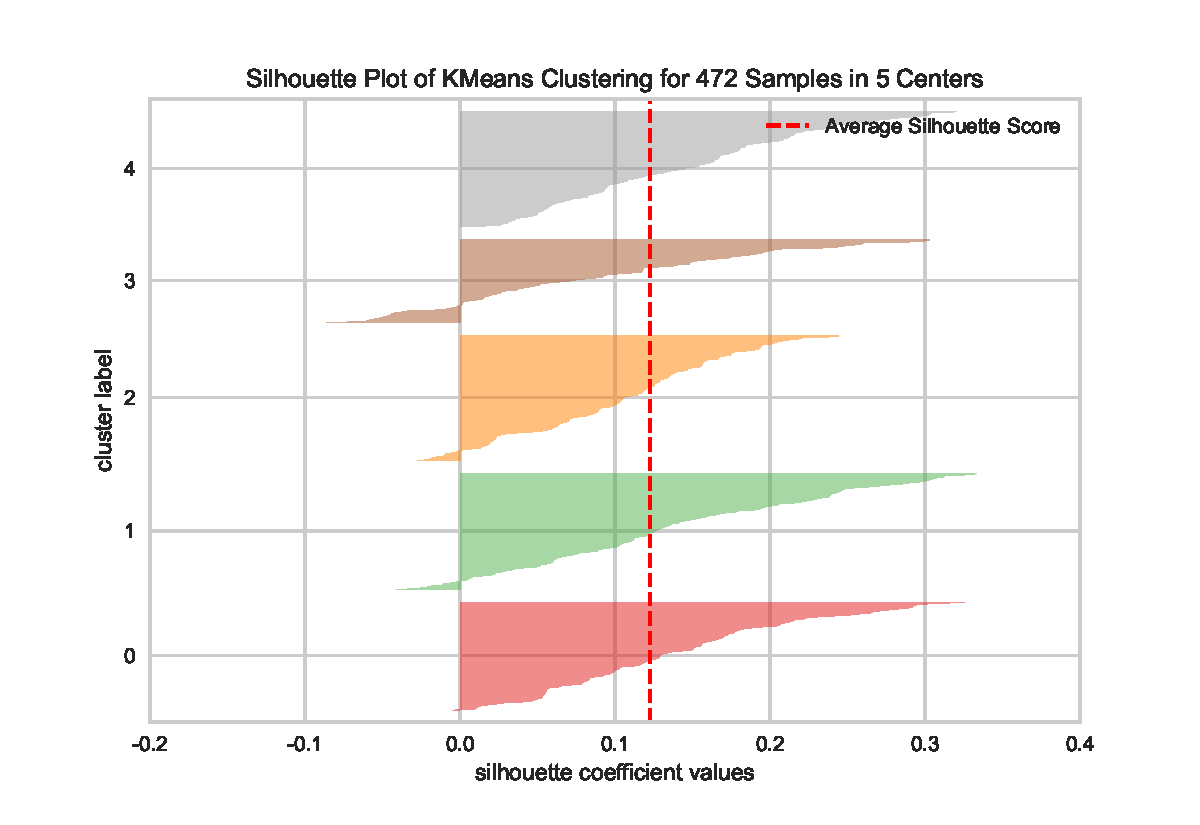
\includegraphics[width=0.98\linewidth]{轮廓系数.pdf}
			\caption{轮廓系数可视化}
			\label{fig:轮廓系数}
		\end{minipage}
	\end{figure}

	根据上图,我们可以选择出最适$k$值,即$k=5$,对应得分为$133674.583$。根据上述结果,我们得到每一个单词所属类别,但此时类别为$0\sim4$编号,因此,我们需要综合分析上述5类单词的难易程度。首先我们定义5个类别难易程度分别为:非常困难(Very Hard)、困难(Hard)、中等(Medium)、容易(Easy)、非常容易(Very Easy)。通过对数据集单词及其属性的综合分析,我们对单词难度进行量化分析,最终确定类别与难度的对应关系,见\textcolor{blue}{\cref{tab:类别与难度的对应关系}}。

\begin{table}[H]
	\centering
	\caption{类别与难度的对应关系}
	\scalebox{0.85}{
	  \begin{tabular}{c|ccccc}
	  \toprule
	  \textbf{类别} & \textbf{0} & \textbf{1} & \textbf{2} & \textbf{3} & \textbf{4} \\
	  \midrule
	  \textbf{难度} & Medium & Very Easy & Hard  & Very Hard & Easy \\
	  \bottomrule
	  \end{tabular}}
	\label{tab:类别与难度的对应关系}
\end{table}

	得到各组别后,我们通过利用\textbf{主成分分析(Principal Component Analysis Cumulative,PCA)}对指标进行降维处理,绘制聚类散点图,如\textcolor{blue}{\cref{fig:聚类散点二维可视化}}及\textcolor{blue}{\cref{fig:聚类散点三维可视化}}所示。
	
	\begin{figure}[H]
		\centering
		\begin{minipage}{0.48\linewidth}
			\centering
			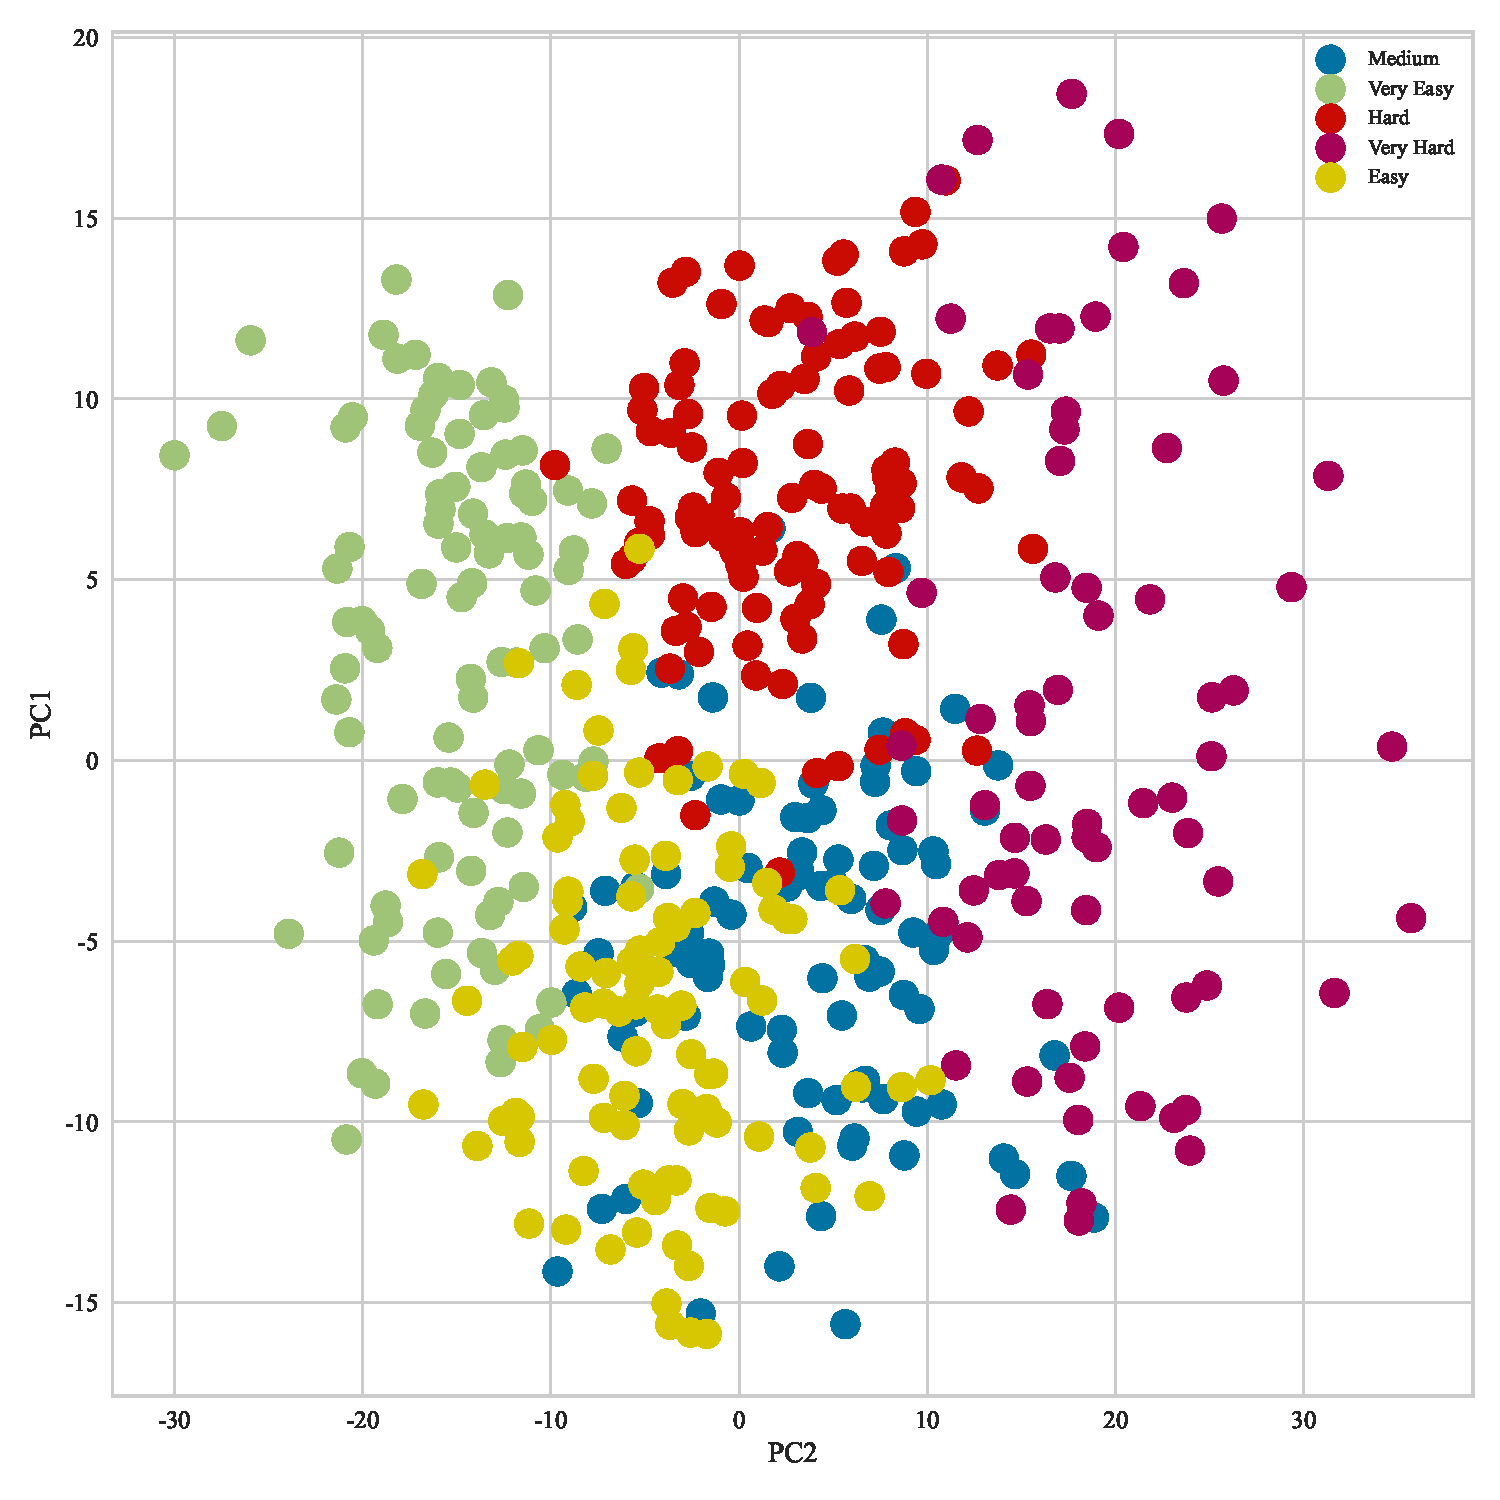
\includegraphics[width=0.80\linewidth]{聚类散点图.pdf}
			\caption{聚类散点二维可视化}
			\label{fig:聚类散点二维可视化}
		\end{minipage}
		%\qquad
		\begin{minipage}{0.48\linewidth}
			\centering
			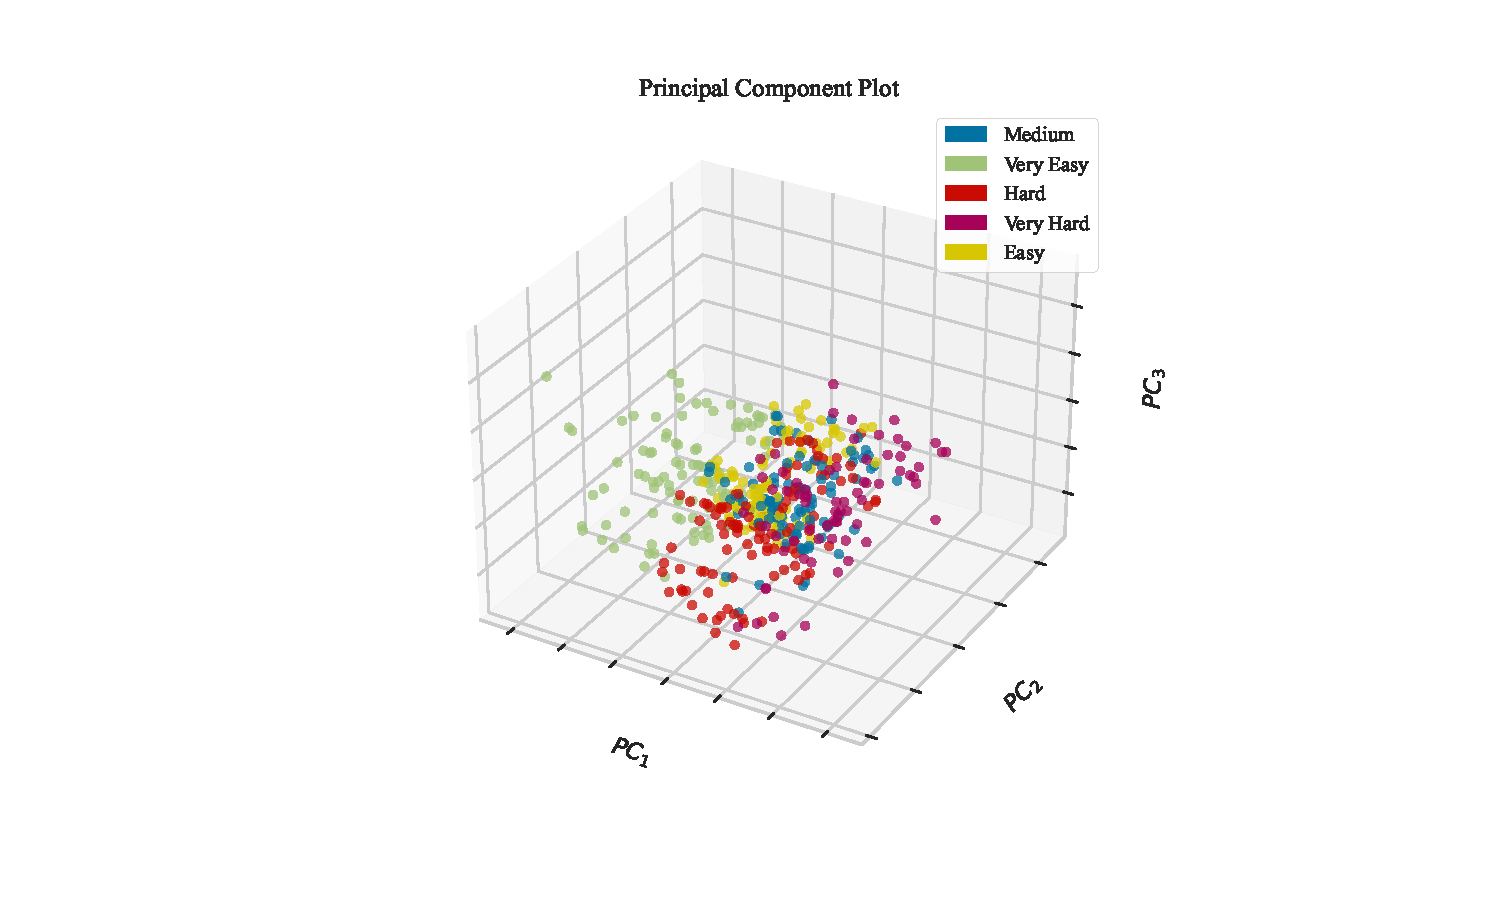
\includegraphics[width=0.81\linewidth]{PCA-3.pdf}
			\caption{聚类散点三维可视化}
			\label{fig:聚类散点三维可视化}
		\end{minipage}
	\end{figure}
	观察上图我们可以发现,单词难度大的点主要分布在PC1和PC2较高的区域,而比容易的点分布在PC1与PC2较低的区域。由此我们可知随着PC1与PC2的增大,单词的难度也随之增大。通过绘制的三维可视化散点图我们发现,在难度为非常容易时,影响难度的主要因素为PC2与PC3,PC2、PC3增大时难度也随之增大,但PC1到一定临界值后其影响力开始增强,PC1也成为影响难度的主要因素,随着PC1、PC2与PC3的进一步增大,单词的难度逐渐变为非常困难。综合分析上述两幅图,我们可以发现聚类效果较优,能够较好地将单词分类。

	得到各组别后,为了预测单词“EERIE”所属类别,因此我们需要建立分类模型。同时我们发现根据上述聚类结果,划分的5种难度类别的样本数量比值(非常容易:容易:中等:困难:非常困难)为$100:99:93:108:72$,接近于$1:1:1:1:1$,因此这里我们采用\textbf{支持向量机(Support Vector Machine,SVM)}算法,建立多分类预测模型。其建立在\textbf{结构风险最小化(Structural Risk Minimization)}原理及\textbf{Vapnik-Chervonenkis}理论基础之上\textcolor{blue}{\cite{psvm}},以有限的数据信息,在数据样本中找出合适区分类别的决策分界面,且保证边界点与分界面尽可能远,即需要再找出合适的边界分界面,该算法示意图如\textcolor{blue}{\cref{fig:svmpicture}}所示。

	\begin{figure}[H]
		\centering
		\begin{minipage}{0.48\linewidth}
			\centering
			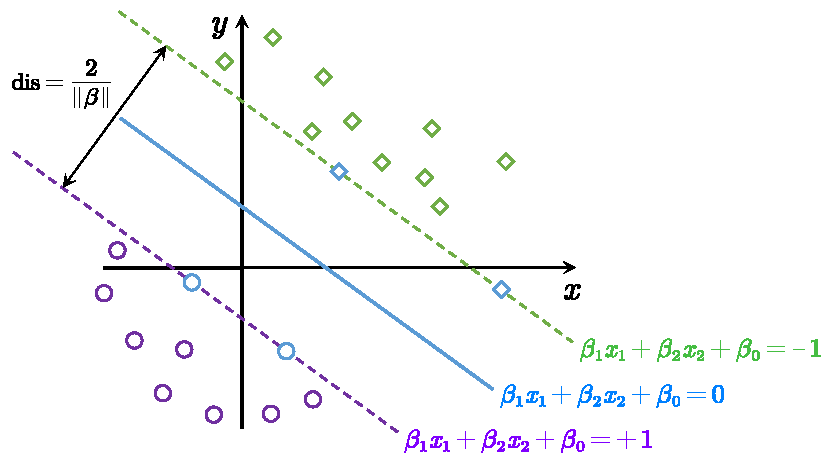
\includegraphics[width=1.0\linewidth]{SVM示意图.pdf}
			\caption{SVM示意图}
			\label{fig:svmpicture}
		\end{minipage}
		%\qquad
		\begin{minipage}{0.48\linewidth}
			\centering
			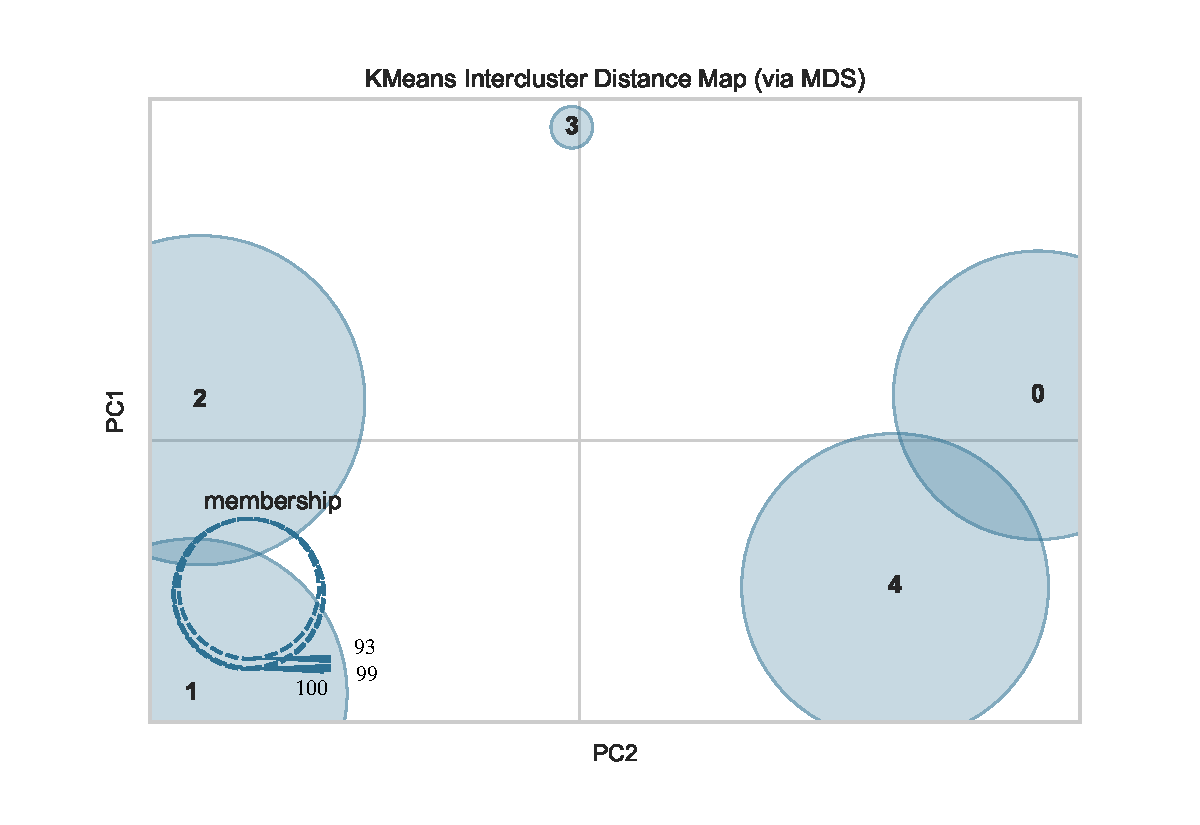
\includegraphics[width=0.85\linewidth]{类间距离.pdf}
			\caption{K-means聚类类间距离}
			\label{fig:类间距离}
		\end{minipage}
	\end{figure}

	而由于SVM多应用于解决二分类问题,且我们需要建立多分类模型,因此需要对其进行相应的改进。本文采用\textbf{OVR(One Versus Rest)}方法,将该问题改进为多个二分类问题\textcolor{blue}{\cite{psvm}}。在模型的训练时,任意将某一类别记为一类,其余类别记为另一类别,依次下去,建立出多分类的SVM模型。而对于核函数的选择,本文选择高斯核函数进行求解,其定义公式如下
	\begin{equation}
		K\left(x_i, x_j\right)=\exp \left(-\frac{\left\|x_i-x_j\right\|^{2}}{2\sigma^{2}}\right)=\exp \left(-\gamma \left\|x_i-x_j\right\|^{2}\right) \label{fgauss}
	\end{equation}
	对于高斯核函数,其可以反映出样本两点之间的相似度大小。当$\sigma$确定后,若两点之间距离越小,则相似度趋近于1;若距离越大,则相似度趋近于0。

	根据上述分析,我们利用Python的sklearn第三方库\textcolor{blue}{\footnote{sklearn第三方库具有各种分类,回归和聚类算法,包括支持向量机,随机森林,梯度提升,K均值与DBSCAN等,并且旨在与Python数值科学库NumPy和SciPy联合使用。}}建立SVM算法模型,对单词分类进行学习、预测,划分训练集及测试集比例为$8:2$,最终得到预测单词难度的分类模型,通过计算,其准确率高达$95\,\%$。本文将在后续对上述单词聚类、难度分类模型进行综合分析,讨论模型效果。

	\subsubsection{单词属性与难度之间关联分析}
	本部分我们将依据上述建立的单词聚类、难度分类模型的结果,对单词属性与难度之间的关联进行分析,首先我们为了得到单词各属性对难度的影响,我们绘制PCA双标图及21项列数据对于单词难度分类的皮尔逊相关系数热力图,如\textcolor{blue}{\cref{fig:PCA双标图}}及\textcolor{blue}{\cref{fig:21项列数据对单词难度分类皮尔逊相关系数}}所示。

	\begin{figure}[H]
		\centering
		\begin{minipage}{0.48\linewidth}
			\centering
			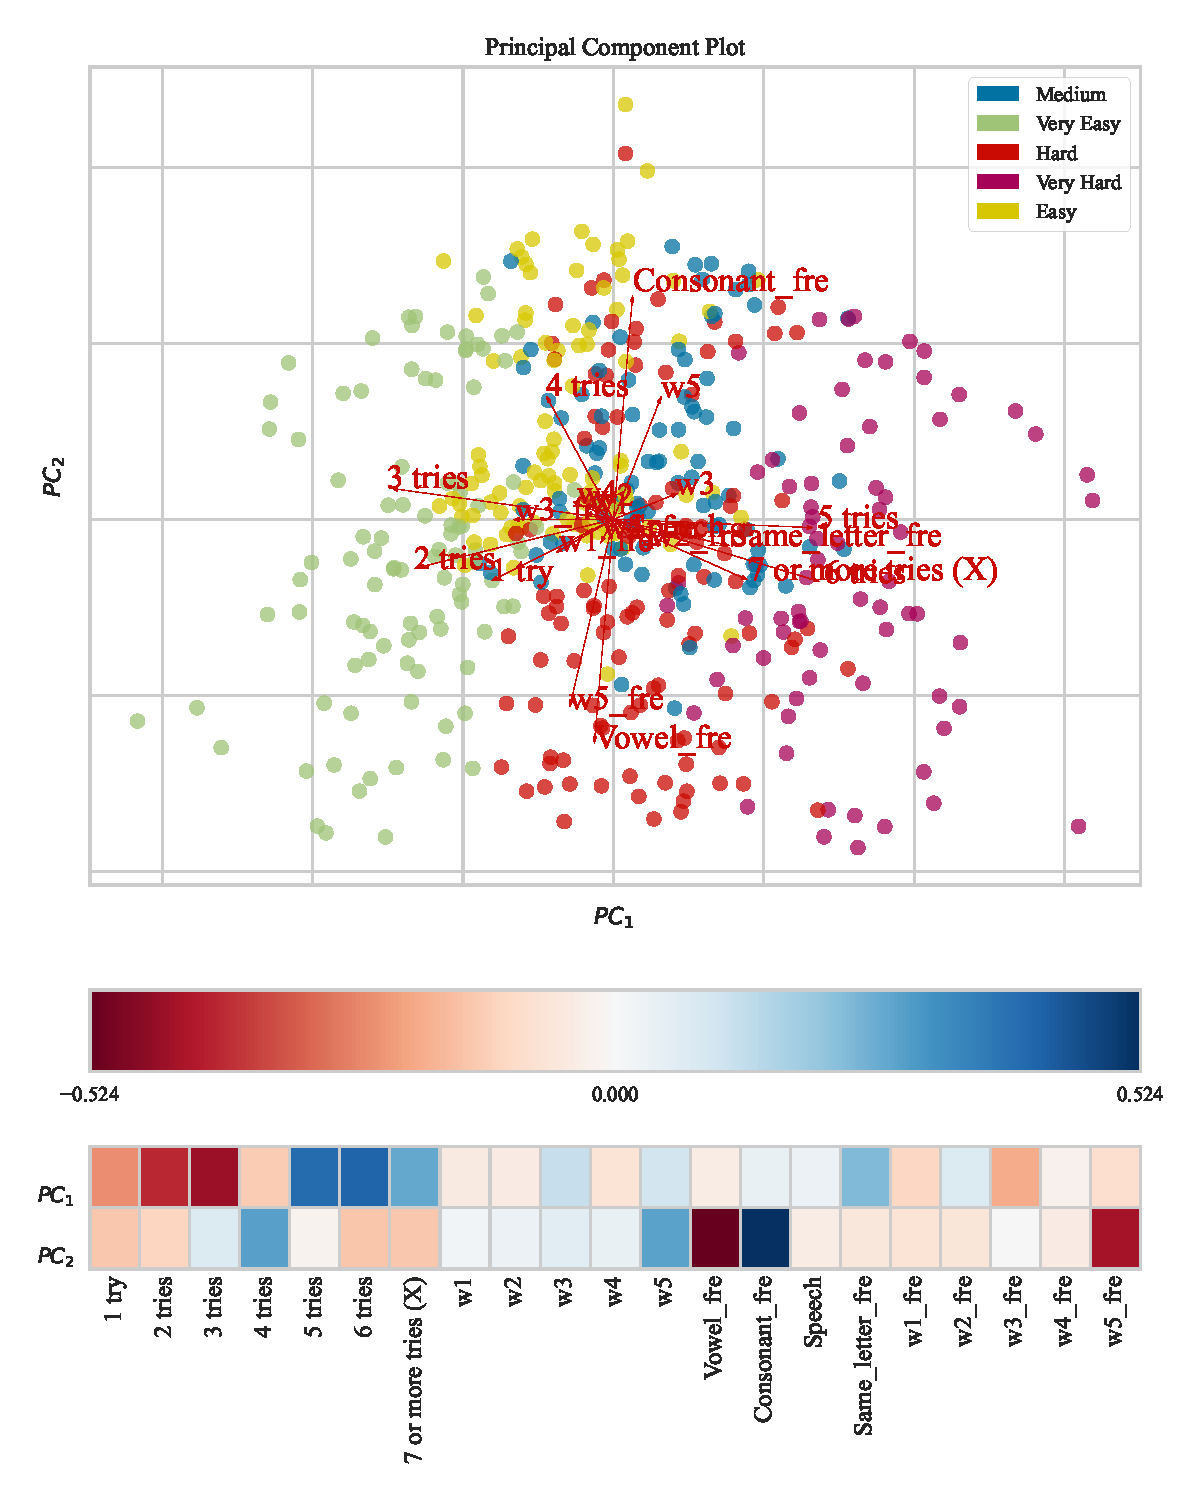
\includegraphics[width=0.90\linewidth]{PCA-2.pdf}
			\caption{主成分分析PCA双标图}
			\label{fig:PCA双标图}
		\end{minipage}
		%\qquad
		\begin{minipage}{0.48\linewidth}
			\centering
			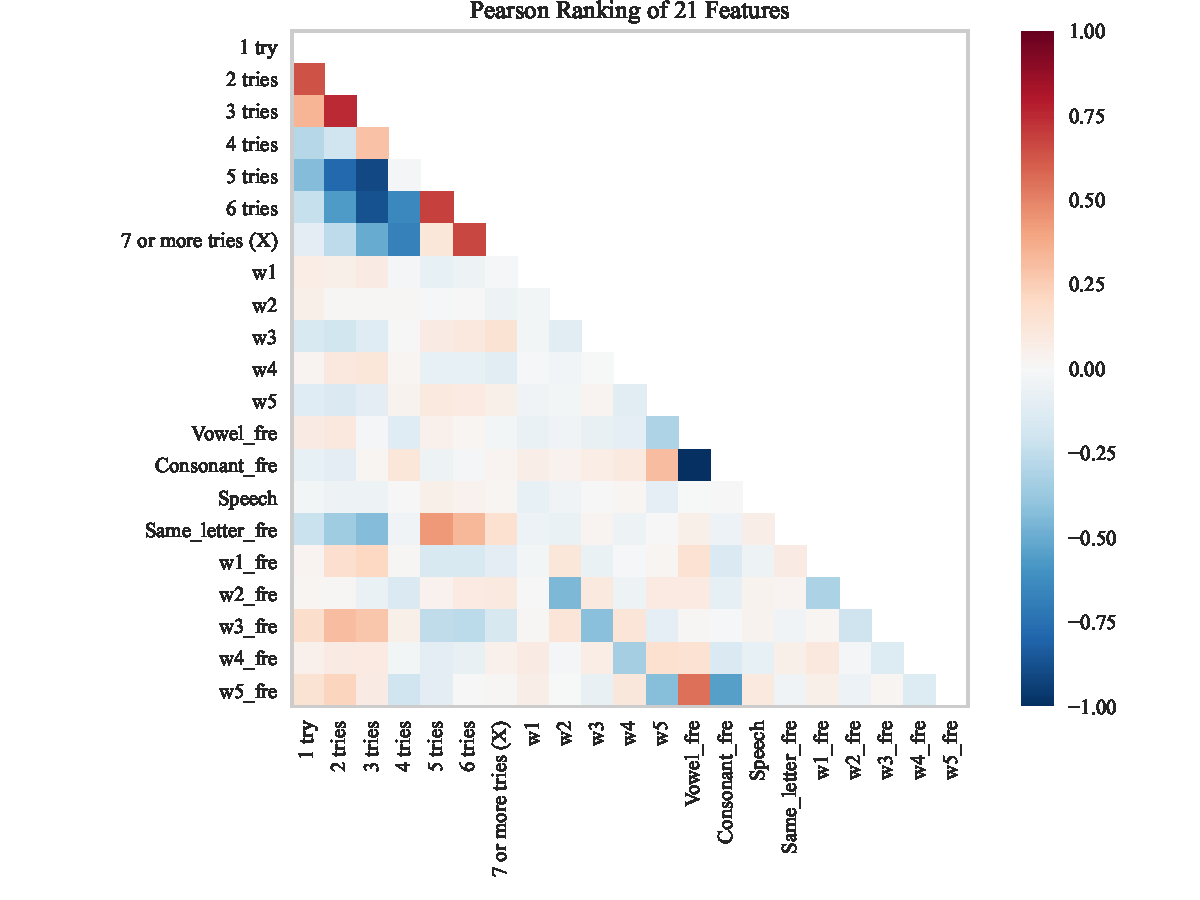
\includegraphics[width=0.95\linewidth]{Rank2D.pdf}
			\caption{与单词难度有关列数据皮尔逊相关系数}
			\label{fig:21项列数据对单词难度分类皮尔逊相关系数}
		\end{minipage}
	\end{figure}

	分析上述两幅图,我们可以发现,对于主成分PC1,我们可以发现其与“5 tries”“6 tries”“7 or more tries (X)”“Same\_letter\_fre”呈高度的正相关性,与“w3”“w5”“Consonant\_fre”“Speech”“w2\_fre”呈一般正相关性;同时其与“1 try”“2 tries”“3 tries”“w3\_fre”呈高度的负相关性,与“4 tries”“w1”“w2”“w4”“Vowel\_fre”“w1\_fre”\\“w5\_fre”呈一般负相关。对应于双标图,我们可以发现,当PC1越大时,即与其呈正相关的指标表现越明显(或与其呈负相关的指标表现越差)时,所猜词汇难度也就越大,反之,所猜词汇难度也就越低。对于主成分PC2,我们可以发现其与“Consonant\_fre”“4 tries”“w5”呈高度的正相关性,与“3 tries”“w1”“w2”“w3”“w4”“w5”呈若相关性,与“w\_5”“Vowel”呈高度的负相关性,对应于双标图,我们可以发现,当PC2发生变化时,影响所猜测词汇在难度上的变化不大,但容易区分出困难与中等难度的单词。同时我们可以发现对于主成分PC1可以区分词汇属于非常容易、非常困难,而对于主成分PC2,可以区分词汇属于困难、容易、中等难度。而对于组成上述二维主成分,可以在\textcolor{blue}{\cref{fig:PCA双标图}}中查看,同时可观察\textcolor{blue}{\cref{fig:21项列数据对单词难度分类皮尔逊相关系数}}得出相应结论。

	此外我们还绘制Shapiro特征重要性排序及特征划分难度RadViz图示,如\textcolor{blue}{\cref{fig:Shapiro}}\\
	及\textcolor{blue}{\cref{fig:RadViz}}所示。根据图中信息我们可以发现,字母在日常中出现的频率、信息熵、流行度对单词难度的影响较大,而词性与是否为元音相对于其他因素而言对难度的影响较小。玩家尝试的次数越多,该单词的难度越大,单词中的字母若在日常出现的频率较低,玩家猜出单词的可能性小,该词的难度较大,同时该单词若是当今人人了解的,流行度高热词,玩家猜对的可能性大,单词的难度较小。可以发现一个词中重复单词数对玩家尝试次数影响较大,尝试次数变多说明词的难度较大,玩家很难以较少的次数猜对。
	\begin{figure}[htbp]
		\centering
		\begin{minipage}{0.48\linewidth}
			\centering
			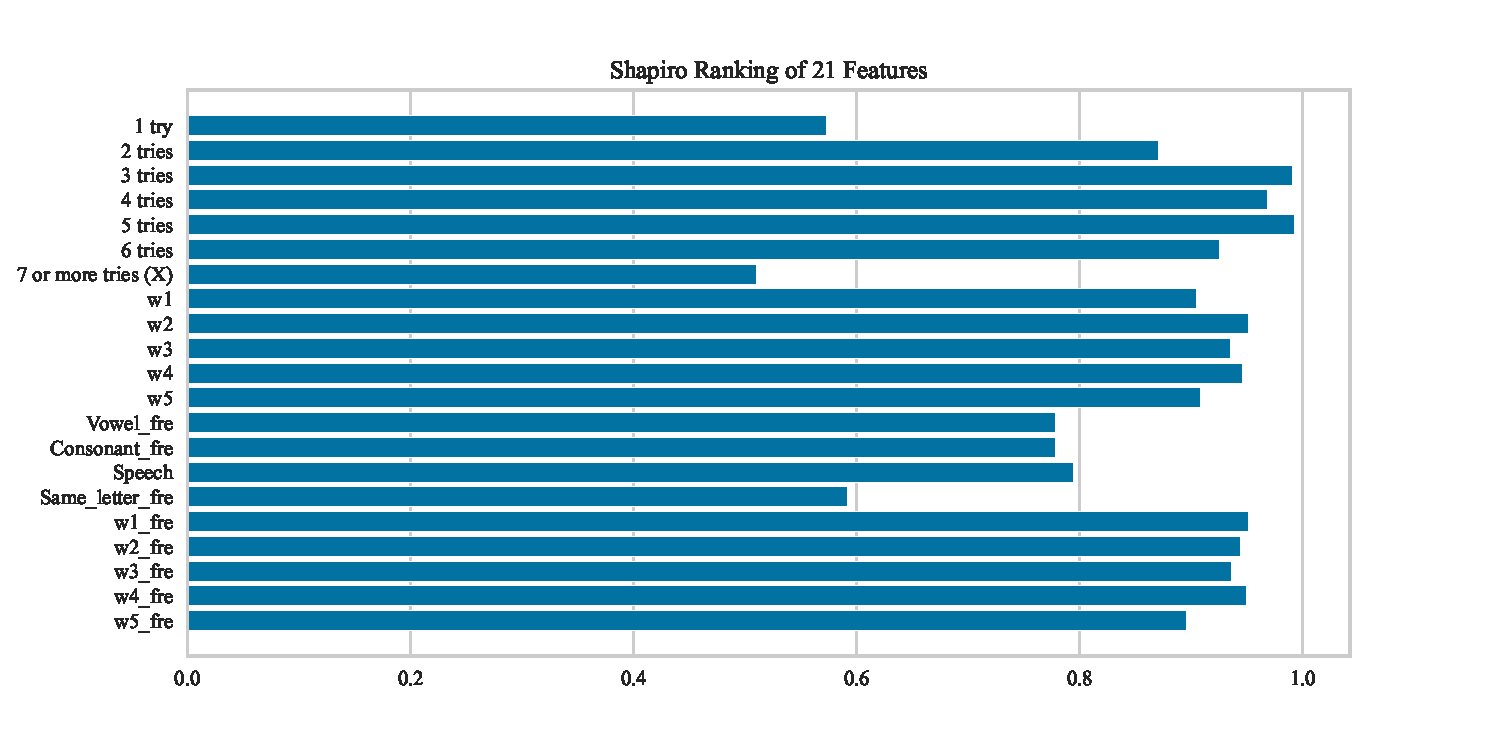
\includegraphics[width=0.90\linewidth]{Rank1D.pdf}
			\caption{Shapiro特征重要性排序}
			\label{fig:Shapiro}
		\end{minipage}
		%\qquad
		\begin{minipage}{0.48\linewidth}
			\centering
			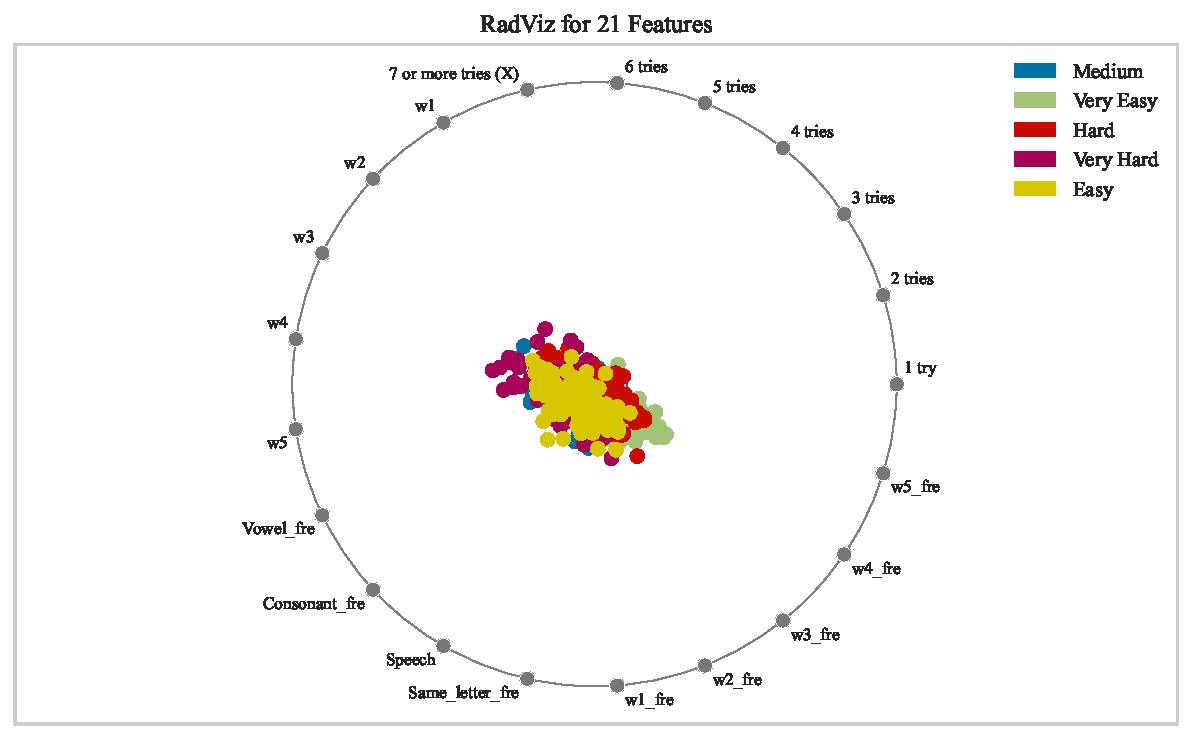
\includegraphics[width=0.82\linewidth]{RadViz.pdf}
			\caption{特征划分难度RadViz}
			\label{fig:RadViz}
		\end{minipage}
	\end{figure}

	\subsubsection{预测单词“EERIE”难度}
	这里我们利用上述建立的单词聚类、难度分类,即基于K-means及SVM模型,我们可以对给定单词“EERIE”进行难度的分类预测,最终模型结果将其划分为$2$类,对应于\textcolor{blue}{\cref{tab:类别与难度的对应关系}},我们可以得到单词“EERIE”的难度为“困难(Hard)”。同时对于SVM多分类,我们有$94.74\,\%$的把握认为本文对于单词难度的划分分类预测结果正确。
	
	\subsubsection{模型效果分析}
	为了评估我们建立模型效果,我们针对K-means聚类及SVM多分类分别进行详细分析。
	
	对于K-means聚类,我们计算其\textbf{聚类轮廓系数(Silhouette Coefficient,SC)}。轮廓系数结合了聚类的\textbf{凝聚度(Cohesion)}与\textbf{分离度(Separation)},用于评估聚类效果。该值处于$\left[-1,1\right]$之间,值越大,则代表聚类效果越好。对于样本点$i$其轮廓系数为
	\begin{equation}
		\text{SC}\left(i\right)=\frac{b\left(i\right)-a\left(i\right)}{\max\left\{a\left(i\right),b\left(i\right)\right\}}
	\end{equation}
	其中$a\left(i\right)$为对于每一样本点$i$,与其同一类中其他样本点的平均距离,$b\left(i\right)$为样本点$i$与其他类中样本点的平均距离。
	
	对于整个聚类,其轮廓系数为所有样本点轮廓系数的均值。因此,首先我们绘制出K-means聚类的各类别轮廓系数可视化,如\textcolor{blue}{\cref{fig:轮廓系数}}所示。并计算出聚类综合轮廓系数(即均值)为$0.1225$,通过查阅相关资料\textcolor{blue}{\cite{k-means}},可以认为该平均聚类轮廓系数达到聚类效果较好的水平。

	同时我们还绘制K-means模型类间距离可视化,如\textcolor{blue}{\cref{fig:类间距离}}所示。类间距离显示了某类中心在二维空间的投影,并保留了到其他中心的距离。可视化中的中心越接近,它们在原始特征空间中的距离就越近。集群的大小是根据评分指标确定的。默认情况下,它们是按成员资格大小的,例如,属于每个中心的实例数量\textcolor{blue}{\cite{类间距离}}。然而,由于类别在2D投影,因此可能在可视化中发现类与类之间存在重叠现象,但这并不意味着它们在原始特征空间中重叠,即在高维度内,他们聚类效果明显且效果优秀。

	对于SVM多分类预测模型,其预测准确率在测试集上可达到$94.74\,\%$,预测精度较高,效果较优秀。
	\subsection{问题四}\label{问题四}
	对于该问题,我们需要更深次地挖掘数据,发现更多有趣的信息及结论。因此在这里我们从多方面进行分析。
	\subsubsection{每日选择困难模式人数占比变化}
	尽管随着时间的推移,Wordle游戏游玩人数已逐渐趋向于稳定,但参与困难模式的玩家数量却稳步增加。\textcolor{blue}{\cref{fig:选择困难模式游戏玩家占比变化}}是参与困难模式的玩家人数与总玩家的百分比及日变化情况,\textcolor{blue}{\cref{fig:选择困难模式游戏玩家占比变化回归}}为每日选择困难模式人数占比线性回归残差图。

	\begin{figure}[H]
		\centering
		\begin{minipage}{0.48\linewidth}
			\centering
			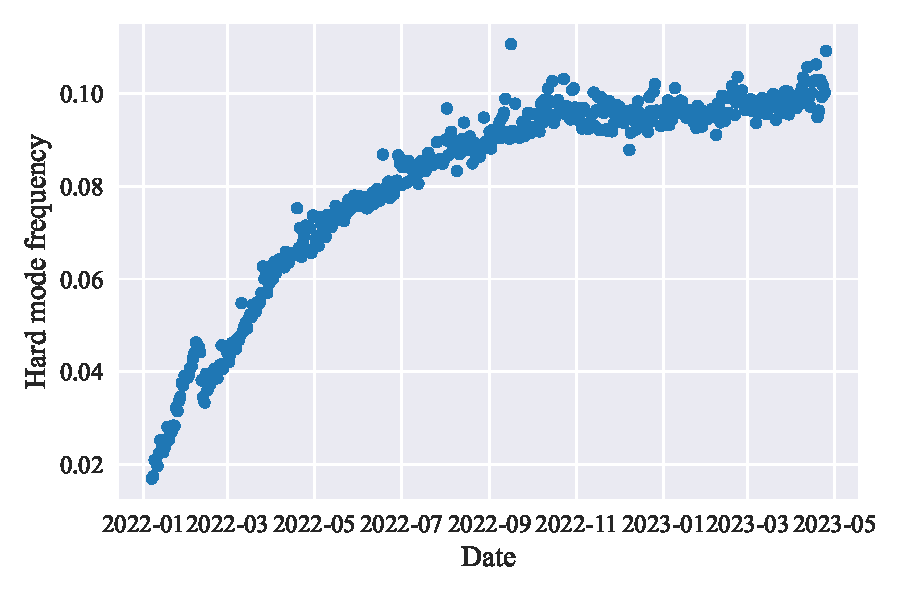
\includegraphics[width=0.98\linewidth]{选择困难游戏模式游戏的人数比例.pdf}
			\caption{选择困难模式游戏玩家占比变化情况}
			\label{fig:选择困难模式游戏玩家占比变化}
		\end{minipage}
		%\qquad
		\begin{minipage}{0.48\linewidth}
			\centering
			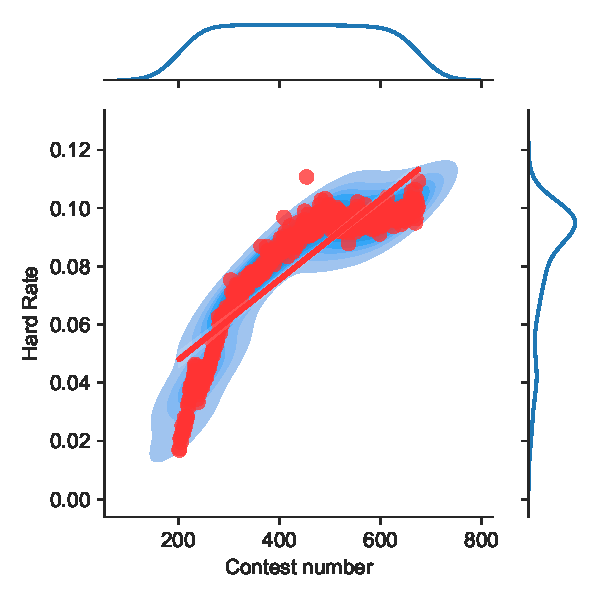
\includegraphics[width=0.66\linewidth]{选择困难游戏模式游戏的人数比例核密度.pdf}
			\caption{选择困难模式游戏玩家占比变化回归}
			\label{fig:选择困难模式游戏玩家占比变化回归}
		\end{minipage}
	\end{figure}

	\subsubsection{谜题难度}
	我们发现对于谜题难度,五类难度的单词呈周期性出现,即当天难度与前一天或后一天均有可能不同,但在整体上呈现出周期性变化。同时,我们还发现不同难度的词汇作为谜题,出现的频率大致相同。但为了让更多玩家能够挑战成功,标记为非常困难(Very Hard)的单词出现频率较低。

	\begin{figure}[H]
		\centering
		\begin{minipage}{0.48\linewidth}
			\centering
			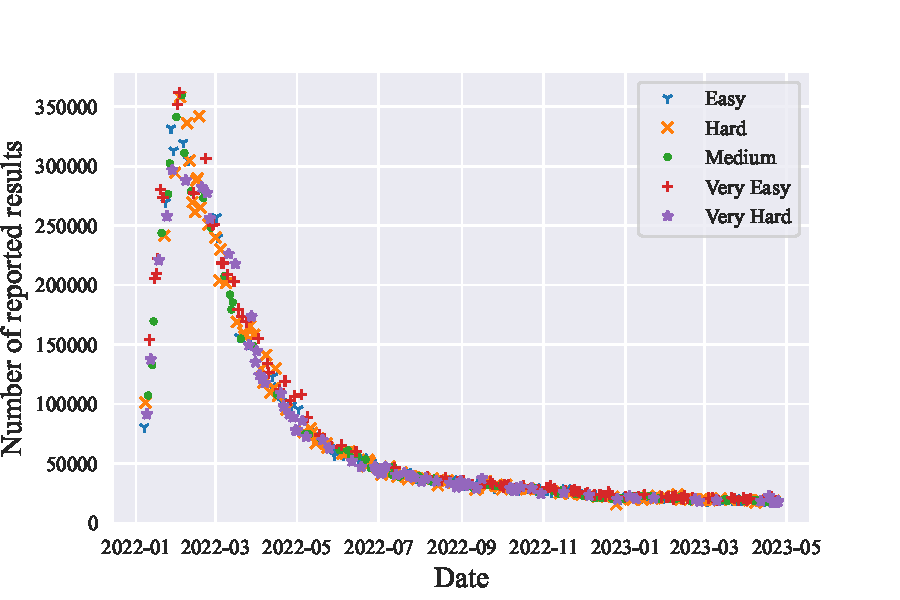
\includegraphics[width=0.98\linewidth]{WordleClass.pdf}
			\caption{Wordle词汇每日难度变化情况}
			\label{fig:WordleClass}
		\end{minipage}
		%\qquad
		\begin{minipage}{0.48\linewidth}
			\centering
			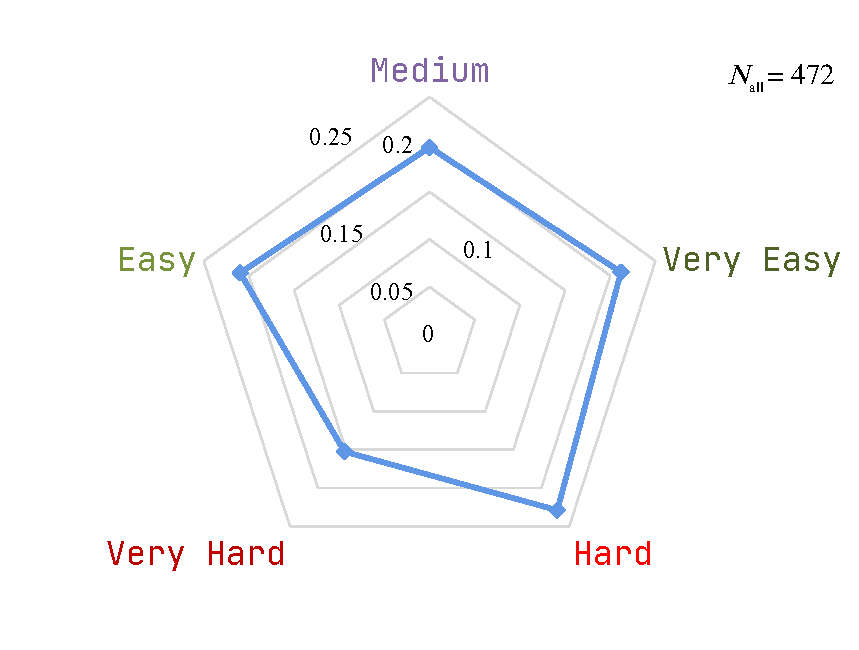
\includegraphics[width=0.95\linewidth]{不同难度单词频率.pdf}
			\caption{不同难度单词出现频率}
			\label{fig:不同难度单词频率}
		\end{minipage}
	\end{figure}

	\subsubsection{玩家尝试次数百分比}
	尽管每日玩家猜测单词次数百分比有一定变化,但从时间序列整体上看,其在一定范围内稳定。同时我们还计算了从2022年1月7日至2023年4月25日共计472条竞赛数据\textcolor{blue}{\footnote{实际上应该有474条数据,但由于官方在2023年1月31日及2023年2月17日因某些原因并未统计出当日当日数据。}}(这里的时间对应于美国西五区时间)每日玩家尝试次数百分比均值,发现其在整体上符合正态分布。

	\begin{figure}[H]
		\centering
		\begin{minipage}{0.48\linewidth}
			\centering
			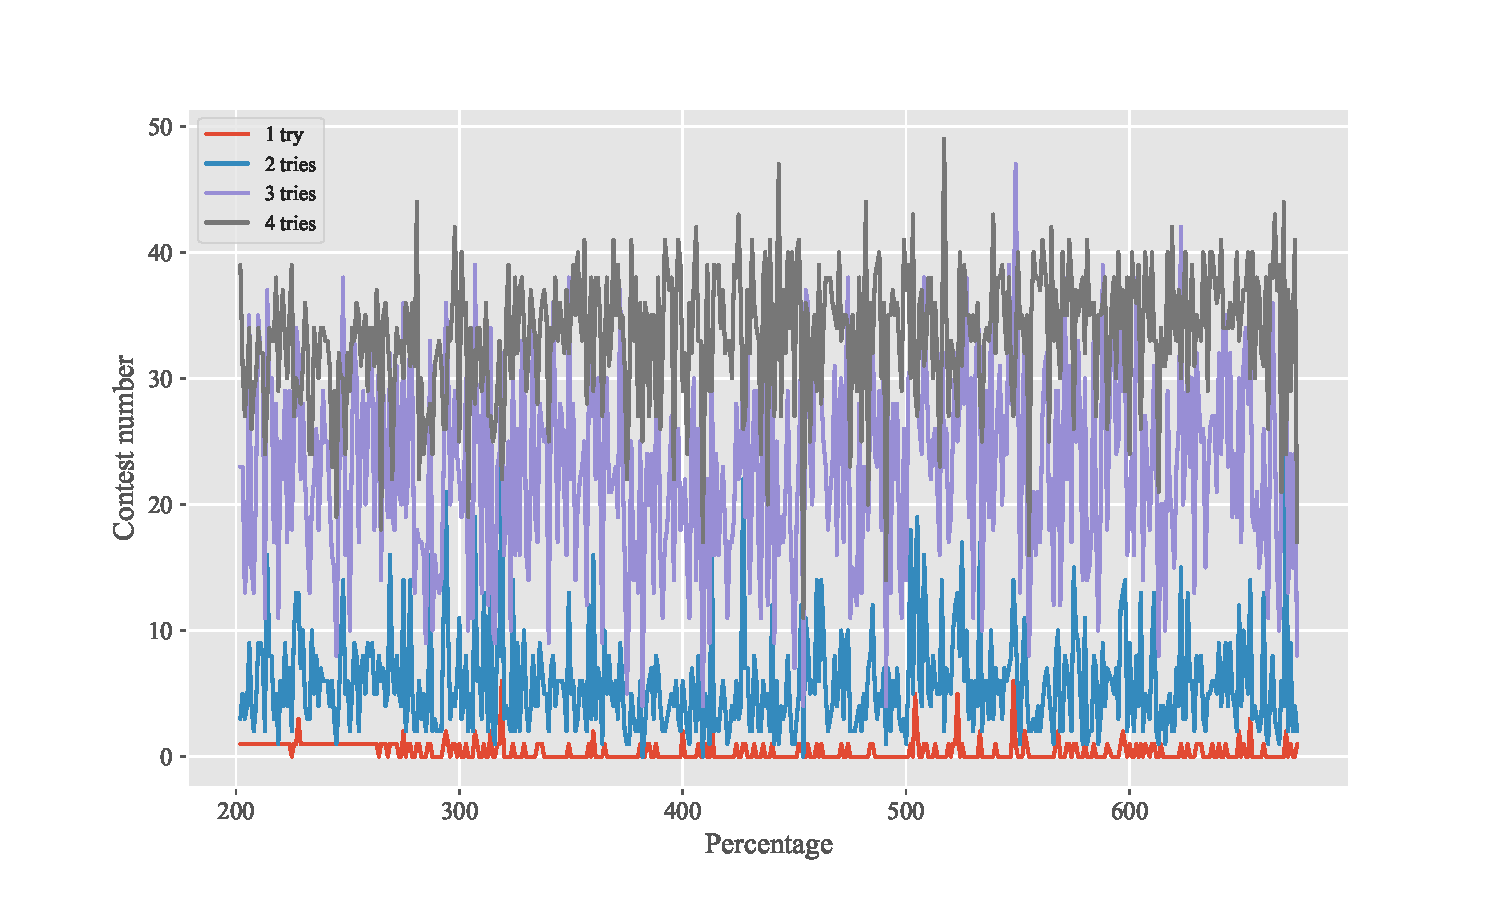
\includegraphics[width=1.0\linewidth]{尝试次数分布1.pdf}
			\caption{玩家尝试次数(1,2,3,4)每日变化}
			\label{fig:尝试次数分布1}
		\end{minipage}
		%\qquad
		\begin{minipage}{0.48\linewidth}
			\centering
			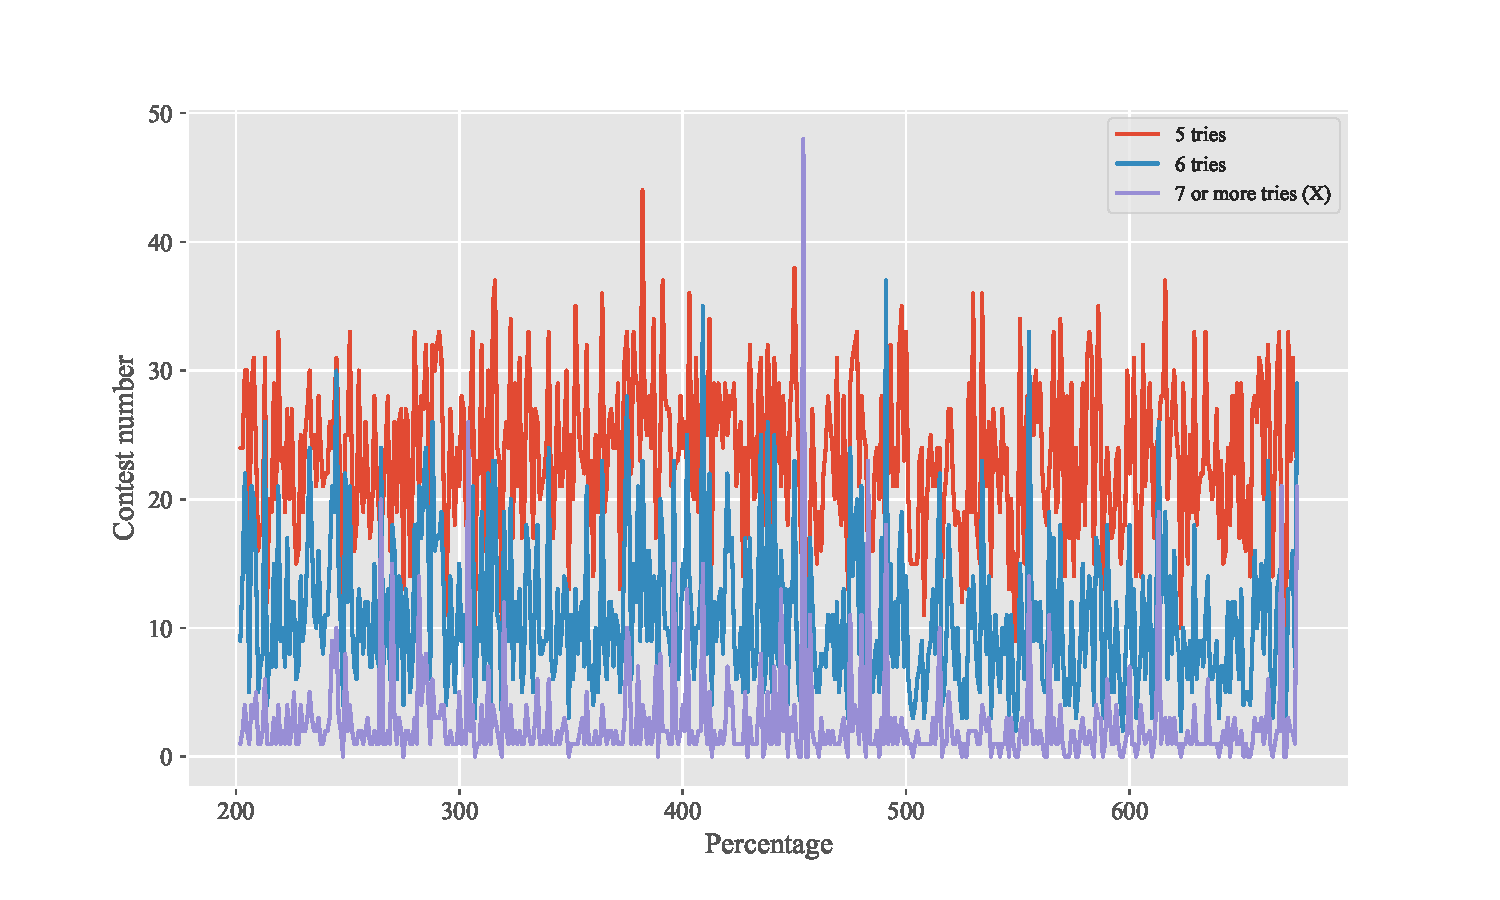
\includegraphics[width=1.0\linewidth]{尝试次数分布2.pdf}
			\caption{玩家尝试次数(5,6,X)每日变化}
			\label{fig:尝试次数分布2}
		\end{minipage}
	\end{figure}

	这里我们分析游戏编号为$483$,即2022年10月15日的数据,我们可以发现对于尝试7次及以上玩家占整体玩家的$23\,\%$,对应的单词为“CATCH”,在先前分析中,我们定义其难度为非常困难(Very Hard),结合先前分析,我们可以发现对于该单词,其由$1$个元音字母构成,重复字母数为$2$个,且其各位字母在常用英文词中出现频率较低,符合先前分析。

	\begin{figure}[H]
		\centering
		\begin{minipage}{0.48\linewidth}
			\centering
			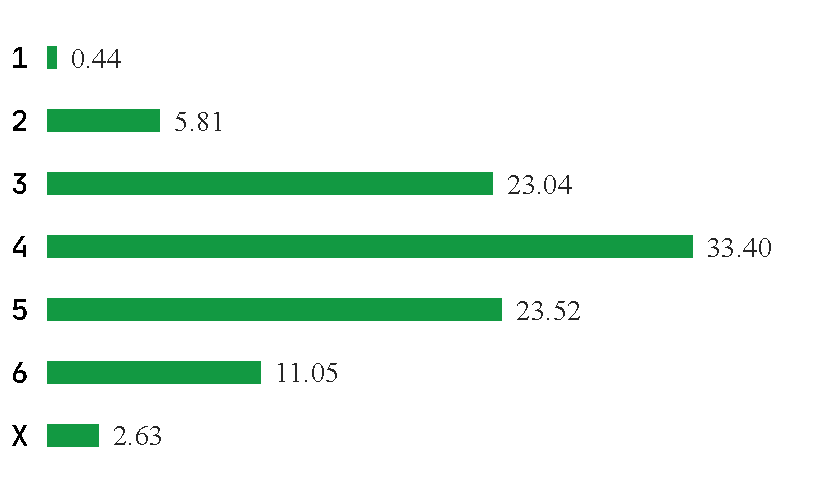
\includegraphics[width=1.0\linewidth]{尝试次数分布总.pdf}
			\caption{游戏玩家平均尝试次数分布}
			\label{fig:尝试次数分布总}
		\end{minipage}
		%\qquad
		\begin{minipage}{0.48\linewidth}
			\centering
			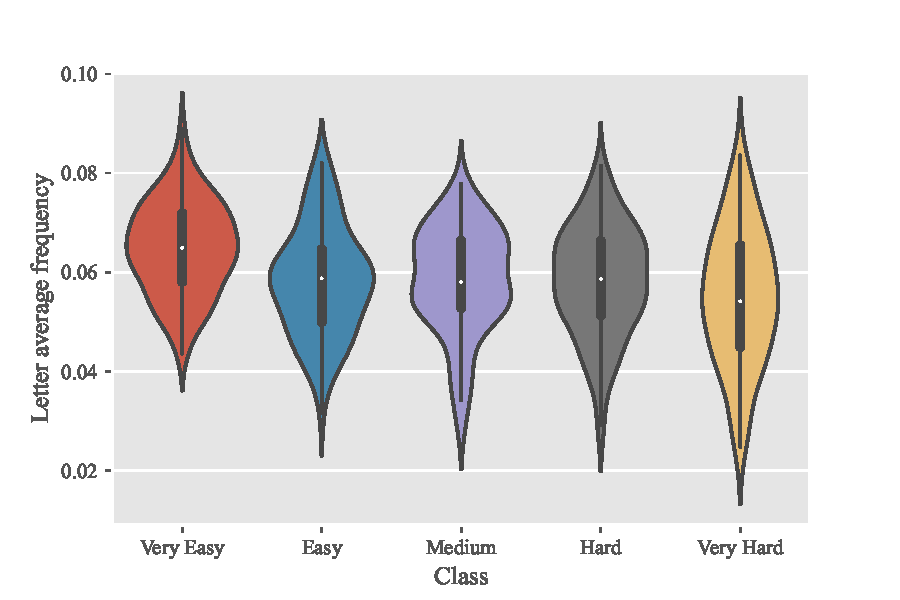
\includegraphics[width=0.8\linewidth]{单词字母平均出现率与难度.pdf}
			\caption{单词字母平均出现率与单词难度}
			\label{fig:单词字母平均出现率与单词难度}
		\end{minipage}
	\end{figure}

	\subsubsection{小提琴图数据特征分析}
	我们发现,对于某一单词而言,其各位上字母在常用英文单词中出现的概率越高,该词越有可能被划分为容易类别,反之,越不容易被划分为容易类别。但是,对于某些单词而言,若其每位字母出现频率均值较高也有可能被划分为困难类别,这可能是由于单词其他属性对其产生影响,如\textcolor{blue}{\cref{fig:单词字母平均出现率与单词难度}}所示。

	我们发现选择困难模式的占比与单词的难易程度基本没有关系,而单词的某些词性却影响着困难模式的占比,如VB、IN、VBZ等。在这些词性中,困难模式的占比较为平均,没有出现主要集中在某一比例的现象,如\textcolor{blue}{\cref{fig:困难模式占比与难度}}及\textcolor{blue}{\cref{fig:困难模式占比与词性}}所示。

	对于影响平均尝试次数的因素,不同的单词难度对次数的影响尤为明显,随着难度上升,玩家尝试的次数也随之增加。同时单词词性也将在一定程度上影响着玩家平均尝试的次数,如当日单词词性为NN、RB、NN等,玩家整体在尝试次数上分布差异较大,如\textcolor{blue}{\cref{fig:平均尝试次数与难度}}及\textcolor{blue}{\cref{fig:平均尝试次数与词性}}所示。

	\begin{figure}[H]
		\centering
		\begin{minipage}{0.48\linewidth}
			\centering
			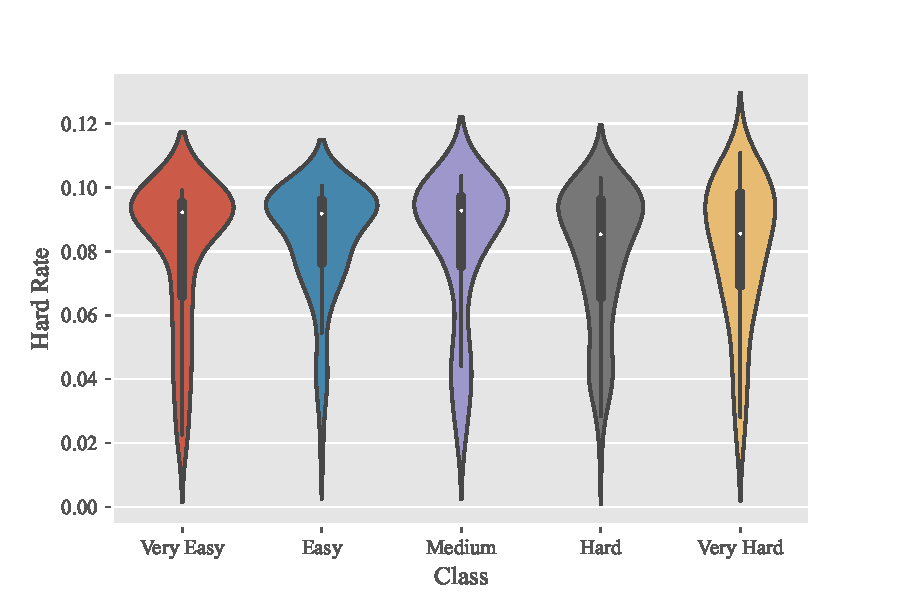
\includegraphics[width=0.95\linewidth]{选择困难模式占比与难度.pdf}
			\caption{困难模式占比与难度}
			\label{fig:困难模式占比与难度}
		\end{minipage}
		%\qquad
		\begin{minipage}{0.48\linewidth}
			\centering
			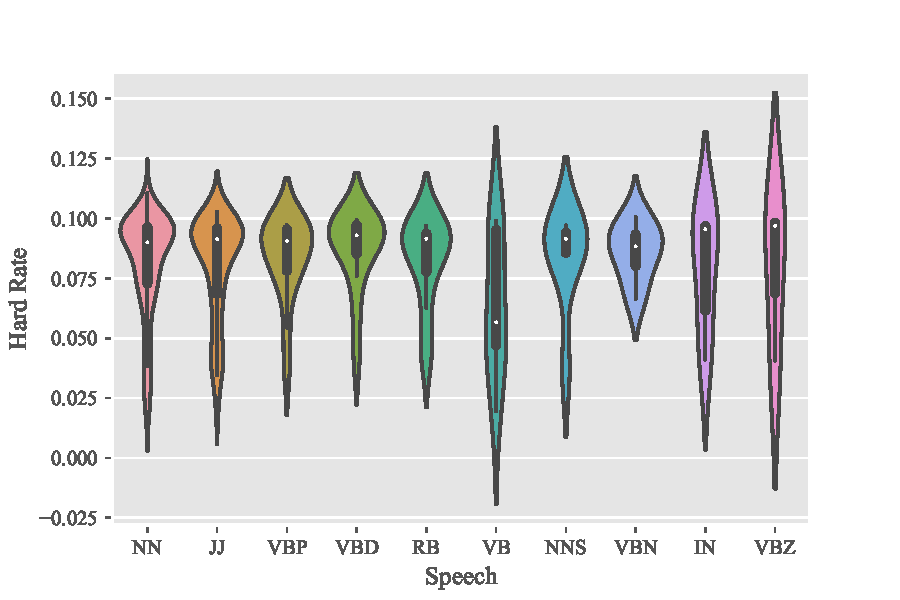
\includegraphics[width=0.95\linewidth]{选择困难模式占比与词性.pdf}
			\caption{困难模式占比与词性}
			\label{fig:困难模式占比与词性}
		\end{minipage}
	\end{figure}

	\begin{figure}[H]
		\centering
		\begin{minipage}{0.48\linewidth}
			\centering
			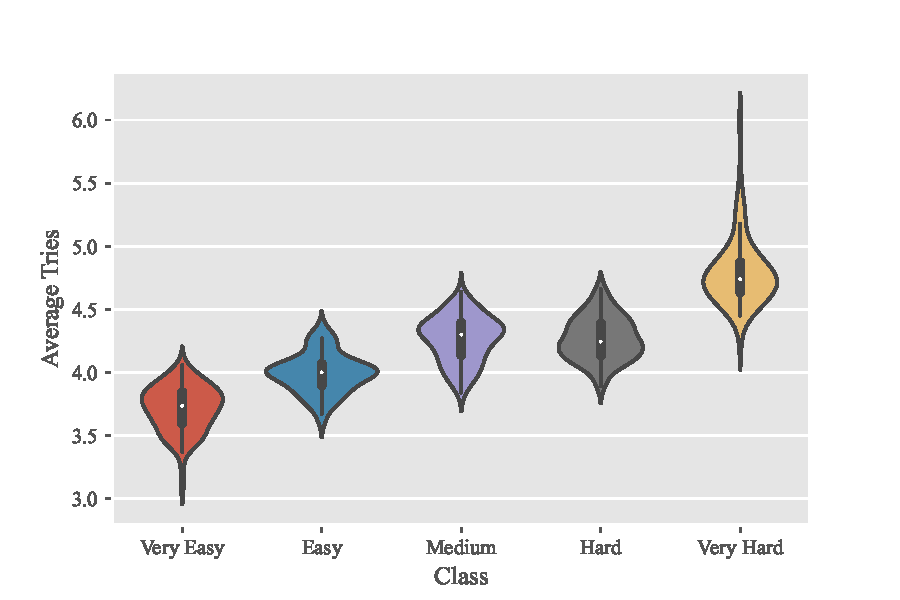
\includegraphics[width=0.95\linewidth]{平均尝试次数与难度.pdf}
			\caption{平均尝试次数与难度}
			\label{fig:平均尝试次数与难度}
		\end{minipage}
		%\qquad
		\begin{minipage}{0.48\linewidth}
			\centering
			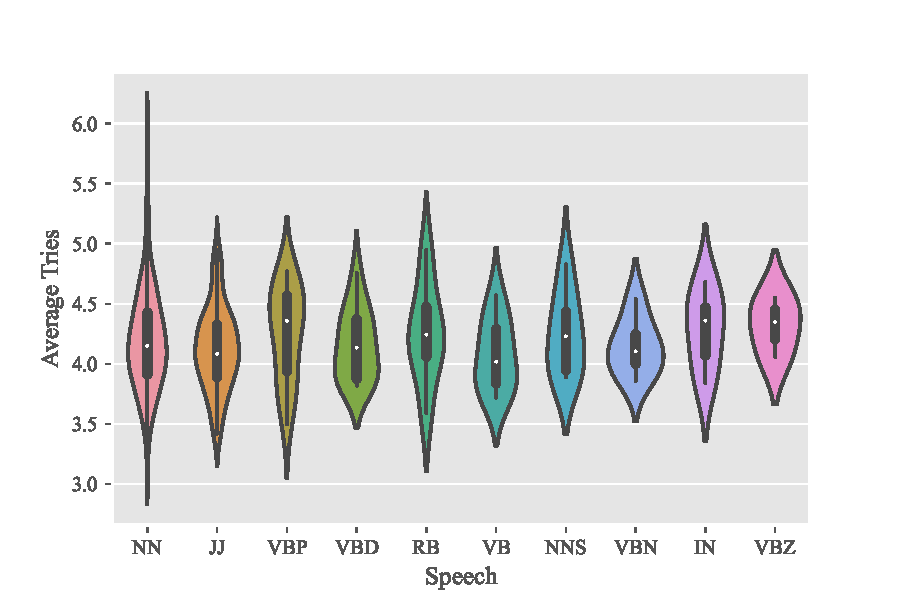
\includegraphics[width=0.95\linewidth]{平均尝试次数与词性.pdf}
			\caption{平均尝试次数与词性}
			\label{fig:平均尝试次数与词性}
		\end{minipage}
	\end{figure}

	当单词中相同字母的个数增加时,玩家尝试次数先增加后减少,过多和过少的重复字母都会使玩家快速得到正确答案。而单词的不同元音个数和词性对玩家尝试次数影响大较小。

	\begin{figure}[H]
		\centering
		\begin{minipage}{0.48\linewidth}
			\centering
			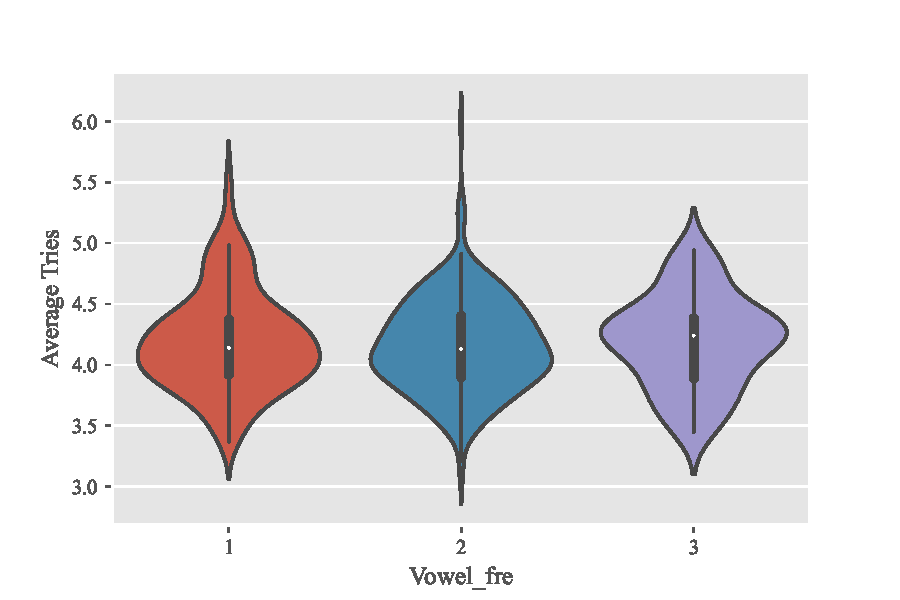
\includegraphics[width=0.95\linewidth]{平均尝试次数与单词中元音个数.pdf}
			\caption{平均尝试次数与单词中元音字母个数}
			\label{fig:平均尝试次数与单词中元音字母个数}
		\end{minipage}
		%\qquad
		\begin{minipage}{0.48\linewidth}
			\centering
			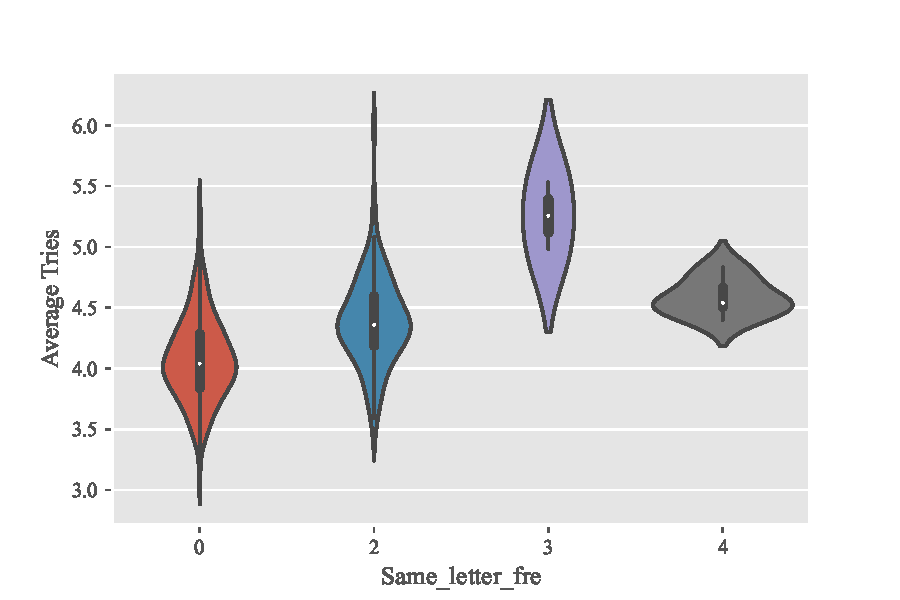
\includegraphics[width=0.95\linewidth]{平均尝试次数与单词中相同字母个数.pdf}
			\caption{平均尝试次数与单词中相同字母个数}
			\label{fig:平均尝试次数与单词中相同字母个数}
		\end{minipage}
	\end{figure}

	\subsection{问题五}
	对于该问题,我们需要总结问题一至四分析结果,并向纽约时报的谜题编辑总结本文结果并提出相关建议。这里我们书写英文及中文各一份,方便读者阅读。
	\newpage
	\centerline{{\Large \textbf{Wordle Game Explored}}}\label{问题五}
	~\\
	\noindent \textbf{To}: Puzzle Editor, The New York Times\\
	\noindent \textbf{From}: Wordle game fans\\
	\noindent \textbf{Date}: May 2, 2023\\
	\noindent \textbf{Subject}: Some research and suggestions about Wordle\\
	\noindent\rule{\textwidth}{1.2pt}
	\textbf{Dear New York Times Wordle puzzle editor:}

	Hello! We are a team of three Wordle enthusiasts. In order to make the game have more room for development, attract more players and increase its value, we have studied the pattern of difficulty change of the game and the chain reaction caused by the difficulty change. This letter is written to share with you the results of our analysis and research.

	We found that for game propagation, it generally goes through periods of growth, maturity, decline and stability. Through our analysis, we found that the total number of players gradually tends to be stable from June 2022, which also means that the player base has been basically fixed. At the same time, we also conducted relevant statistics and found that the total number of words with 5 characters exceeds 12,000, and if we do not include excessively rare words, the range of game answers can still reach about 2,500 words, and such a vocabulary base can last for nearly 7 years. Therefore, we studied the data reported from January 7, 2022 to April 25, 2023 to build a comprehensive model of regression, clustering, and classification prediction to explore the Wordle game. For example, we found a correlation between word attributes and difficulty mode scores, and we found that too many or too few repetitive letters in a word can affect the player's score situation. In addition, when the puzzle words contain fewer letters involved in common English words, their difficulty will be higher. Accordingly, the proportion of unsuccessful answers and successes after 4$\sim$6 attempts on the same day will also increase significantly.

	Based on these findings, we give the following recommendations for the operation of the game:

	\begin{itemize}
		\item \textbf{Update the word bank and optimize word selection. }
		
		We found that a relative portion of the currently completed daily challenges do not conform to the normal distribution of attempts, i.e., excessively difficult or excessively easy. To solve this problem, we have created a comprehensive analysis model of word clustering and difficulty classification, according to which you can easily eliminate unsuitable words and select new suitable words to form a new word bank. This can return the game to its own entertainment nature, so that more people are willing to participate in it.

		\item \textbf{Update the mode and set the ranking. }
		
		We found that the current mode of play is rather monotonous, so the number of players per day is decreasing to some extent. We propose to add a leveling mode and a matchmaking mode. Breakthrough mode: from easy to hard, we can set the very easy part of words filtered in the first suggestion as the starting level of the breakthrough mode, and then from easy to hard; Battle mode: players will be randomly matched with players to battle against each other 5 words to be the first to answer 3 as the winner. This scheme can increase the fun of the game and attract old players to return to the game and new players to join the game. We also suggest applying to users for access to their social media, reading the scores of their friends participating in the game and setting up a leaderboard. This solution can increase the game's player participation, enhance its social interaction, and get more and more people involved.

		\item \textbf{Lowering the threshold and providing assistance. }
		
		With the popularity of the Internet, in order to let more people participate, we suggest classifying the game in primary, intermediate and advanced modes, where the primary and intermediate levels provide hint functions, 4 times and 2 times respectively. The advanced mode no longer provides hints. This solution will allow English beginners to learn better, in other words, "teaching for fun", and enhance the educational aspect of the game, while allowing players of different English levels to have a high level of participation.

		\item \textbf{Actively promote and increase the number of languages. }
		
		As an international game, while optimizing the game, we should also focus on the promotion of the game to ensure more new players come in. At the same time, although Wordle is currently updated with multiple languages, there are still gaps in smaller languages, and we suggest further increasing support for other languages to allow more people around the world to participate.
	\end{itemize}

	Thank you for reading our letter in your busy schedule! At the same time, we sincerely hope that our suggestions will help Wordle to develop better and increase the value of its existence on multiple levels.

	~\\
	\noindent \textbf{Yours Sincerely,}\\
	\noindent \textbf{Wordle game fans}\\

	\newpage
	\centerline{{\Large \textbf{Wordle游戏的探讨}}}
	~\\
	\noindent \textbf{收件人}: 《纽约时报》Wordle谜题编辑\\
	\noindent \textbf{发件人}: Wordle游戏爱好者\\
	\noindent \textbf{日期}: 2023年5月2日\\
	\noindent \textbf{主题}: 关于Wordle游戏的一些研究与建议\\
	\noindent\rule{\textwidth}{1.2pt}
	\noindent {\heiti 尊敬的纽约时报Wordle谜题编辑:}

	{\heiti 您好!}

	我们是由三个Wordle爱好者组成的团队,为了使游戏有更大的发展空间,吸引更多的玩家,提高其价值,我们研究了该游戏的难度变化规律及难度变化引起的连锁反应。写此信是为了与你们分享我们的分析研究结果。

	我们发现对于游戏传播而言,一般会经历增长、成熟、衰退和稳定的时期,通过分析,我们发现从2022年6月开始,游戏总人数逐渐趋近于稳定,这也意味着玩家群体已经基本固定。同时我们还进行相关统计,发现5个字符的单词总数超过12000个,若不包括过分稀有词,游戏答案的范围仍然可以达到2500个词汇左右,这样的词汇库可以持续近7年。所以我们对2022年1月7日至2023年4月25日报告数据进行研究,建立回归、聚类、分类预测的综合性模型,探讨Wordle游戏。比如我们发现单词属性与困难模式得分存在着一定的关联,我们发现单词中重复的字母过多或过少均会影响玩家得分情况。此外,当谜底单词中含有常用英语单词中涉及较少的字母时,其难度也将偏高。相应地,当日未成功答题及4至6次尝试后成功的比例也将明显上升。

	基于这些发现,我们对游戏的运行给予以下建议:

	\begin{itemize}
		\item \textbf{更新词库,优化选词。}
		
		我们发现目前已完成的每日挑战中,有相一部分不符合正常的尝试分布,即过分难或过分简单。为解决这一问题,我们建立单词聚类、难度分类的综合分析模型,依据这个模型,您可轻松地剔除不适合的单词,并挑选出新的适合的单词组成新的词库。这样能够回归游戏其本身娱乐之性质,让更多的人愿意参与进来。
		\item \textbf{更新模式,设置排行。}
		
		我们发现目前的游玩模式较为单调,因此每日玩家人数在一定程度上呈减少趋势。我们建议加入闯关模式及对战模式。闯关模式:由易及难,我们可以将第一条建议中筛选的非常容易的那一部分单词设置为闯关模式的起始关卡,随后由易及难;对战模式:玩家将随机匹配玩家进行对战5个单词以率先答出3个为胜。此方案可增加游戏的趣味性,吸引老玩家重回游戏、新玩家加入游戏。我们还建议向用户申请接入其社交媒体的权限,读取其好友中参与游戏的得分情况并设置排行榜,此方案可提高游戏的玩家参与度,增强其社交互动性,让越来越多的人参与其中。
		\item \textbf{降低门槛,提供辅助。}
		
		随着互联网的普及,为了让更多的人参与进来,我们建议对游戏进行初级、中级、高级模式分类,其中初级和中级提供提示功能,分别为4次和2次。高级模式下不再提供提示。此方案可让英语初学者得以更好地学习,换言之“寓教于乐”,增强其教育性,同时让不同英语水平的玩家都可以有较高的参与度。
		\item \textbf{积极宣传,增加语种。}
		
		作为国际化的游戏,在优化游戏的同时,也应注重游戏的宣传,确保更多的新玩家涌入。同时,尽管Wordle当前已更新多国语言,但小语种仍然存在缺口,我们建议进一步增加其他语言的支持,让世界各地更多的人参与进来。
	\end{itemize}
	
	感谢您在百忙之中阅读我们的信函!同时,我们真诚地希望我们的建议能够帮助Wordle更好地发展,在多层面提高其存在的价值。

	~\\
	\rightline{{\heiti Wordle游戏爱好者}}

	\rightline{{\heiti 2023年5月2日}}


	\newpage
	\section{模型灵敏度检验}\label{灵敏度分析}
	为了更好地分析模型效果,我们绘制出SVM多分类模型的\textbf{混淆矩阵热力图}、\textbf{分类报告}、\textbf{ROC/AUC曲线}以及\textbf{分类预测结果}。
	\begin{itemize}
		\item \textbf{混淆矩阵(Confusion Matrix)热力图}。该可视化图形的每一行表示样本标签的实际类别,在本题中表示单词难度实际类别,而每一列表示样本标签的预测类别,在本题中表示单词难度划分的预测值。因此该图示的主对角线数据之和即为模型预测准确的样本数。对于多分类模型,我们可以随机指定一类为正类,而其余就为对应的负类。这里我们需要引入四项值,分别为$TP$、$FN$、$FP$、$TN$,其中T为True,F为False,这两个字母表示预测值与实际值是否相同;P为Positive,N为Negative,这两个字母表示预测出的是属于正类(阳性)还是负类(阴性)。而混淆矩阵热力图即为这些值组成,该图示可以直观地观察到预测准确与错误的情况,以及模型对于每一类别的区分程度。模型混淆矩阵热力图见\textcolor{blue}{\cref{fig:混淆矩阵热力图}}。

		\begin{figure}[H]
			\centering
			\begin{minipage}{0.48\linewidth}
				\centering
				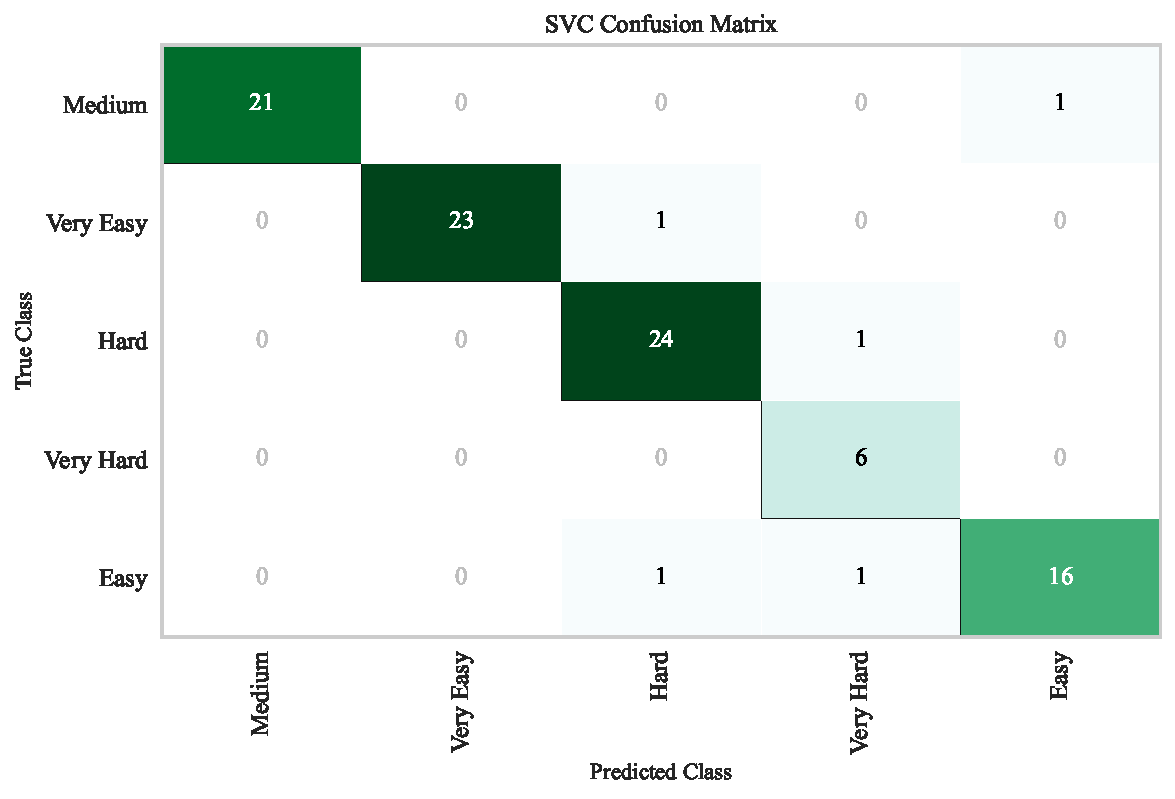
\includegraphics[width=0.90\linewidth]{混淆矩阵热力图.pdf}
				\caption{混淆矩阵热力图}
				\label{fig:混淆矩阵热力图}
			\end{minipage}
			%\qquad
			\begin{minipage}{0.48\linewidth}
				\centering
				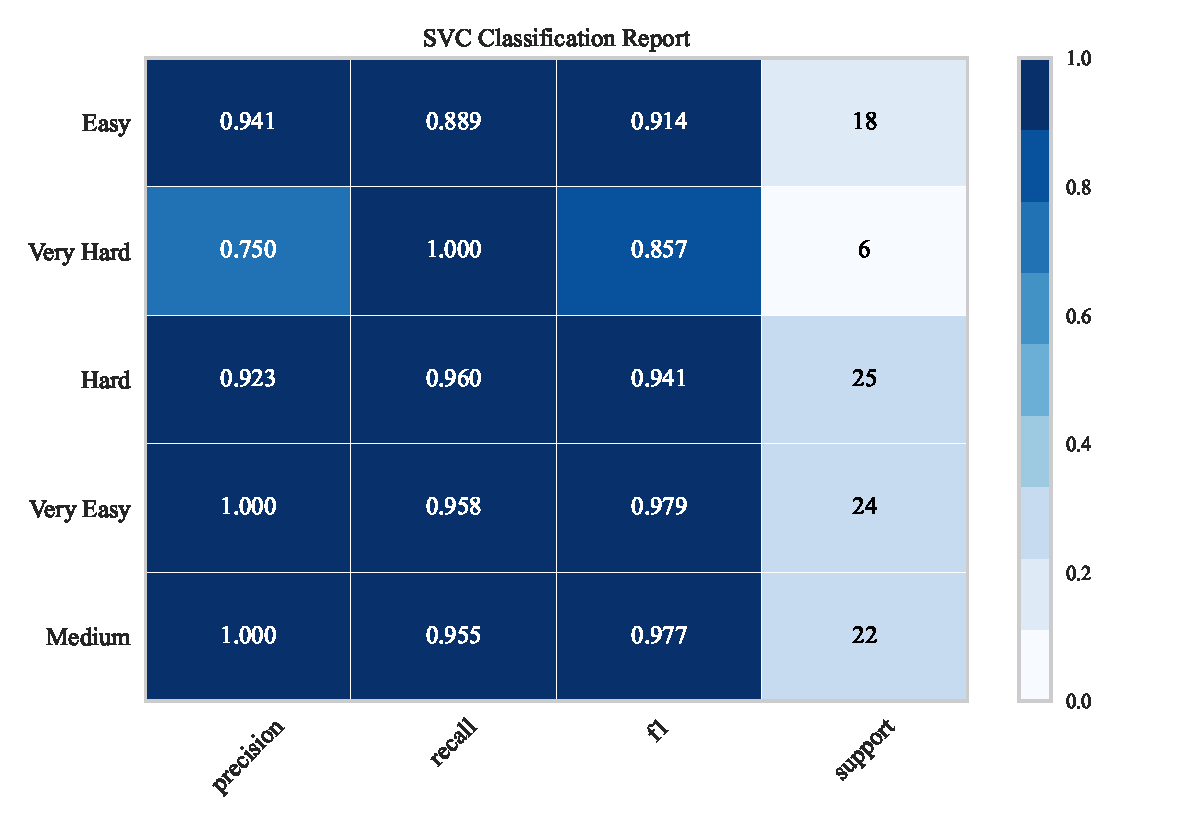
\includegraphics[width=0.90\linewidth]{分类报告.pdf}
				\caption{分类报告}
				\label{fig:分类报告}
			\end{minipage}
		\end{figure}

		观察该图,我们可以发现,该模型对于预测单词难度具有较好的效果,主对角线附近元素较多,说明模型预测正确的误差较小,预测难度与实际难度非常接近,可以较好分类单词难度。

		\item \textbf{分类报告(Classification Report)}。分类报告图示可以直观得到模型各项参数,包括每一类别的精确率(Precision),召回率(Recall),F1分数值(F1-Score)。对于这三项值,其计算公式如下:
		\begin{itemize}
			\item {\heiti 精确率}
			\begin{equation}
				\mathrm{Precision} = \frac{TP}{TP+FP} \label{Precision}
			\end{equation}
			\item {\heiti 召回率}
			\begin{equation}
				\mathrm{Recall} = \frac{TP}{TP+FN} \label{Recall}
			\end{equation}
			\item {\heiti F1分数值} 
			\begin{equation}
				\mathrm{F}1 = \frac{2\times \mathrm{Precision}\times \mathrm{Recall}}{\mathrm{Precision}+\mathrm{Recall}}=\frac{TP}{TP+\frac{1}{2}\left(FP+FN\right)} \label{F1-Score}
			\end{equation}
		\end{itemize}
		根据上述\textcolor{blue}{\eqref{Precision}}、\textcolor{blue}{\eqref{Recall}}、\textcolor{blue}{\eqref{F1-Score}},我们可以计算出每一个模型对于每一类别的三项指标值,并绘制分类报告图,见\textcolor{blue}{\cref{fig:分类报告}}。

		此外,对于模型的精确率、召回率,我们可以根据定义可以发现若这两项值较大,则模型效果较好。同时根据定义,我们可以发现模型的精确率、召回率在理想情况下是相差较小的,我们可以根据图示结果验证,符合预期效果。对于模型的F1分数值,其为精确率与召回率的调和平均数,因此当精确率与召回率均有较好表现时,F1分数值会有较优秀表现。我们也可对\textcolor{blue}{\eqref{F1-Score}}进行一定变换,可以得到
		\begin{equation}
			\mathrm{F}1=\frac{2}{\dfrac{1}{\mathrm{Precision}}+\dfrac{1}{\mathrm{Recall}}} \label{ReacllNew}
		\end{equation}
		根据该式,我们可以得出上述结论。

		\item \textbf{ROC/AUC(特征曲线及曲线下面积(Receiver Operating Characteristic\\/Area Under the Curve,ROC/AUC)曲线}。在分析该图之前,我们需要了解模型的相关参数,定义如下:
		\begin{itemize}
			\item {\heiti 灵敏度}\textbf{(Sensitivity)}。灵敏度又被称为真阳性率,即$TP$率,定义为:
			\begin{equation}
				\mathrm{Sensitivity}=TPR=\frac{TP}{TP+FN} \label{Sensitivity}
			\end{equation}
			\item {\heiti 特异性}\textbf{(Specificity)}。特异性又被称为真阴性率,即$TN$率,定义为:
			\begin{equation}
				\mathrm{Specificity}=TNR=\frac{TN}{TN+FP} \label{Specificity}
			\end{equation}
			\item \textbf{1-Specificity}。称为假阳性率(False Positive Rate, $FPR$),定义为:
			\begin{equation}
				FPR=1-\mathrm{Specificity}=\frac{FP}{FP+TN} \label{FPR}
			\end{equation}
			\item \textbf{1-Sensitivity}。称为假阴性率(False Negative Rate, $FNR$),定义为:
			\begin{equation}
				FNR=1-\mathrm{Sensitivity}=\frac{FN}{FN+TP} \label{FNR}
			\end{equation}
		\end{itemize}
		$FPR$和$FNR$均对数据分布的变化不敏感\textcolor{blue}{\cite{procauc}},因此这两个指标可以用于在不平衡的数据上建立的模型效果的评价。
		
		对于ROC/AUC曲线,其以每一类别的$1-\mathrm{Specificity}$即$FPR$为横坐标,以$\mathrm{Sensitivity}$即$TPR$为纵坐标,其可体现出模型的灵敏度与特异性之间的关系与差异。因此,该图的理想点位于左上角,即$FPR=0$且$TPR=1$,换言之,当曲线越靠近左上角,模型效果就越优。从而,我们可以得到另一项指标,即曲线下面积(Area Under the Curve, AUC),由上述分析可知,AUC值越高,模型的整体效果也就越优。对于模型一的ROC/AUC曲线,见\textcolor{blue}{\cref{fig:ROCAUC曲线}}。

		\begin{figure}[H]
			\centering
			\begin{minipage}{0.48\linewidth}
				\centering
				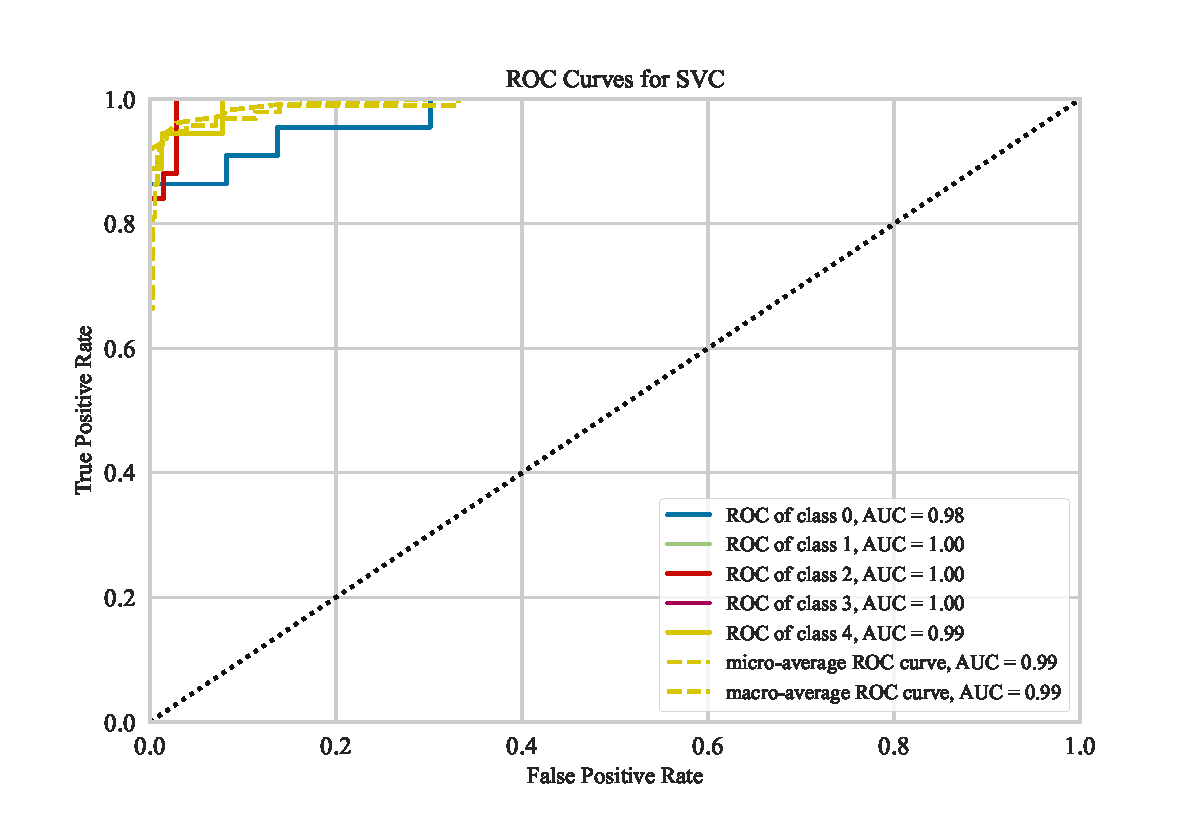
\includegraphics[width=0.95\linewidth]{ROCAUC曲线.pdf}
				\caption{ROC/AUC曲线}
				\label{fig:ROCAUC曲线}
			\end{minipage}
			%\qquad
			\begin{minipage}{0.48\linewidth}
				\centering
				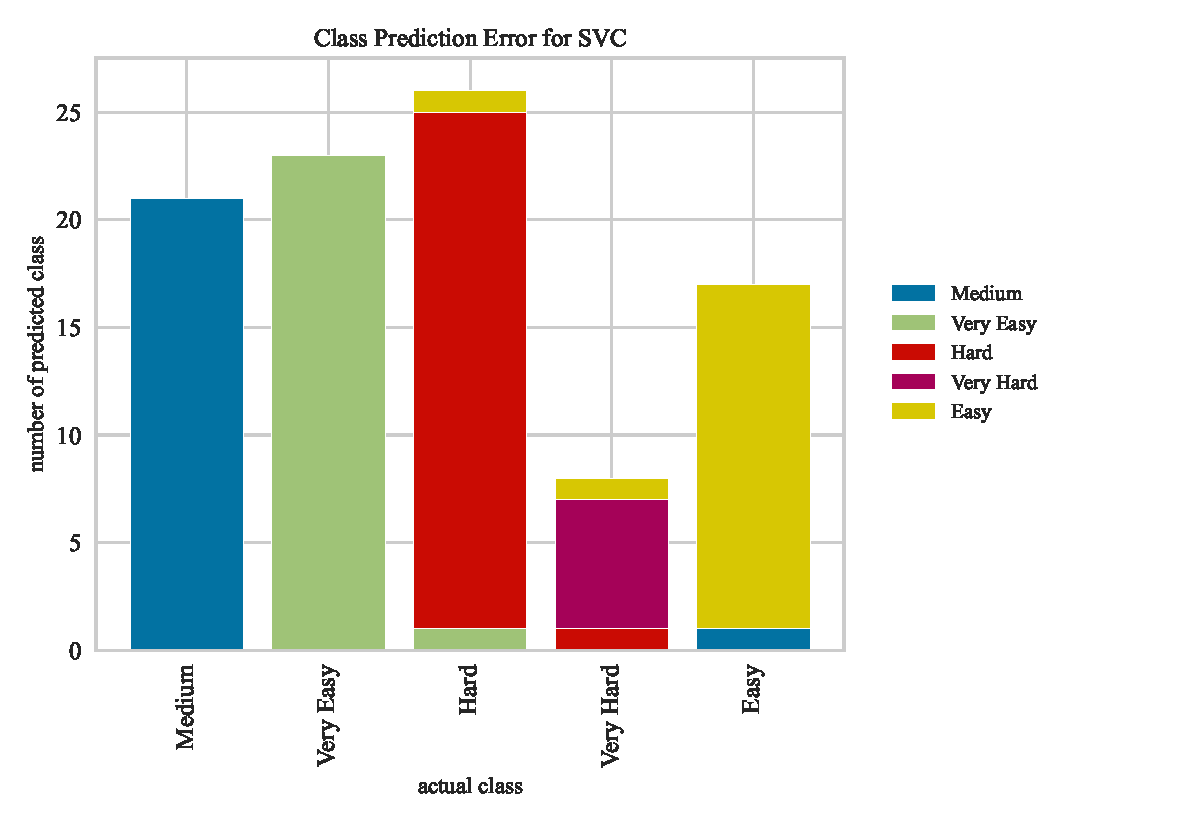
\includegraphics[width=0.90\linewidth]{分类预测结果.pdf}
				\caption{分类预测结果}
				\label{fig:分类预测结果}
			\end{minipage}
		\end{figure}

		根据上图结果,我们可以发现模型对于分类预测单词难度结果中,每一类别的$\text{AUC}$均接近于$1$,曲线下面积较大,可以说明模型整体能力较优。

		\item \textbf{分类预测结果}。如\textcolor{blue}{\cref{fig:分类预测结果}}所示,我们发现在预测结果中只有少部分的数据预测错误,模型的准确度高。
	\end{itemize}
\section{模型的评价与推广}
	\subsection{模型的评价}
	\begin{itemize}
		\item \textbf{模型的优点}:
			\begin{enumerate}
				\item 本文结合游戏生命周期、信息理论等,并且将单词特征分为词性、流行度、信息熵等客观条件,使模型更加具体客观与全面。
				\item 在建立模型前我们通过爬取新数据,并于附件数据合并,增加数据体量,病对数据集进行预处理,使数据更完整且真实,得到的结果更符合实际。
				\item 由于数据的波动性,传统时间序列用于分析效果较差。因此,本文采用XGboost模型准确预测未来报告结果的数量范围,进度较高。
				\item 利用K-means聚类,结合肘部法则,选择最优聚类$k$值,对单词聚类,再依此建立支持向量机SVM多分类预测模型,对难度分类,效果优秀。
				\item 对玩家尝试次数分布进行多模型的拟合分析,通过比较选择随机森林模型进行预测,提高预测精度。
				\item 对模型、数据进行多方面的可视化,提高数据利用率。
			\end{enumerate}
		\item \textbf{模型的缺点及改进}:
			\begin{enumerate}
				\item 在计算词语信息熵的属性时,可以加入词语使用频率来优化信息熵的计算方式,使计算结果更符合实际。
				\item 在进行预测时,可以结合优化算法,如贝叶斯调优进一步优化模型超参数,以提高预测精度。其主要方法为:利用已知的超参数$x$和模型结果$y$来拟合一个代理模型,再利用采集函数选择下一个最优$\left(x,y\right)$,并用此新的$\left(x,y\right)$来优化代理模型,重复上述过程,最终得到调优后的参数,其算法伪代码如\textcolor{blue}{Algorithm \ref{贝叶斯优化}}所示。
			\end{enumerate}
	\end{itemize}

	\scalebox{0.85}{
		\begin{algorithm}[H]
			\label{贝叶斯优化}
			\KwIn{初始化点个数$n_0$,最大迭代次数$N$,代理模型$g\left(x\right)$,采集函数$\alpha\left(x|D\right)$}
			\KwOut{最优候选评估点:$\left\{x^{*},y^{*}\right\}$}
			\textbf{Step 1:}随机初始化$n_0$点$X_{\text{init}}=\left\{x_0,x_1,\cdots,x_{n_0-1}\right\}$\
			
			\textbf{Step 2:}获取其对应的函数值$f\left(X_\text{init}\right)$,初始点集$D_0=\left\{X_\text{init},f\left(X_\text{init}\right)\right\}$,令$t=n_0$,$D_{t-1}=D_0$\

			\While{t<N}{
				\textbf{Step 3:}根据当前获得的点集$D_{t-1}$,构建代理模型$g\left(x\right)$\
				
				\textbf{Step 4:}基于代理模型$g\left(x\right)$,最大化采集函数$\alpha\left(x|D_{t-1}\right)$,获得下一个评估点:$x_t=\text{argmin}\,\alpha\left(x|D_{t-1}\right)$\
				
				\textbf{Step 5:}获得评估点$x_t$的函数值$f\left(x_t\right)$,将其加入到当前评估点集合中:$D_t=D_{t-1}U\left\{x_t,f\left(x_t\right)\right\}$,转\textbf{Step 3}\
			}

			\KwResult{最优候选评估点:$\left\{x^{*},y^{*}\right\}$}
			\caption{贝叶斯优化框架}
		\end{algorithm}}

	\subsection{模型的推广}
	\textbf{其一},XGBoost、随机森林回归模型具有处理多维数据及预测未来结果的能力,因此我们认为,其可应用于金融行业风险预测分析,及时为可能出现的经济危机做出预警,一定程度上避免恶性事件的发生。同时,在医学层面,其也可预测流行性疾病的发展趋势,并为医学专家下一步的疫情防控工作提供帮助。\textbf{其二},K-means聚类与SVM多分类预测模型可较好地分类事物类别,并对未知类别进行预测,因此其有利于基于对现有未分类事物进行聚类,并对新添事物进行类别预测分析,可应用于文物鉴定等领域。总而言之,本文所建立模型有着精度较高、泛化能力较强的优秀品质,可为经济,医学,考古等多行业提供有利帮助。
	\newpage
	\phantomsection
	\addcontentsline{toc}{section}{\textbf{参考文献}}
	\begin{spacing}{1.08}
	\begin{thebibliography}{99}
	\bibitem{pxgboost1}陈振宇,刘金波,李晨,季晓慧,李大鹏,黄运豪,狄方春,高兴宇,徐立中.基于LSTM与XGBoost组合模型的超短期电力负荷预测[J].电网技术,2020,44(02):614-620.DOI:10.13335/j.1000-3673.pst.2019.1566.

	\bibitem{pxgboost2}杨贵军,徐雪,赵富强.基于XGBoost算法的用户评分预测模型及应用[J].数据分析与知识发现,2019,3(01):118-126.

	\bibitem{pxgboost3}Tianqi Chen and Carlos Guestrin. 2016. XGBoost: A Scalable Tree Boosting System. In Proceedings of the 22nd ACM SIGKDD International Conference on Knowledge Discovery and Data Mining (KDD '16). Association for Computing Machinery, New York, NY, USA, 785–794. \url{https://doi.org/10.1145/2939672.2939785}.

	\bibitem{ppearson1}肖杨,李亚,王海瑞,常梦容.基于皮尔逊相关系数的滚动轴承混合域特征选择方法[J].化工自动化及仪表,2022,49(03):308-315.DOI:10.20030/j.cnki.1000-3932.202203009.
	
	\bibitem{ppearson2}王殿武,赵云斌,尚丽英,王凤刚,张震.皮尔逊相关系数算法在B油田优选化学防砂措施井的应用[J].精细与专用化学品,2022,30(07):26-28.DOI:10.19482/j.cn11-3237.2022.07.07.

	\bibitem{psvm}汪海燕,黎建辉,杨风雷.支持向量机理论及算法研究综述[J].计算机应用研究,2014,31(05):1281-1286.

	\bibitem{k-means}CSDN.【零基础学习机器学习】k-means[EO/BL].\url{https://blog.csdn.net/qq_42994177/article/details/105908364}.

	\bibitem{类间距离}Intercluster Distance Maps — Yellowbrick v1.5 documentation[EO/BL].\url{https://www.scikit-yb.org/en/latest/api/cluster/icdm.html#yellowbrick.cluster.icdm.intercluster_distance}.

	\bibitem{procauc}A.Tharwat, Applied Computing and Informatics (2018). \url{https://doi.org/10.1016/j.aci.2018.08.003}.

	\end{thebibliography}
	\end{spacing}
	\newpage

	\phantomsection
	\addcontentsline{toc}{section}{\textbf{附\hspace{2pc}录}}

	% \appendix
	% \ctexset{section={format={\zihao{-4}\heiti\raggedright}}}
	\begin{center}
		\heiti\zihao{4} 附\hspace{2pc}录
	\end{center}

% \phantomsection
% \addcontentsline{toc}{subsection}{[A]图示}
	% \section*{[A]图示}
	\noindent{\heiti [A]图示}
	\begin{figure}[H]
		\centering
		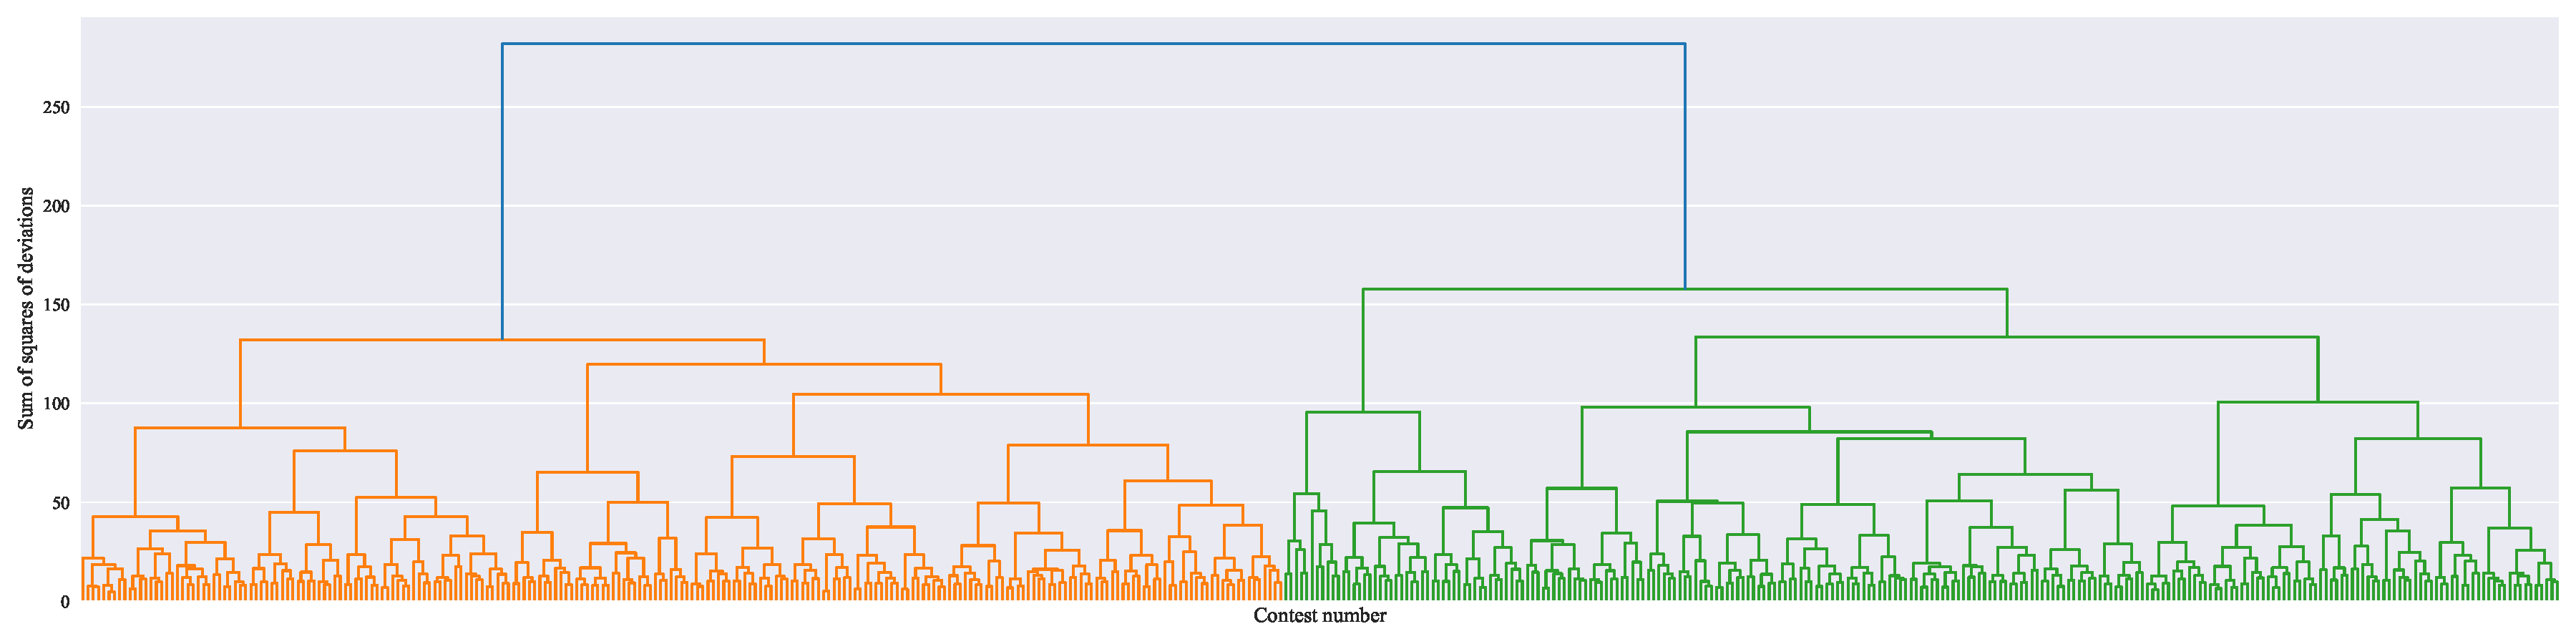
\includegraphics[width=0.95\linewidth]{层次聚类树状图.pdf}
		\caption{层次聚类树状图}
		\label{fig:层次聚类树状图}
	\end{figure}
% \newpage
% \phantomsection
% \addcontentsline{toc}{subsection}{[B]支撑文件列表}
	% \section*{[B]支撑文件列表}
	\noindent{\heiti [B]支撑文件列表}
	~\\

	支撑文件列表如下(按文件夹进行分类):

\begin{table}[H]   
	\centering     
	\begin{tabular}{cc}     
		\toprule     
		\textbf{文件夹名} & \textbf{描述} \\     
		\midrule     
		Code  & 解决问题所有源程序,包括ipynb及其对应的py文件 \\     Figures & 论文中所有矢量图示,均为pdf文件 \\     
		Data  & 解决问题所用数据,均为xlsx文件 \\     
		Result & 程序输出结果,均为html文件 \\     
		\bottomrule     
	\end{tabular}
\end{table}

\newpage
	\noindent{\heiti [C]使用的软件、环境}
	~\\

	\textbf{C.1}:为解决该问题,我们所使用的主要软件有:
	\begin{itemize}
		\item TeX Live 2022
		\item Visual Studio Code 1.77.3
		\item WPS Office 2023春季更新(14036)
		\item Python 3.10.4
		\item Pycharm 2023.1.1 (Professional Edition)
	\end{itemize}

	\textbf{C.2}:Python环境下所用使用到的库及其版本如下:
\begin{table}[H]
	\centering
	\setlength{\aboverulesep}{0pt}
	\setlength{\belowrulesep}{0pt}
	\scalebox{0.90}{
	  \begin{tabular}{cc||cc}
	  \toprule
	  \textbf{库} & \textbf{版本} & \textbf{库} & \textbf{版本} \\
	  \midrule
	  copy  & 内置库   & matplotlib & 3.5.2 \\
	  jupyter & 1.0.0 & nltk  & 3.7 \\
	  jupyter-client & 7.3.1 & numpy & 1.22.4+mkl \\
	  jupyter-console & 6.4.3 & openpyxl & 3.0.10 \\
	  jupyter-contrib-core & 0.4.0 & pandas & 1.4.2 \\
	  jupyter-contrib-nbextensions & 0.5.1 & scikit-learn & 0.22.2 psot1 \\
	  jupyter-highlight-selected-word & 0.2.0 & seaborn & 0.11.2 \\
	  jupyterlab-pygments & 0.2.2 & sklearn & 0 \\
	  jupyterlab-widgets & 1.1.0 & xgboost & 1.6.1 \\
	  jupyter-latex-envs & 1.4.6 & yellowbrick & 1.4 \\
	  jupyter-nbextensions-configurator & 0.5.0 &       &  \\
	  \bottomrule
	  \end{tabular}}
\end{table}
  
\newpage

\noindent{\heiti [D]问题解决源程序}

\textbf{D.1 DataPreProcessing}
\begin{python}
#!/usr/bin/env python
# coding: utf-8

# In[1]:


import pandas as pd
data=pd.read_excel("Data_Wordle.xlsx",sheet_name="Sheet1")
data


# In[2]:


data['Date']=pd.to_datetime(data['Date'])
data.sort_values(by='Date',inplace=True)
data=data.reset_index(drop=True)
data


# In[3]:


import matplotlib.pyplot as plt
plt.rcParams['font.sans-serif'] = ['Times New Roman']
plt.rcParams['axes.unicode_minus'] = False
ax=data.plot(x='Date', y=['Number of reported results', 'Number in hard mode'])
plt.xticks(fontsize=12)
plt.yticks(fontsize=12)
plt.xlabel('Date',fontsize=14)
plt.ylabel('Person Quantity',fontsize=14)
plt.legend()
plt.tight_layout()
plt.savefig("figures\\报告结果每日变化.pdf")


# In[4]:


data['WordLength'] = data['Word'].apply(len)
data['SumRate']=data.loc[:,['1 try','2 tries','3 tries','4 tries','5 tries','6 tries','7 or more tries (X)']].sum(axis=1)
data['HardRate']=data['Number in hard mode']/data['Number of reported results']
data


# In[5]:


data[data['WordLength']!=5]


# In[6]:


ax=data.plot.scatter(x='Date', y='HardRate')
plt.xticks(fontsize=12)
plt.yticks(fontsize=12)
plt.xlabel('Date',fontsize=14)
plt.ylabel('Hard mode frequency',fontsize=14)
plt.tight_layout()
plt.savefig('figures\\每日选择困难模式人数频率变化.pdf')


# In[7]:


data['HardRateDiff']=data['HardRate'].diff()


# In[8]:


data.plot.scatter(x='Date', y='HardRateDiff',color='g')
plt.xticks(fontsize=12)
plt.yticks(fontsize=12)
plt.xlabel('Date',fontsize=14)
plt.ylabel('Hard mode frequency gradient',fontsize=14)
plt.tight_layout()
plt.savefig('figures\\每日选择困难模式人数频率变化率.pdf')


# In[9]:


data=data.fillna(0)
data


# In[10]:


data[abs(data['HardRateDiff'])>=0.02]


\end{python}
\newpage
\textbf{D.2 CreateFeatures}
\begin{python}
#!/usr/bin/env python
# coding: utf-8

# In[1]:


import pandas as pd
import nltk


# In[2]:


data = pd.read_excel("Data_Wordle_All.xlsx", sheet_name="Sheet1")
data


# In[3]:


data['Letters']=data['Word'].apply(lambda x:str(list(x))[1:-1].replace("'","").replace(" ",""))
data['w1'],data['w2'],data['w3'],data['w4'],data['w5']=data['Letters'].str.split(',',n=4).str
letter = [str(chr(i)) for i in range(ord('a'),ord('z')+1)]
letter_map = dict(zip(letter,range(1,27)))
data['w1'] = data['w1'].map(letter_map)
data['w2'] = data['w2'].map(letter_map)
data['w3'] = data['w3'].map(letter_map)
data['w4'] = data['w4'].map(letter_map)
data['w5'] = data['w5'].map(letter_map)
data


# In[4]:


Vowel = ['a','e','i','o','u']
Consonant = list(set(letter).difference(set(Vowel)))


def count_vowel(s):
    c = 0
    for i in range(len(s)):
        if s[i] in Vowel:
            c+=1
    return c


def count_consonant(s):
    c = 0
    for i in range(len(s)):
        if s[i] in Consonant:
            c+=1
    return c


data['Vowel_fre'] = data['Word'].apply(lambda x:count_vowel(x))
data['Consonant_fre'] = data['Word'].apply(lambda x:count_consonant(x))
data


# In[5]:


pos_tags = nltk.pos_tag(list(data['Word']))
data['Speech']=pd.DataFrame(pos_tags)[1]
data


# In[6]:


def count_same_letter(s):
    d={}
    for char in set(s):
        d[char]=s.count(char)

    sum = 0
    for i in d:
        if d[i]>1:
            sum = sum + d[i]

    return sum


# In[7]:


data['Same_letter_fre'] = data['Word'].apply(lambda x:count_same_letter(x))
data


# In[8]:


Frequency=pd.read_excel("Letter_Frequency.xlsx",sheet_name="Sheet1")
Frequency_map=dict(zip(Frequency['N'],Frequency['Frequency']))
data['w1_fre']=data['w1']
data['w2_fre']=data['w2']
data['w3_fre']=data['w3']
data['w4_fre']=data['w4']
data['w5_fre']=data['w5']
data.replace({'w1_fre':Frequency_map,'w2_fre':Frequency_map,'w3_fre':Frequency_map,'w4_fre':Frequency_map,'w5_fre':Frequency_map},inplace=True)
data


# In[9]:


import sklearn.preprocessing as sp
le=sp.LabelEncoder()
data['Speech']=le.fit_transform(data['Speech'])
data


\end{python}
\newpage
\textbf{D.3 IssueOne-1}
\begin{python}
#!/usr/bin/env python
# coding: utf-8

# In[1]:


import pandas as pd
import seaborn as sns
data=pd.read_excel("Data_Wordle_New.xlsx",sheet_name="Sheet1")
data


# In[2]:


import matplotlib.pyplot as plt
plt.rcParams['font.sans-serif'] = ['Times New Roman']
plt.rcParams['axes.unicode_minus'] = False


# In[3]:


sns.set_style('ticks')
ax=sns.jointplot(x=data['Contest number'],y=data['Number of reported results'],kind='kde',height=4,shade=True).plot_joint(sns.regplot,scatter=True,color='#FF3333')
plt.tight_layout()
plt.savefig('figures\\核密度估计值.pdf')


# In[4]:


import scipy.stats as st
import matplotlib.pyplot as plt

plt.figure(figsize=(16, 6))
y = data['Number of reported results']
plt.subplot(121)
sns.distplot(y, kde=False, fit=st.johnsonsu, color='Red')
plt.xticks(font='Times New Roman',fontsize=12)
plt.yticks(font='Times New Roman',fontsize=12)
plt.xlabel('Number of reported results',font='Times New Roman',fontsize=14)

plt.subplot(122)
st.probplot(y, dist="norm", plot=plt)
plt.xticks(font='Times New Roman',fontsize=12)
plt.yticks(font='Times New Roman',fontsize=12)
plt.xlabel('Theoretical quantiles',font='Times New Roman',fontsize=14)
plt.ylabel('Ordered Values',font='Times New Roman',fontsize=14)
plt.title('Probability Plot',font='Times New Roman',fontsize=16)

plt.tight_layout()
plt.savefig("figures\\正态分布分析.pdf")


# In[5]:


data=pd.read_excel("Data_Wordle_All.xlsx",sheet_name='Sheet1')
data


# In[6]:


data['Letters']=data['Word'].apply(lambda x:str(list(x))[1:-1].replace("'","").replace(" ",""))
data['w1'],data['w2'],data['w3'],data['w4'],data['w5']=data['Letters'].str.split(',',n=4).str
letter = [str(chr(i)) for i in range(ord('a'),ord('z')+1)]
letter_map = dict(zip(letter,range(1,27)))
data['w1'] = data['w1'].map(letter_map)
data['w2'] = data['w2'].map(letter_map)
data['w3'] = data['w3'].map(letter_map)
data['w4'] = data['w4'].map(letter_map)
data['w5'] = data['w5'].map(letter_map)
data


# In[7]:


X1=data['Contest number']
y1=data['Number of reported results']


# In[8]:


from sklearn.model_selection import train_test_split
X1_train,X1_test,y1_train,y1_test=train_test_split(X1,y1,test_size=0.1,random_state=20222023)


# In[9]:


from sklearn.metrics import mean_squared_error, mean_absolute_error
from sklearn.metrics import r2_score
import xgboost as xgb

XGB_All = xgb.XGBRegressor(objective='reg:squarederror',n_estimators=100,
                           max_depth=9,learning_rate=0.1,
                           subsample=0.8,reg_lambda= 0.5,
                           reg_alpha= 0,gamma= 0,
                           colsample_bytree=0.6,min_child_weight=5)
XGB_All.fit(X1_train,y1_train)
pre_All=XGB_All.predict(X1)


# In[10]:


mae = mean_absolute_error(data['Number of reported results'], pre_All)
mse = mean_squared_error(data['Number of reported results'], pre_All)
rmse = mse**(1/2)
r2=r2_score(data['Number of reported results'], pre_All)


# In[11]:


print(mae,mse,rmse,r2)


# In[12]:


plt.rcParams['font.sans-serif'] = ['Times New Roman']


# In[13]:


data['Number of reported results Pre']=pre_All
plt.figure(figsize=(8, 6))
data.plot(x='Contest number', y=['Number of reported results', 'Number of reported results Pre'])
plt.xticks(fontsize=12)
plt.yticks(fontsize=12)
plt.xlabel('Contest number',fontsize=14)
plt.ylabel('Number of reported results',fontsize=14)
plt.tight_layout()
plt.savefig('figures\\XGBoost预测结果(总人数).pdf')


# In[14]:


X2=data[['Contest number','Number of reported results']]
y2=data['Number in hard mode']
X2_train,X2_test,y2_train,y2_test=train_test_split(X2,y2,test_size=0.1,random_state=20222023)
XGB_Hard = xgb.XGBRegressor(objective='reg:squarederror',n_estimators=100,
                            max_depth=9,learning_rate=0.1,
                            subsample=0.8,reg_lambda= 0.5,
                            reg_alpha= 0,gamma= 0,
                            colsample_bytree=0.6,min_child_weight=5)
XGB_Hard.fit(X2_train,y2_train)
pre_Hard=XGB_Hard.predict(X2)


# In[15]:


mae = mean_absolute_error(data['Number in hard mode'], pre_Hard)
mse = mean_squared_error(data['Number in hard mode'], pre_Hard)
rmse = mse**(1/2)
r2=r2_score(data['Number in hard mode'], pre_Hard)
print(mae,mse,rmse,r2)


# In[16]:


data['Number in hard mode Pre']=pre_Hard
plt.figure(figsize=(8, 6))
data.plot(x='Contest number', y=['Number in hard mode', 'Number in hard mode Pre'])
plt.xticks(fontsize=12)
plt.yticks(fontsize=12)
plt.xlabel('Contest number',fontsize=14)
plt.ylabel('Number in hard mode',fontsize=14)
plt.tight_layout()
plt.savefig('figures\\XGBoost预测结果(困难人数).pdf')


# In[17]:


import yellowbrick
yellowbrick.style.rcmod.set_aesthetic(font='Times New Roman',font_scale=2)


# In[18]:


from yellowbrick.regressor import PredictionError
model = PredictionError(XGB_All)
model.fit(X1_train, y1_train)
model.score(X1_test, y1_test)
model.poof(outpath='figures\\XGBoost预测误差(总人数).pdf')


# In[19]:


from yellowbrick.regressor import PredictionError
model = PredictionError(XGB_Hard)
model.fit(X2_train, y2_train)
model.score(X2_test, y2_test)
model.poof(outpath='figures\\XGBoost预测误差(困难人数).pdf')


# In[20]:


EERIE_Pre_All=pd.read_excel("EERIE_Pre.xlsx",sheet_name='All')
EERIE_Pre_All


# In[21]:


X_pre_all=XGB_All.predict(EERIE_Pre_All['Contest number'])
X_pre_all


# In[22]:


EERIE_Pre_Hard=pd.read_excel("EERIE_Pre.xlsx",sheet_name='Hard')
EERIE_Pre_Hard


# In[23]:


X_pre_hard=XGB_Hard.predict(EERIE_Pre_Hard[['Contest number','Number of reported results']])
X_pre_hard


\end{python}
\newpage
\textbf{D.4 IssueOne-2}
\begin{python}
#!/usr/bin/env python
# coding: utf-8

# In[1]:


import pandas as pd
import matplotlib.pyplot as plt
import seaborn as sns


# In[2]:


data = pd.read_excel("Data_Wordle_All_Features.xlsx", sheet_name="Data_Wordle_All_Features")
data


# In[3]:


X=data[['1 try','2 tries','3 tries','4 tries','5 tries','6 tries','7 or more tries (X)','w1','w2','w3','w4','w5','Vowel_fre','Consonant_fre','Same_letter_fre','Speech','w1_fre','w2_fre','w3_fre','w4_fre','w5_fre']]
X


# In[4]:


plt.subplots(figsize = (21, 21))
sns.heatmap(X.corr(method='pearson'),linewidths=0.1,vmax=1.0,square=True,linecolor='white',annot=True,annot_kws={'size':12})
plt.rcParams['font.sans-serif']=['Times New Roman']
plt.rcParams['axes.unicode_minus']=False
plt.xticks(fontsize=14)
plt.yticks(fontsize=14)
plt.title('Pearson\'s correlation coefficient', size=16)
plt.savefig('figures\\皮尔逊相关系数.pdf',bbox_inches='tight')


\end{python}
\newpage
\textbf{D.5 IssueTwo}
\begin{python}
#!/usr/bin/env python
# coding: utf-8

# In[1]:


import pandas as pd
data=pd.read_excel('Data_Wordle_All_Features.xlsx',sheet_name='Data_Wordle_All_Features')
data


# In[2]:


features = ['Contest number','Number of reported results','Number in hard mode','w1','w2','w3','w4','w5','w1_fre','w2_fre','w3_fre','w4_fre','w5_fre','Vowel_fre','Consonant_fre','Speech','Same_letter_fre']
label = ['1 try','2 tries','3 tries','4 tries','5 tries','6 tries','7 or more tries (X)']

Train_all = data[features+label].copy().dropna()
X = Train_all[features]

Y_1= Train_all[label[0]]
Y_2= Train_all[label[1]]
Y_3= Train_all[label[2]]
Y_4= Train_all[label[3]]
Y_5= Train_all[label[4]]
Y_6= Train_all[label[5]]
Y_7= Train_all[label[6]]


# In[3]:


from xgboost import XGBRegressor
from sklearn.ensemble import RandomForestRegressor
from lightgbm import LGBMRegressor
from sklearn.metrics import mean_squared_error, mean_absolute_error
from sklearn.metrics import r2_score
from sklearn.model_selection import train_test_split
from sklearn.linear_model import LinearRegression


# In[4]:


def linear(X,y,i):
    X_train, X_test, y_train, y_test = train_test_split(X,y, test_size=0.1, random_state=20222023)
    reg=LinearRegression()
    reg.fit(X_train,y_train)
    pre_all=reg.predict(X)
    mae = mean_absolute_error(data[label[i-1]], pre_all)
    mse = mean_squared_error(data[label[i-1]], pre_all)
    rmse = mse**(1/2)
    r2=r2_score(data[label[i-1]], pre_all)
    print(f'线性回归:尝试{i}次,RMSE:{rmse};MSE:{mse};MAE:{mae};r2:{r2}')


def xgboost(X,y,i):
    X_train, X_test, y_train, y_test = train_test_split(X,y, test_size=0.1, random_state=20222023)
    reg=XGBRegressor()
    reg.fit(X_train,y_train)
    pre_all=reg.predict(X)
    mae = mean_absolute_error(data[label[i-1]], pre_all)
    mse = mean_squared_error(data[label[i-1]], pre_all)
    rmse = mse**(1/2)
    r2=r2_score(data[label[i-1]], pre_all)
    print(f'XGB:尝试{i}次,RMSE:{rmse};MSE:{mse};MAE:{mae};r2:{r2}')


def rf(X,y,i):
    X_train, X_test, y_train, y_test = train_test_split(X,y, test_size=0.1, random_state=20222023)
    reg=RandomForestRegressor()
    reg.fit(X_train,y_train)
    pre_all=reg.predict(X)
    mae = mean_absolute_error(data[label[i-1]], pre_all)
    mse = mean_squared_error(data[label[i-1]], pre_all)
    rmse = mse**(1/2)
    r2=r2_score(data[label[i-1]], pre_all)
    print(f'RF:尝试{i}次,RMSE:{rmse};MSE:{mse};MAE:{mae};r2:{r2}')


def lgbm(X,y,i):
    X_train, X_test, y_train, y_test = train_test_split(X,y, test_size=0.1, random_state=20222023)
    reg=LGBMRegressor(objective='regression', num_leaves=31, learning_rate=0.05, n_estimators=20)
    reg.fit(X_train,y_train)
    pre_all=reg.predict(X)
    mae = mean_absolute_error(data[label[i-1]], pre_all)
    mse = mean_squared_error(data[label[i-1]], pre_all)
    rmse = mse**(1/2)
    r2=r2_score(data[label[i-1]], pre_all)
    print(f'LGBM:尝试{i}次,RMSE:{rmse};MSE:{mse};MAE:{mae};r2:{r2}')


# In[5]:


linear(X,Y_1,1)
linear(X,Y_2,2)
linear(X,Y_3,3)
linear(X,Y_4,4)
linear(X,Y_5,5)
linear(X,Y_6,6)
linear(X,Y_7,7)

xgboost(X,Y_1,1)
xgboost(X,Y_2,2)
xgboost(X,Y_3,3)
xgboost(X,Y_4,4)
xgboost(X,Y_5,5)
xgboost(X,Y_6,6)
xgboost(X,Y_7,7)

rf(X,Y_1,1)
rf(X,Y_2,2)
rf(X,Y_3,3)
rf(X,Y_4,4)
rf(X,Y_5,5)
rf(X,Y_6,6)
rf(X,Y_7,7)

lgbm(X,Y_1,1)
lgbm(X,Y_2,2)
lgbm(X,Y_3,3)
lgbm(X,Y_4,4)
lgbm(X,Y_5,5)
lgbm(X,Y_6,6)
lgbm(X,Y_7,7)


# In[6]:


eerie=pd.read_excel('EERIE.xlsx',sheet_name='Sheet1')
eerie


# In[7]:


import nltk

letter = [str(chr(i)) for i in range(ord('a'),ord('z')+1)]
Vowel = ['a','e','i','o','u']
Consonant = list(set(letter).difference(set(Vowel)))


def count_vowel(s):
    c = 0
    for i in range(len(s)):
        if s[i] in Vowel:
            c+=1
    return c


def count_consonant(s):
    c = 0
    for i in range(len(s)):
        if s[i] in Consonant:
            c+=1
    return c


def count_same_letter(s):
    d={}
    for char in set(s):
        d[char]=s.count(char)

    sum = 0
    for i in d:
        if d[i]>1:
            sum = sum + d[i]

    return sum


eerie['Vowel_fre'] = eerie['Word'].apply(lambda x:count_vowel(x))
eerie['Consonant_fre'] = eerie['Word'].apply(lambda x:count_consonant(x))

pos_tags = nltk.pos_tag(list(eerie['Word']))
eerie['Speech']=pd.DataFrame(pos_tags)[1]
eerie.replace({'Speech':{'NN':7}},inplace=True)

eerie['Same_letter_fre'] = eerie['Word'].apply(lambda x:count_same_letter(x))

letter_map = dict(zip(letter,range(1,27)))
eerie['w1'] = eerie['w1'].map(letter_map)
eerie['w2'] = eerie['w2'].map(letter_map)
eerie['w3'] = eerie['w3'].map(letter_map)
eerie['w4'] = eerie['w4'].map(letter_map)
eerie['w5'] = eerie['w5'].map(letter_map)

Frequency=pd.read_excel("Letter_Frequency.xlsx",sheet_name="Sheet1")
Frequency_map=dict(zip(Frequency['N'],Frequency['Frequency']))
eerie['w1_fre']=eerie['w1']
eerie['w2_fre']=eerie['w2']
eerie['w3_fre']=eerie['w3']
eerie['w4_fre']=eerie['w4']
eerie['w5_fre']=eerie['w5']
eerie.replace({'w1_fre':Frequency_map,'w2_fre':Frequency_map,'w3_fre':Frequency_map,'w4_fre':Frequency_map,'w5_fre':Frequency_map},inplace=True)

eerie


# In[8]:


features = ['Contest number','Number of reported results','Number in hard mode','w1','w2','w3','w4','w5','w1_fre','w2_fre','w3_fre','w4_fre','w5_fre','Vowel_fre','Consonant_fre','Speech','Same_letter_fre']
label = ['1 try','2 tries','3 tries','4 tries','5 tries','6 tries','7 or more tries (X)']
Train_all = data[features+label].copy().dropna()
X = Train_all[features]

Y_1=Train_all[label[0]]
Y_2=Train_all[label[1]]
Y_3=Train_all[label[2]]
Y_4=Train_all[label[3]]
Y_5=Train_all[label[4]]
Y_6=Train_all[label[5]]
Y_7=Train_all[label[6]]

reg1 = XGBRegressor(random_state=20222023).fit(X, Y_1)
reg2 = XGBRegressor(random_state=20222023).fit(X, Y_2)
reg3 = XGBRegressor(random_state=20222023).fit(X, Y_3)
reg4 = XGBRegressor(random_state=20222023).fit(X, Y_4)
reg5 = XGBRegressor(random_state=20222023).fit(X, Y_5)
reg6 = XGBRegressor(random_state=20222023).fit(X, Y_6)
reg7 = XGBRegressor(random_state=20222023).fit(X, Y_7)

X_pred=eerie[features]
p_pred1 = reg1.predict(X_pred)
p_pred2 = reg2.predict(X_pred)
p_pred3 = reg3.predict(X_pred)
p_pred4 = reg4.predict(X_pred)
p_pred5 = reg5.predict(X_pred)
p_pred6 = reg6.predict(X_pred)
p_pred7 = reg7.predict(X_pred)

print(p_pred1,p_pred2,p_pred3,p_pred4,p_pred5,p_pred6,p_pred7)


# In[9]:


features = ['Contest number','Number of reported results','Number in hard mode','w1','w2','w3','w4','w5','w1_fre','w2_fre','w3_fre','w4_fre','w5_fre','Vowel_fre','Consonant_fre','Speech','Same_letter_fre']
label = ['1 try','2 tries','3 tries','4 tries','5 tries','6 tries','7 or more tries (X)']
Train_all = data[features+label].copy().dropna()
X = Train_all[features]

Y_1= Train_all[label[0]]
Y_2= Train_all[label[1]]
Y_3= Train_all[label[2]]
Y_4= Train_all[label[3]]
Y_5= Train_all[label[4]]
Y_6= Train_all[label[5]]
Y_7= Train_all[label[6]]

reg1 = RandomForestRegressor(random_state=202305).fit(X, Y_1)
reg2 = RandomForestRegressor(random_state=202305).fit(X, Y_2)
reg3 = RandomForestRegressor(random_state=202305).fit(X, Y_3)
reg4 = RandomForestRegressor(random_state=202305).fit(X, Y_4)
reg5 = RandomForestRegressor(random_state=202305).fit(X, Y_5)
reg6 = RandomForestRegressor(random_state=202305).fit(X, Y_6)
reg7 = RandomForestRegressor(random_state=202305).fit(X, Y_7)

X_pred=eerie[features]
p_pred1 = reg1.predict(X_pred)
p_pred2 = reg2.predict(X_pred)
p_pred3 = reg3.predict(X_pred)
p_pred4 = reg4.predict(X_pred)
p_pred5 = reg5.predict(X_pred)
p_pred6 = reg6.predict(X_pred)
p_pred7 = reg7.predict(X_pred)
print(p_pred1,p_pred2,p_pred3,p_pred4,p_pred5,p_pred6,p_pred7)


# In[10]:


from yellowbrick.regressor import ResidualsPlot
import matplotlib.pyplot as plt
plt.rcParams['font.sans-serif'] = ['Times New Roman']
Xt_train, Xt_test, yt_train, yt_test = train_test_split(X,Y_4, test_size=0.1, random_state=20222023)
model = ResidualsPlot(RandomForestRegressor(random_state=202305))
model.fit(Xt_train, yt_train)
model.score(Xt_test, yt_test)
model.poof(outpath="figures\\预测残差图-4.pdf")


\end{python}
\newpage
\textbf{D.6 IssueThree}
\begin{python}
#!/usr/bin/env python
# coding: utf-8

# In[1]:


import pandas as pd
data=pd.read_excel('Data_Wordle_All_Features.xlsx',sheet_name='Data_Wordle_All_Features')
data


# In[2]:


dataNew=data[['1 try','2 tries','3 tries','4 tries','5 tries','6 tries','7 or more tries (X)','w1','w2','w3','w4','w5','Vowel_fre','Consonant_fre','Speech','Same_letter_fre','w1_fre','w2_fre','w3_fre','w4_fre','w5_fre']]


# In[3]:


import scipy.cluster.hierarchy as sch
import matplotlib.pyplot as plt
plt.figure(figsize=(24, 6))
dendrogram = sch.dendrogram(sch.linkage(dataNew, method = 'ward'))
plt.rcParams['font.sans-serif']=['Times New Roman']
plt.rcParams['axes.unicode_minus']=False
plt.xlabel('Contest number',fontsize=14)
plt.ylabel('Sum of squares of deviations',fontsize=14)
plt.xticks([],font='Times New Roman',fontsize=12)
plt.yticks(font='Times New Roman',fontsize=12)
plt.tight_layout()
plt.savefig("figures\\层次聚类树状图.pdf")


# In[4]:


from yellowbrick.cluster import KElbowVisualizer
from sklearn.cluster import KMeans
from sklearn.metrics import silhouette_score
from yellowbrick.cluster import InterclusterDistance
from yellowbrick.cluster import SilhouetteVisualizer


# In[5]:


model = KElbowVisualizer(KMeans(random_state = 20222023), k=12)
model.fit(dataNew)
model.poof(outpath="figures\\肘部法则.pdf")


# In[6]:


n_clusters = 5
cluster = KMeans(n_clusters = n_clusters, random_state = 20222023).fit(dataNew)
y_pred = cluster.labels_
data['Class']=y_pred
data


# In[7]:


# 输出5个类别数据
def ClassDataOutPut(i):
    data[data['Class']==i].to_excel(f'Class\\Class {i}.xlsx',sheet_name='Class')


for i in range(5):
    ClassDataOutPut(i)


# In[8]:


silhouette_score(dataNew, y_pred)


# In[9]:


model = SilhouetteVisualizer(cluster)
model.fit(dataNew)
model.poof(outpath='figures\\轮廓系数.pdf')


# In[10]:


model = InterclusterDistance(cluster)
model.fit(dataNew)
model.poof(outpath='figures\\类间距离.pdf')


# In[11]:


from sklearn.decomposition import PCA
pca = PCA(n_components=2)
DataNewPCA = pca.fit_transform(dataNew)
x0, y0= [], []
x1, y1= [], []
x2, y2= [], []
x3, y3= [], []
x4, y4= [], []

plt.rcParams['font.sans-serif'] = ['Times New Roman']
plt.rcParams['axes.unicode_minus'] = False

for index, value in enumerate(y_pred):
    if value == 0:
        x0.append(DataNewPCA[index][0])
        y0.append(DataNewPCA[index][1])
    elif value == 1:
        x1.append(DataNewPCA[index][0])
        y1.append(DataNewPCA[index][1])
    elif value == 2:
        x2.append(DataNewPCA[index][0])
        y2.append(DataNewPCA[index][1])
    elif value == 3:
        x3.append(DataNewPCA[index][0])
        y3.append(DataNewPCA[index][1])
    elif value == 4:
        x4.append(DataNewPCA[index][0])
        y4.append(DataNewPCA[index][1])

plt.figure(figsize=(10, 10))

# #定义坐标轴
k = 200
plt.scatter(x0, y0,s=k)
plt.scatter(x1, y1,s=k)
plt.scatter(x2, y2,s=k)
plt.scatter(x3, y3,s=k)
plt.scatter(x4, y4,s=k)
plt.legend(['Medium','Very Easy','Hard','Very Hard','Easy'])
plt.xticks(fontsize=12)
plt.yticks(fontsize=12)
plt.xlabel('PC2',fontsize=14)
plt.ylabel('PC1',fontsize=14)
plt.tight_layout()
plt.savefig('figures\\聚类散点图.pdf')


# In[12]:


EERIE=pd.read_excel("EERIE_Result(Initially+EERIE&EERIE).xlsx",sheet_name='EERIE_Result')
EERIE


# In[13]:


data


# In[14]:


X=data[['1 try','2 tries','3 tries','4 tries','5 tries','6 tries','7 or more tries (X)','w1','w2','w3','w4','w5','Vowel_fre','Consonant_fre','Speech','Same_letter_fre','w1_fre','w2_fre','w3_fre','w4_fre','w5_fre']]
X


# In[15]:


from sklearn.model_selection import train_test_split
from sklearn.svm import SVC
y=data['Class']
X_train, X_test, y_train, y_test = train_test_split(X, y, test_size=0.2, random_state=20222023)
SVM = SVC(random_state=20222023)
SVM.fit(X_train, y_train)
SVM_score = SVM.score(X_test, y_test)
SVM_score


# In[16]:


SVM.predict(EERIE[['1 try','2 tries','3 tries','4 tries','5 tries','6 tries','7 or more tries (X)','w1','w2','w3','w4','w5','Vowel_fre','Consonant_fre','Speech','Same_letter_fre','w1_fre','w2_fre','w3_fre','w4_fre','w5_fre']])


# In[17]:


from yellowbrick.classifier import ConfusionMatrix
classes=['Medium','Very Easy','Hard','Very Hard','Easy']
confusion_matrix = ConfusionMatrix(SVM, classes=classes, cmap='BuGn')
confusion_matrix.fit(X_train, y_train)
confusion_matrix.score(X_test, y_test)
plt.xticks(font='Times New Roman')
plt.yticks(font='Times New Roman')
confusion_matrix.show(outpath='figures\\混淆矩阵热力图.pdf')


# In[18]:


from yellowbrick.classifier import ClassificationReport
visualizer = ClassificationReport(SVM, classes=classes, support=True, cmap='Blues')
visualizer.fit(X_train, y_train)
visualizer.score(X_test, y_test)
plt.xticks(font='Times New Roman')
plt.yticks(font='Times New Roman')
visualizer.show(outpath='figures\\分类报告.pdf')


# In[19]:


from yellowbrick.classifier import ROCAUC
visualizer = ROCAUC(SVM)
visualizer.fit(X_train, y_train)
visualizer.score(X_test, y_test)
plt.xticks(font='Times New Roman')
plt.yticks(font='Times New Roman')
visualizer.show(outpath='figures\\ROCAUC曲线.pdf')


# In[20]:


from yellowbrick.classifier import ClassPredictionError
visualizer = ClassPredictionError(SVM, classes=classes)
visualizer.fit(X_train, y_train)
visualizer.score(X_test, y_test)
plt.xticks(font='Times New Roman')
plt.yticks(font='Times New Roman')
visualizer.show(outpath='figures\\分类预测结果.pdf')


\end{python}
\newpage
\textbf{D.7 IssueFour}
\begin{python}
#!/usr/bin/env python
# coding: utf-8

# In[1]:


from itertools import cycle
import matplotlib.pyplot as plt
import pandas as pd
import nltk
data=pd.read_excel("WordleClass.xlsx",sheet_name='ALL')
data


# In[2]:


plt.rcParams['font.sans-serif']=['Times New Roman']


# In[3]:


def dclass(s):
    if s==0:
        return 'Medium'
    elif s==1:
        return 'Very Easy'
    elif s==2:
        return 'Hard'
    elif s==3:
        return 'Very Hard'
    elif s==4:
        return 'Easy'


data['Class']=data['Class'].apply(dclass)

data['Average Tries']=(1*data['1 try']+2*data['2 tries']+3*data['3 tries']+4*data['4 tries']+5*data['5 tries']+6*data['6 tries']+7*data['7 or more tries (X)'])/100

pos_tags = nltk.pos_tag(list(data['Word']))
data['Speech']=pd.DataFrame(pos_tags)[1]

data['Letter average frequency']=(data['w1_fre']+data['w2_fre']+data['w3_fre']+data['w4_fre']+data['w5_fre'])/5

data


# In[4]:


data['Speech'].value_counts()


# In[5]:


groups = data.groupby('Class')
markers = ['1', 'x', '.','+','*']

fig, ax = plt.subplots()
for (name, group), marker in zip(groups, cycle(markers)):
    ax.plot(group.Date, group['Number of reported results'], marker=marker, linestyle='', ms=5, label=name)
ax.legend()
plt.xlabel('Date',fontsize=14)
plt.ylabel('Number of reported results',fontsize=14)
plt.savefig('figures\\WordleClass.pdf')


# In[6]:


data['Hard Rate']=data['Number in hard mode']/data['Number of reported results']
ax=data.plot.scatter(x='Date', y='Hard Rate')
plt.xticks(fontsize=12)
plt.yticks(fontsize=12)
plt.xlabel('Date',fontsize=14)
plt.ylabel('Hard mode frequency',fontsize=14)
plt.tight_layout()
plt.savefig('figures\\选择困难游戏模式游戏的人数比例.pdf')


# In[7]:


import seaborn as sns
sns.set_style('ticks')
ax=sns.jointplot(x=data['Contest number'],y=data['Hard Rate'],kind='kde',height=4,shade=True).plot_joint(sns.regplot,scatter=True,color='#FF3333')
plt.tight_layout()
plt.savefig('figures\\选择困难游戏模式游戏的人数比例核密度.pdf')


# In[8]:


plt.rcParams['font.sans-serif']=['Times New Roman']
plt.style.use('ggplot')
sns.violinplot(x = "Class",
               y = "Letter average frequency",
               data = data,
               order = ['Very Easy','Easy','Medium','Hard','Very Hard'],
               split = True,)
plt.savefig("figures\\单词字母平均出现率与难度.pdf")


# In[9]:


sns.violinplot(x = "Class",
               y = "Hard Rate",
               data = data,
               order = ['Very Easy','Easy','Medium','Hard','Very Hard'],
               split = True,)
plt.savefig("figures\\选择困难模式占比与难度.pdf")


# In[10]:


sns.violinplot(x = "Speech",
               y = "Hard Rate",
               data = data,
               order = ['NN','JJ','VBP','VBD','RB','VB','NNS','VBN','IN','VBZ'],
               split = True,)
plt.savefig("figures\\选择困难模式占比与词性.pdf")


# In[11]:


sns.violinplot(x = "Class",
               y = "Average Tries",
               data = data,
               order = ['Very Easy','Easy','Medium','Hard','Very Hard'],
               split = True,)
plt.savefig("figures\\平均尝试次数与难度.pdf")


# In[12]:


sns.violinplot(x = "Speech",
               y = "Average Tries",
               data = data,
               order = ['NN','JJ','VBP','VBD','RB','VB','NNS','VBN','IN','VBZ'],
               split = True,)
plt.savefig("figures\\平均尝试次数与词性.pdf")


# In[13]:


sns.violinplot(x = "Vowel_fre",
               y = "Average Tries",
               data = data,
               order = [1,2,3],
               split = True,)
plt.savefig("figures\\平均尝试次数与单词中元音个数.pdf")


# In[14]:


sns.violinplot(x = "Same_letter_fre",
               y = "Average Tries",
               data = data,
               order = [0,2,3,4],
               split = True,)
plt.savefig("figures\\平均尝试次数与单词中相同字母个数.pdf")


# In[15]:


plt.style.use('ggplot')
plt.rcParams['font.sans-serif']=['Times New Roman']
data.plot(x='Contest number',y=['1 try','2 tries','3 tries','4 tries'],figsize=(10,6))
plt.xticks(fontsize=12)
plt.yticks(fontsize=12)
plt.xlabel('Percentage',fontsize=14)
plt.ylabel('Contest number',fontsize=14)
plt.savefig('figures\\尝试次数分布1.pdf')


# In[16]:


data.plot(x='Contest number',y=['5 tries','6 tries','7 or more tries (X)'],figsize=(10,6))
plt.xticks(fontsize=12)
plt.yticks(fontsize=12)
plt.xlabel('Percentage',fontsize=14)
plt.ylabel('Contest number',fontsize=14)
plt.savefig('figures\\尝试次数分布2.pdf')


\end{python}
\newpage
\textbf{D.8 IssueThreeAdd}
\begin{python}
#!/usr/bin/env python
# coding: utf-8

# In[1]:


import matplotlib.pyplot as plt
import pandas as pd
data=pd.read_excel("WordleClass.xlsx",sheet_name='ALL')
data


# In[2]:


from yellowbrick.features import RadViz
from sklearn.model_selection import train_test_split
classes=['Medium','Very Easy','Hard','Very Hard','Easy']
features=['1 try','2 tries','3 tries','4 tries','5 tries','6 tries','7 or more tries (X)','w1','w2','w3','w4','w5','Vowel_fre','Consonant_fre','Speech','Same_letter_fre','w1_fre','w2_fre','w3_fre','w4_fre','w5_fre']

plt.rcParams['font.sans-serif'] = ['Times New Roman']
plt.rcParams['font.size'] = '16'
plt.figure(figsize=(10,6))
X=data[features]
y=data['Class']
X_train, X_test, y_train, y_test = train_test_split(X, y, test_size=0.2, random_state=20222023)
visualizer = RadViz(classes=classes, features=features)
visualizer.fit(X, y)
visualizer.transform(X)
visualizer.poof(outpath='figures\\RadViz.pdf',bbox_inches="tight")


# In[3]:


from yellowbrick.features import Rank1D
plt.figure(figsize=(10,5))
visualizer = Rank1D(features=features, algorithm='shapiro')
visualizer.fit(X, y)
visualizer.transform(X)
# plt.tight_layout()
visualizer.poof(outpath="figures\\Rank1D.pdf")


# In[4]:


from yellowbrick.features import Rank2D
visualizer = Rank2D(features=features, algorithm='pearson')
plt.figure(figsize=(8,6))
visualizer.fit(X, y)
visualizer.transform(X)
plt.tight_layout()
visualizer.poof(outpath='figures\\Rank2D.pdf')


\end{python}
\newpage
\textbf{D.9 PCA}
\begin{python}
#!/usr/bin/env python
# coding: utf-8

# In[1]:


import pandas as pd
from yellowbrick.features import PCA
import matplotlib.pyplot as plt


# In[2]:


data=pd.read_excel("WordleClass.xlsx",sheet_name='ALL')
data


# In[3]:


classes=['Medium','Very Easy','Hard','Very Hard','Easy']
features=['1 try','2 tries','3 tries','4 tries','5 tries','6 tries','7 or more tries (X)','w1','w2','w3','w4','w5','Vowel_fre','Consonant_fre','Speech','Same_letter_fre','w1_fre','w2_fre','w3_fre','w4_fre','w5_fre']

plt.rcParams['font.sans-serif'] = ['Times New Roman']
plt.rcParams['font.size'] = '16'
plt.figure(figsize=(10,6))
X=data[features]
y=data['Class']
visualizer = PCA(scale=True, projection=3, classes=classes)
visualizer.fit_transform(X, y)
visualizer.show(outpath="figures\\PCA-3.pdf")


# In[4]:


classes=['Medium','Very Easy','Hard','Very Hard','Easy']
features=['1 try','2 tries','3 tries','4 tries','5 tries','6 tries','7 or more tries (X)','w1','w2','w3','w4','w5','Vowel_fre','Consonant_fre','Speech','Same_letter_fre','w1_fre','w2_fre','w3_fre','w4_fre','w5_fre']

plt.rcParams['font.sans-serif'] = ['Times New Roman']
plt.rcParams['font.size'] = '16'
plt.figure(figsize=(8,10))
X=data[features]
y=data['Class']
visualizer = PCA(scale=True, proj_features=3, classes=classes,heatmap=True)
visualizer.fit_transform(X, y)
visualizer.show(outpath="figures\\PCA-2.pdf")


\end{python}
\end{document}